%%%%%%%%%%%%%%%%%%%%%%%%%%%%%%%%%%%%%%%%%
% Masters/Doctoral Thesis 
% LaTeX Template
% Version 2.1 (2/9/15)
%
% This template has been downloaded from:
% http://www.LaTeXTemplates.com
%
% Version 2.0 major modifications by:
% Vel (vel@latextemplates.com)
%
% Original authors:
% Steven Gunn  (http://users.ecs.soton.ac.uk/srg/softwaretools/document/templates/)
% Sunil Patel (http://www.sunilpatel.co.uk/thesis-template/)
%
% License:
% CC BY-NC-SA 3.0 (http://creativecommons.org/licenses/by-nc-sa/3.0/)
%
%%%%%%%%%%%%%%%%%%%%%%%%%%%%%%%%%%%%%%%%%

%----------------------------------------------------------------------------------------
%	PACKAGES AND OTHER DOCUMENT CONFIGURATIONS
%----------------------------------------------------------------------------------------

\documentclass[
11pt, % The default document font size, options: 10pt, 11pt, 12pt
%oneside, % Two side (alternating margins) for binding by default, uncomment to switch to one side
english, % ngerman for German
singlespacing, % Single line spacing, alternatives: onehalfspacing or doublespacing
%draft, % Uncomment to enable draft mode (no pictures, no links, overfull hboxes indicated)
%nolistspacing, % If the document is onehalfspacing or doublespacing, uncomment this to set spacing in lists to single
%liststotoc, % Uncomment to add the list of figures/tables/etc to the table of contents
%toctotoc, % Uncomment to add the main table of contents to the table of contents
%parskip, % Uncomment to add space between paragraphs
]{MastersDoctoralThesis} % The class file specifying the document structure

\usepackage[utf8]{inputenc} % Required for inputting international characters
\usepackage[T1]{fontenc} % Output font encoding for international characters
\usepackage{palatino} % Use the Palatino font by default
\usepackage{graphicx} % graphicx package for images
\usepackage{url} % package for URL displaying
\usepackage{amsmath} % for chemistry equations using overset
\usepackage{tabularx} % for tabular environment
\usepackage{float} % allow floating stuff [H] option whatever
\usepackage[autostyle=true]{csquotes} % Required to generate language-dependent quotes in the bibliography

% User the bibtex backend with the authoryear citation style (which resembles APA)
%\usepackage[backend=bibtex,style=authoryear,natbib=true]{biblatex}
%\usepackage[backend=bibtex,bibencoding=ascii,style=authoryear,sorting=none,natbib=true]{biblatex}
\usepackage[backend=biber,bibencoding=ascii,style=authoryear,sorting=none,natbib=true]{biblatex} 
\addbibresource{references} % The filename of the bibliography
%\bibliography{references}

%\newcommand{citet}[1] {cite{#1}}
%\newcommand{citep}[1] {(cite{#1})}

%----------------------------------------------------------------------------------------
%	THESIS INFORMATION
%----------------------------------------------------------------------------------------

% Your thesis title, this is used in the title and abstract, print it elsewhere with \ttitle
\thesistitle{Thesis Title} 
% Your supervisor's name, this is used in the title page, print it elsewhere with \supname
\supervisor{Dr. Jenny \textsc{Fisher}} 
 % Your examiner's name, this is not currently used anywhere in the template, print it elsewhere with \examname
\examiner{}
 % Your degree name, this is used in the title page and abstract, print it elsewhere with \degreename
\degree{Doctor of Philosophy}
% Your name, this is used in the title page and abstract, print it elsewhere with \authorname
\author{Jesse \textsc{Greenslade}} 
% Your address, this is not currently used anywhere in the template, print it elsewhere with \addressname
\addresses{} 

% Your subject area, this is not currently used anywhere in the template, print it elsewhere with \subjectname
\subject{Atmospheric Chemistry} 
\keywords{} % Keywords for your thesis, this is not currently used anywhere in the template, print it elsewhere with \keywordnames
\university{\href{http://www.uow.edu.au}{University of Wollongong}} % Your university's name and URL, this is used in the title page and abstract, print it elsewhere with \univname
\department{\href{http://www.uow.edu.au/CAC}{Department of Chemistry}} % Your department's name and URL, this is used in the title page and abstract, print it elsewhere with \deptname
\group{\href{http://researchgroup.university.com}{Center for Atmospheric Chemistry}} % Your research group's name and URL, this is used in the title page, print it elsewhere with \groupname
\faculty{\href{http://faculty.university.com}{Chemistry}} % Your faculty's name and URL, this is used in the title page and abstract, print it elsewhere with \facname

\hypersetup{pdftitle=\ttitle} % Set the PDF's title to your title
\hypersetup{pdfauthor=\authorname} % Set the PDF's author to your name
\hypersetup{pdfkeywords=\keywordnames} % Set the PDF's keywords to your keywords

\begin{document}

\frontmatter % Use roman page numbering style (i, ii, iii, iv...) for the pre-content pages

\pagestyle{plain} % Default to the plain heading style until the thesis style is called for the body content

%----------------------------------------------------------------------------------------
%	TITLE PAGE
%----------------------------------------------------------------------------------------

\begin{titlepage}
\begin{center}

\textsc{\LARGE \univname}\\[1.5cm] % University name
\textsc{\Large Doctoral Thesis}\\[0.5cm] % Thesis type

\HRule \\[0.4cm] % Horizontal line
{\huge \bfseries \ttitle}\\[0.4cm] % Thesis title
\HRule \\[1.5cm] % Horizontal line
 
\begin{minipage}{0.4\textwidth}
\begin{flushleft} \large
\emph{Author:}\\
\authorname % Author name - remove the \href bracket to remove the link
\end{flushleft}
\end{minipage}
\begin{minipage}{0.4\textwidth}
\begin{flushright} \large
\emph{Supervisor:} \\
\href{http://www.uow.edu.au/~jennyf/}{\supname} % Supervisor name - remove the \href bracket to remove the link  
\end{flushright}
\end{minipage}\\[3cm]
 
\large \textit{A thesis submitted in fulfilment of the requirements\\ for the degree of \degreename}\\[0.3cm] % University requirement text
\textit{in the}\\[0.4cm]
\groupname\\\deptname\\[2cm] % Research group name and department name
 
{\large \today}\\[4cm] % Date
%\includegraphics{Logo} % University/department logo - uncomment to place it
 
\vfill
\end{center}
\end{titlepage}

%----------------------------------------------------------------------------------------
%	Extras
%----------------------------------------------------------------------------------------

\begin{declaration}
\addchaptertocentry{\authorshipname}

\noindent I, \authorname, declare that this thesis titled, \enquote{\ttitle} and the work presented in it are my own. I confirm that:

\begin{itemize} 
\item This work was done wholly or mainly while in candidature for a research degree at this University.
\item Where any part of this thesis has previously been submitted for a degree or any other qualification at this University or any other institution, this has been clearly stated.
\item Where I have consulted the published work of others, this is always clearly attributed.
\item Where I have quoted from the work of others, the source is always given. With the exception of such quotations, this thesis is entirely my own work.
\item I have acknowledged all main sources of help.
\item Where the thesis is based on work done by myself jointly with others, I have made clear exactly what was done by others and what I have contributed myself. \\
\end{itemize}
 
\noindent Signed:\\
\rule[0.5em]{25em}{0.5pt} % This prints a line for the signature
 
\noindent Date:\\
\rule[0.5em]{25em}{0.5pt} % This prints a line to write the date
\end{declaration}

\cleardoublepage

%----------------------------------------------------------------------------------------
%	ABSTRACT PAGE
%----------------------------------------------------------------------------------------

% These \phantomsection are to ensure that the hyperref package hyperlinks to the correct page in the electronic pdf. If you turn hyperref off they don't do anything so they can just stay here.
\phantomsection\addcontentsline{toc}{chapter}{Abstract}
\chapter*{Abstract} % Starred chapter=chapter with no number.

The Thesis Abstract is written here (and usually kept to just this page). The page is kept centered vertically so can expand into the blank space above the title too\ldots

\begin{acknowledgements}
  \addchaptertocentry{\acknowledgementname} % Add the acknowledgements to the table of contents

  Thanks to my supervisor Jenny Fisher, the whole Atmospheric Chemistry team at Wollongong who made me feel at home: Clare Murphy, Dagmar, Elise, Joel, Kaitlyn, Max, Nick Deutcsher, Nick Jones, Stephen Wilson, 

  Thanks also to my personal saviour and his noodly appendages.

\end{acknowledgements}
\begin{abbreviations}{ll} % Include a list of abbreviations (a table of two columns)

\textbf{CTM} & Chemical Transport Model \\
\textbf{DOAS} & Differential Optical Absorption Spectroscopy \\
%\textbf{WSF} & \textbf{W}hat (it) \textbf{S}tands \textbf{F}or\\

\end{abbreviations}
%----------------------------------------------------------------------------------------
%	PHYSICAL CONSTANTS/OTHER DEFINITIONS
%----------------------------------------------------------------------------------------

\begin{constants}{lr@{${}={}$}l} % The list of physical constants is a three column table

% The \SI{}{} command is provided by the siunitx package, see its documentation for instructions on how to use it

Speed of Light & $c$ & \SI{2.99792458e8}{\meter\per\second} (exact)\\
%Constant Name & $Symbol$ & $Constant Value$ with units\\

\end{constants}

%----------------------------------------------------------------------------------------
%	SYMBOLS
%----------------------------------------------------------------------------------------

\begin{symbols}{lll} % Include a list of Symbols (a three column table)

$a$ & distance & \si{\meter} \\
$P$ & power & \si{\watt} (\si{\joule\per\second}) \\
%Symbol & Name & Unit \\

\addlinespace % Gap to separate the Roman symbols from the Greek

$\omega$ & angular frequency & \si{\radian} \\

\end{symbols}
\dedicatory{Dedicated to my broken toe, little piggy number 5}

%----------------------------------------------------------------------------------------
%	LIST OF CONTENTS/FIGURES/TABLES PAGES
%----------------------------------------------------------------------------------------

\tableofcontents % Prints the main table of contents
\listoffigures % Prints the list of figures
\listoftables % Prints the list of tables

%----------------------------------------------------------------------------------------
%	THESIS CONTENT - CHAPTERS
%----------------------------------------------------------------------------------------

\mainmatter % Begin numeric (1,2,3...) page numbering

\pagestyle{thesis} % Return the page headers back to the "thesis" style

% Include the chapters of the thesis as separate files from the Chapters folder
% Uncomment the lines as you write the chapters

\chapter{Outline}

  \section{Overview}
    In this thesis I will combine satellite and ground based atmospheric measurements with chemical transport modelling to clarify the impact of Australian natural emissions on atmospheric composition and chemistry.
    This broadly includes O$_3$, NO$_X$, VOCs, HO$_X$, and the various processes which influence their composition and transport.
    Satellite measurements of HCHO, calculations of VOC emissions, HCHO and VOC atmospheric distributions, variations, and chemistry will be laid out with isoprene calculations being the main theme.
    The techniques used to analyse and create the products I use in my thesis will be explained.
    A background of HCHO modelling and MEGAN and GEOS-Chem will be split between here and the introduction to chapter 2.

    A review of the literature on several topics is included with a view to touch on all the possible factors affecting my own work.
    Ozone and ozone precursors, along with the toxic effects and future projections of tropospheric ozone will be discussed.
    This leads into my \textbf{first chapter: ``Stratosphere to Troposphere Transport of ozone''}.
    Here I analyse a dataset of ozonesondes, and calculate how many STTs occur in the high southern latitudes.
    An overview of my work categorising Stratospheric transport over the southern high latitudes will be the focus of this chapter as well as a paper I hope to submit next month.
    
    An in depth review of how the GEOS-Chem model compares against ozonesondes will also be part of this chapter.
    GEOS-Chem is used to estimate how much tropospheric ozone is due to these STT events.
    These processes are some portion of the tropospheric ozone source - ties into another source: VOCs

    My \textbf{second chapter: ``HCHO total columns in Australia''} is focussed on calibrating a grided HCHO product from the OMI satellite measurements over Australia between January 2005 and April 2013.
    GOES-Chem and MEGAN model histories will form some part of the background as they have been used several times to undertake similar inversions of VOC emissions.
    The process follows that of several other publications, however I focus on Australian emissions (largely unmentioned elsewhere) and parameters including precursor yields and grid resolution.
    Estimation of uncertainties and sensitivities to various factors including model grid resolution, fire, and anthropogenic masking operations is performed.
    Finally validation is undertaken using in-situ measurements of HCHO from an FTIR instrument on the roof of the chemistry building at the University of Wollongong.
    
    My \textbf{third chapter ``Isoprene emissions in Australia''} uses the HCHO product developed in chapter 2 along with various modelled parameters to estimate the emissions of isoprene (and possibly other BVOCs) through a simple linear steady state model, along with an analysis of the assumptions required for this model.
    Ideally the isoprene emissions estimates can be compared with MUMBA isoprene measurements during summer of 2012 - 2013.
    Again uncertainties and sensitivities will be examined for various parameters.
    Notably the effects due to smearing and grid resolution will be examined in detail, as these have never been heavily scrutinised for this inversion technique over Australia.
    A detailed comparison against other emissions estimates for Australia (ie: MEGAN and any other inventories) will be done with improvements or limitations highlighted.
    The isoprene emissions product will be analysed further by examination of its simulated VOC products.
  
%   \section{Ozone}
%       
%   \section{HCHO}
%       
%   \section{Isoprene} % Thesis outline
% Background Chapter

\chapter{Literature review} % Chapter Title
\label{ch_LitRev}

\section{What are Volatile Organic Compounds (VOCs)?}
\label{ch_LitRev:sec:what_are_vocs}
  \subsection{VOCs}
    Organic compounds are members of a large class of chemicals whose molecules contain carbon, with the exception of a few compounds such as carbides, carbonates (CO$_3$), and simple oxides of carbon and cyanides.
    Organic compounds can be categorised based on their vapour pressure, which is the tendency of a liquid or solid to vaporise.
    Compounds with high vapour pressures at standard temperature are classed as volatile, and have a felicity to evaporate at low temperatures.
    Plants contain tens of thousands of organic compounds, it's likely that fewer than 40 are emitted due to the low volatility of most of them \citep{Guenther2000}.
    
    Atmospheric organic compounds are legion and differ by orders of magnitude with respect to their fundamental properties, such as volatility, reactivity, and cloud droplet formation propensity.
    VOCs have vapour pressure greater than $10^{-5}$~atm, and are mostly generated naturally by plants, which emit around 1000~Tg per year \citep{Guenther1995, Glasius2016}.
    Due to their high volatility these compounds are generally seen in the gas phase.
    Organic compounds with a lower volatility are classed as semi-volatile (SVOCs: vapour pressure between $10^{-5}$ and $10^{-11}$~atm) are seen in both gas and particle phase depending on temperature and pressure.
    Organic compounds with even lower vapour pressure are generally found in the particle phase in aerosol particulate matter \citep{Glasius2016}.

    VOC emissions result in radical cycling, acid deposition, and the production of tropospheric ozone, and secondary aerosols \citep{Atkinson2000}.
    These have impacts on climate (through radiative forcing) and air quality, affecting both human health and crop yields \citep{IPCC_Chapter2, Avnery2011, Lelieveld2015}.
    Understanding the drivers of trends in biogenic volatile organic compound emissions (BVOCs) is needed in order to estimate future carbon fluxes, changes in the water cycle, air quality, and other climate responses \citep{Yue2015}.
    
    In the 1990's, the World Meteorological Organisation (WMO) estimated that we are emitting 360~Mt yr$^{-1}$ of methane (CH$_4$), one of the more abundant and potent VOCs, while biogenic emissions were around 200~Mt yr$^{-1}$ \citep{Atkinson2000}.
    At that point in time, emissions of other VOCs (Non Methane VOCs - NMVOCs) were estimated at 1150~Mt yr$^{-1}$ (of carbon) from biogenic sources, and 100~Mt yr$^{-1}$ from anthropogenic sources \citep{Guenther1995, Atkinson2000}.
    These estimates were based on the Model of Emissions of Gases and Aerosols from Nature (MEGAN, \citet{Guenther1995}).
    
    MEGAN initially included a simple canopy radiative transfer model, which parameterised sun-lit and shaded conditions through a canopy.
    Early models didn't account for abiotic stresses, such as drought, prior rainfall and development processes, although these influenced species specific emissions by more than an order of magnitude \citep{Niinemets2000}.
    Isoprene emissions were based on temperature, leaf area, and light, but have since been updated to include leaf age activity \citep{Guenther1999}, and a leaf energy balance model \citep{Guenther2006} in MEGANv2.0.
    This update included a parameter for soil moisture, to account for drought conditions.
    
    MEGAN has recently been analysed using 30 years of meteorological reanalysis information by \citet{Sindelarova2014}.
    They estimate emissions of Biogenic VOCs (BVOCs) to be 760~Tg(C)yr$^{-1}$, 70\% (532~Tg(C)yr$^{-1}$) of which is isoprene.
    This is similar to isoprene emission estimates from MEGAN itself, of 400-600~Tg(C)yr$^{-1}$ \citep{Guenther2006}.
    
    MEGAN emissions estimates are termed bottom-up, as opposed to top-down which are derived from satellite measurements of the products of various VOCs.
    Using GOME satellite HCHO and a Beyesian inversion technique to derive isoprene emissions, \citet{Shim2005} estimated global isoprene emissions to be $\sim566$~TgC yr$^{-1}$. 
    This estimate is greater than initially thought and leads to decreased ($\sim10\%$) simulated OH concentrations to 9.5e5 molec cm$^{-3}$.
    
    Photolysis and oxidation of many VOCs initially form alkyl radicals ($\dot{R}$), and reactions with ozone (with alkenes or VOCs containing a double bonded carbon) lead to organic peroxy radicals (R$\dot{O}_2$). 
    These go on to form many prooducts and lead to (amongst other things) aerosol, formaldehyde, and ozone formation, depending on various other factors such as sunlight and NO pollution \citep{Atkinson2000}.
    
    VOCs are removed by wet and dry deposition, or transformed by reaction with OH, NO$_3$, or O$_3$,
    The process of deposition only accounts for a small fraction of the VOC loss, with the possible exception of the long lived methane compount \citep{AtkinsonArey2003}.
    Primary reductions occur through photolysis, OH oxidation, ozonolysis, and at night time in polluted areas, NO$_3$ \citep{AtkinsonArey2003, Brown2009}.
    In the presence of NO$_X = $ NO $+$ NO$_2$, non-methane organic compounds (NMOCs) and NMVOCs end up forming tropospheric ozone.
    This is achieved through photolysis of NO$_2$, concentrations of which are increased by NMOC and NO reactions \citep{AtkinsonArey2003}.
  
  \subsection{Hydroxyl (OH) and other radicals}
    \label{ch_LitRev:sec:RadicalFormation}
    
    The OH radical drives many processes in the atmosphere, especially during the day when photolysis of ozone drives OH concentrations \citep{Atkinson2000}.    
    OH is a key species which reacts with nearly all the organic compounds in the troposphere.
    The exceptions are chlorofluorocarbons (CFCs), and Halons not containing H atoms \citep{Atkinson2000}.
    OH and HO$_2$ concentrations largely determine the oxidative capacity of the atmosphere.
    Oxidation and photolysis are the two main processes through which VOCs are broken down into HCHO, O$_3$, CO$_2$ and various other species.
    
    Ozone is an important precursor to HO, as excited oxygen atoms (O(${}^1$D) are created through photolysis, which then go on to mix with water and form OH, as shown in this equation taken from \citet{Atkinson2000}:
    \begin{align*}
      O_3 + \text{hv}         & \to  O_2 + O({}^1D)   && (\lambda \le 335 \text{nm} \\%
      O({}^1D) + M            & \to  O({}^3P) + M     && (M=N_2, O_2)               \\%
      O({}^3P) + O_2 + M      & \to  O_3 + M          && (M=\text{air})             \\%
      O({}^1D) + H_2O         & \to  2OH              &&                            \\%
    \end{align*}
    This shows how some of the O$({}^1D)$ recycles back to Ozone, while some forms OH.
    NB: The wavelength was updated to 350~nm in \citet{AtkinsonArey2003}.
    
    In the late 90's it was understood that OH radicals are formed exclusively from photolysis of O$_3$, HONO, HCHO, and other carbonyls (R$_2$C=O) \citet{Atkinson2000}.
    TODO: Since then what do we know of OH formation?

    Nitrate radicals NO$_3$ are also largely formed through ozone reactions.
    They are photolysed very rapidly during they day, with a lifetime of about 5~s \citep{Atkinson2000}.
    If NO and O$_3$ are both in the atmosphere, the following reactions \citep{Atkinson2000} occur:
    \begin{align*}
      NO + O_3         & \to NO_2 + O_2      && \\%
      NO_2 + O_3       & \to NO_3 + O_2      && \\%
      NO_3 + \text{hv} & \to NO + O_2        && (\sim 10\%) \\%
      NO_3 + \text{hv} & \to NO_2 + O({}^3P) && (\sim 90\%) \\%
    \end{align*}
    A build up of NO$_3$ radicals can be seen at night, when the quick photolysis is not occurring \citep{Atkinson2000,Brown2009}.


  \subsection{Secondary Organic Aerosols}
    Fine particulate matter (PM$_{2.5}$) penetrates deep into the lungs and is detrimental to human health.
    A substantial amount of PM is due to organic aerosols or compounds (OA) transforming in the troposphere leading to what's known as secondary organic aerosols (SOA) \citep{Kroll2008}.
    Formation of SOA is generally due to VOC oxidation and subsequent reactions \citep{Kanakidou2005}.
    In the \cite{Kanakidou2005} review of global SOA science, uncertainty in radiative forcing of aerosols is highlighted, and 20-90~\% of PM mass in the lower troposphere is OA.
    Less volatile OA also plays a role, although PM production from this source is complicated and makes up only a small fraction ($\sim1 %$) of the resulting PM \citep{Kroll2008,Bei2012}.
    
    (TODO: read more of Kanakidou2005)
    
    
    
%----------------------------------------------------------------------------------------
%	Natural gas and aerosol emission in Australia
%----------------------------------------------------------------------------------------
\section{Natural gas and aerosol emissions in Australia}
\label{ch_LitRev:sec:emissions}

  \subsection{Australia}

    Australia is largely covered by environments which are not heavily influenced by human activity.
    These regions are natural sources of the trace gases which make up less than 1\% of earth's atmosphere.
    Trace gases in the atmosphere can have a large impact on living conditions.
    They react in complex ways with other elements (anthropogenic and natural), affecting various ecosystems upon which life depends.
    Biogenic emissions affect surface pollution levels and can alter the radiative and particulate matter distribution of the atmosphere with harmful results.
    For example, ozone in the lower atmosphere is a serious hazard that causes health problems \citep{Hsieh2013}, damages agricultural crops worth billions of dollars \citep{Avnery2011}, and increases the rate of climate warming \citep{IPCC_2013_chap8}.
    Particulate matter in the atmosphere is also a major problem, causing an estimated 2-3 million deaths annually \citep{Hoek2013, Krewski2009, Silva2013, Lelieveld2015}. 

    Much of the landscape outside of urban areas is undeveloped and sparsely inhabited.
    In Australia most long term air quality measurements are performed in or near large cities.
    However, estimates of atmospheric gas and particulate densities, and their distributions over much of the continent are uncertain and lack in-situ measurements.
    
    One important factor, affecting particulate matter and ozone concentration (both detrimental to human health), is a group called VOCs (Volatile Organic Compounds).
    The major source of VOCs in the atmosphere is biogenic, with around 90\% of all global emissions coming from natural sources \citep{Guenther1995,Guenther2006, Millet2006}
    Atmospheric VOCs can form harmful SOAs, and affect radical levels, which drive much of the chemistry in our atmosphere.
    Due to the lack of in-situ ground based measurements, estimates of VOC emissions are uncertain, with large scale extrapolation required \citet{Millet2006}.
    VOC emission is based on many factors, including plant type and soil moisture \citep{Guenther1995}, both of which are not well characterised in Australia \citep{Sindelarova2014, Bauwens2016}.
    Changes in parameterisation of soil moisture in MEGAN lead to massive changes in Australian isoprene emission estimates, and soil moisture in Australia is not very well measured \citep{Sindelarova2014}.
    This has an compounding effect on the large uncertainties of biogenic VOC emissions \citep{Guenther2000, Millet2006}.
    %For instance the Total Carbon Column Observing Network (TCCON) has sites at Darwin and Wollongong, and the Aerosols Robotic Network (AERONET) 

  \subsection{Satellite Measurements}

    Natural emissions from areas with little anthropogenic influence and no ground based measurements characterise the majority of Australian land mass \citep{VanDerA2008}.
    One source of information which covers the entirety of Australia is remote sensing performed by instruments on satellites which overpass daily recording reflected solar (and emitted terrestrial) radiation.
    These can be used to quantify the abundance of several chemical species as well as estimate their distribution in vertical columns over the land.

    The existence of satellite data covering remote areas provides an opportunity to develop more robust models of global climate and chemistry.
    Understanding of emissions from these areas is necessary to inform national policy on air pollution levels.
    Satellite data allow us to verify large scale model estimates of natural emissions.
    These measurements can be used to improve models, which are then able to predict harmful and costly events.
    
    While satellite data is effective at covering huge areas (the entire earth) it only exists at a particular time of day, is subject to cloud cover, and generally does not have fine horizontal or vertical resolution.
    Concentrations retrieved from satellite have large uncertainties, which arise due to several factors which arise in the process of transforming spectra to total column measurements, as well as instrument degradation (satellite instruments are hard to tinker with once they are launched).
    Uncertainty in satellite measurements comes from a range of things, including measurement difficulties introduced by clouds, and instrument sensitivity to particular aerosols \citep{Millet2006}.
    
    There are two types of error, arguably the worst of these is systematic error (or bias) which normally indicates a problem in calculation or instrumentation.
    If the systematic error is known, it can be corrected for by either offsetting data in the opposite direction, or else fixing the cause.
    A proper fix can only be performed if the sources of error are known and there is a way of correcting or bypassing it.
    Random error is the other type (often reported as some function of a dataset's variance or else uncertainty), and this can be reduced through averaging either spatially or temporally. 
    By taking the average of several measurements, any random error can be reduced by a factor of one over the square root of the number of measurements.
    This is done frequently for the relatively highly uncertain satellite measurements of trace gases (which are often near to the detection limit over much of the globe).
    For example: \citet{Vigouroux2009} reduce the measurement uncertainty (in SCIAMACHY HCHO columns) by at least a factor of 4 through averaging daily over roughly 500km around Saint-Denis, and only using days with at least 20 good measurements.
    The main source of error in satellite retrievals of HCHO are due to instrument detection sensitivities, and the vertical multiplication factor (discussed in more detail in Section \ref{ch_HCHO:sec:satelliteHCHO:CalculationOfVC}) \citep{Millet2006}.
    

%----------------------------------------------------------------------------------------
%	Ozone Section
%----------------------------------------------------------------------------------------
\section{Ozone}
\label{ch_LitRev:sec:Ozone}
  
  \subsection{Basics}
    Ozone (O$_3$) is mostly located in the stratosphere, where it helpfully prevents much of the shorter wave length solar radiation from reaching the earth's surface (ie UV light).
    However around 11\% is in the troposphere (TODO: cite), where it has several deleterious effects.
    Ozone in the lower atmosphere is a serious hazard that causes health problems \citep{Hsieh2013}, damages agricultural crops worth billions of dollars \citep{Avnery2011}, and increases the rate of climate warming \citep{IPCC_2013_chap8}.
    In the short term, ozone concentrations of $\sim$50-60~ppbv over eight hours or $\sim$80~ppbv over one hour are agreed to constitude a human health hazard (todo: citep Ayers2006 from lelieveld2009). 
    Long term exposure to lower levels causes problems with crop loss and ecosystem damage (todo: cite Emberson2003 from Lelieveld2009), and both short and long term concentrations may get worse in the future \citep{Lelieveld2009, Stevenson2013}.
    Further tropospheric ozone enhancements are projected to drive reductions in global crop yields equivalent to losses of up to \$USD$_{2000}$ 35 billion per year by 2030 \citep{Avnery2011}, along with detrimental health outcomes equivalent to $\sim$\$USD$_{2000}$11.8 billion per year by 2050 \citep{Selin2009}.
    
    The tropospheric ozone concentrations rely on climate and ozone precursor emissions; including NO, NO$_2$, CO, and VOCs \citep{Atkinson2000, Young2013}. 
    The direct affects are simple to model, however predictions are uncertain and difficult due to the vagaries of changing climate which affects both transport, deposition, destruction, and plant based precursor emissions.
    All of these processes are tightly coupled and difficult to predict with disagreements based on assumed changes of various parameters such as CO$_2$ dependency \citep{Young2013}.
    
    In the late 1990's, ozone transported down from the stratosphere was thought to contribute 10-40~ppb to the tropospheric ozone,  matching the tropospheric production of ozone (production shown in equation \ref{ch_LitRev:eqn:MethaneBackground}) \citep{Atkinson2000,Stohl2003}.
    A recent analysis of the Atmospheric Chemistry and Climate Model Inter-comparison Project (ACCMIP) simulations by \citet{Young2013} found STT is responsible for $540\pm140$~Tg yr$^{-1}$, equivalent to $\sim$11\% of the tropospheric ozone column, with the remainder produced photochemically \citep{Monks2015}.
    
    Ozone is a very important substance for formation of radicals in the troposphere (NO$_3$, OH), see Section \ref{ch_LitRev:sec:RadicalFormation} for more details.
    
    
  \subsection{Sources and sinks}
  
    Ozone is formed in the troposphere through oxidation of VOCs in the presence of NO$_X$.
    Net formation or loss of O$_3$ is determined by interactions between VOCs, NO$_X$, and HO$_X$, and is a complicated system of positive and negative feedbacks \citep{Atkinson2000}.
    
    Smoke plumes from biomass burning may carry precursors to ozone production.
    Biomass burning in southern Africa and South America has previously been shown to have a major influence on atmospheric composition in Australia \citep{Oltmans2001, Gloudemans2006, Edwards2006}, particularly from July to December \citep{Pak2003, Liu2016}.

    Tropospheric ozone is lost via chemical destruction and dry deposition, estimated to be $4700\pm700$ Tg yr$^{-1}$ and $1000\pm200$ Tg yr$^{-1}$, respectively \citep{Stevenson2006}. 

    TODO: more on ozone.
    The other large source of ozone in the troposphere is downward transport from the stratosphere (Stratosphere to Troposphere Transport events (STT), or intrusions).
    While this transport mostly impacts the upper troposphere, some areas are impacted right down to the surface.
    In the USA recent work by \cite{Lin2015} suggests that intrusions during spring are increasing surface ozone levels higher.
    Their work also recommends that understanding of frequency and cause of STT needs to be improved to effectively implement air quality standards.
  
  \subsection{Measurements}
    
    In the southern hemisphere there are relatively few records of ozone.
    Since 1986, Lauder, New Zealand (45$^{\circ}$S, 170$^{\circ}$E) has released ozonesondes which measure ozone up to around 30~km \citep{Brinksma2002}.
    Kerguelan Island (49.2$^{\circ}$S, 70.1$^{\circ}$E), also has a record of ozonesonde profiles, which are directly in the path of biomass burning smoke plumes transported off shore from Africa \citep{Baray2012}.
    SHADOZ is the southern hemispheric additional ozone project, which have released sondes from 15 sites at different times \url{http://tropo.gsfc.nasa.gov/shadoz/}.
    
    TODO: Include ozone hole treaty and things put in place for that
    Since the Montreal Protocol on Substances that Deplete the Ozone Layer was established in August 1987, and ratified in August 1989, several satellites and many measurement stations were set up to monitor ozone and examine the stratospheric ozone levels.
    TODO: get access to Hegglins (\url{10.1038/ngeo604})
  \subsection{Estimates}
    
    Recently global chemical transport models (CTMs) have been used to trace how much ozone is being transported to the troposphere from the stratosphere.
    There are a few methods of doing this, such as \citet{Ojha2016}, who use the ECHAM5 CTM with a tracer based on keeping track of ozone formed and transported from the stratosphere.
    The estimates generally require validation against actual measurements, such as those from ozonesondes or satellites.
    
    %Hegglin, M. I., and T. G. Shepherd (2009), Large climate-induced changes in ultraviolet index and stratosphere-to-troposphere ozone flux, Nature Geosci, 2(10), 687 \selectlanguage{english}691, doi:10.1038/NGEO604.
  \citet{Hegglin2009} estimate that climate change will lead to increased STT of the order of 30 (121) Tg yr$^{-1}$ relative to 1965 in the Southern (Northern) Hemisphere due to an acceleration in the Brewer Dobson circulation.
%----------------------------------------------------------------------------------------
%	HCHO Section
%----------------------------------------------------------------------------------------
\section{Formaldehyde(HCHO)}
\label{ch_LitRev:sec:HCHO}
  
  \subsection{Basics}
    HCHO, aka methanal, methyl aldehyde, and methylene oxide is of the aldehyde family.
    HCHO is an OVOC which is toxic, allergenic, and a potential carcinogen. 
    It is dangerous at low levels, with WHO guidelines for prolonged exposure at 80ppb.
    
    HCHO is used as an adhesive in plywood, carpeting, and in the creation of paints and wallpapers.
    Emissions in enclosed spaces can build up to dangerous levels, especially if new furnishings are installed \citep{Davenport2015}.
    One common way to detect and measure HCHO is through the DOAS technique, which takes advantage of the optically thin nature of HCHO in order to linearise the differential determined from the Beer-Lambert intensity law.
    This method works for both in the home HCHO detection and global measurements from in-situ and remote sensing instruments \citep{Guenther1995, Abad2015, Davenport2015}.
    
  \subsection{Sources and sinks}
    In the atmosphere HCHO is primarily produced through the oxidation of methane (CH$_4$) by the hydroxyl radical (OH).
    CH$_4$ concentrations are thought to be well constrained in models, with the ACCMIP comparison showing only $\sim3$\% IQR \citep{Young2013}.
    Within the continental boundary layer, the major source of HCHO enhancement is VOC emissions reacting with OH radicals in the presence of NO$_X$ \citep{Wagner2002, Millet2006}.
    There is a complex relationship between VOCs, HO$_X$, and NO$_X$, and with higher levels of NO$_X$ the speed that VOCs are converted into HCHO increases, as does the HCHO concentration \citep{Wolfe2016}.
    Isoprene is the main VOC precursor of HCHO in the continental boundary layer, except near fires or anthropogenic sources of HCHO and precursors \citep{Guenther1995, Wolfe2016}.
    
    Biomass burning can be a source of HCHO, and various other pollutants, precursors, and aerosols.
    Additionally HCHO is emitted into the atmosphere directly through fossil fuel combustion, natural gas flaring, ethanol refining, and agricultural activity \citep{Wolfe2016}.
    Background levels of HCHO are provided by methane oxidation, and enhancements to regional and continental HCHO is largely driven by isoprene emissions \citep{Guenther1995, Palmer2003, Shim2005}.
    \citet{Atkinson2000} summarised the background formation of HCHO with the following reaction:
    \begin{equation} \label{ch_LitRev:eqn:MethaneBackground}
      OH + CH_4 (+ h\nu) + 2NO + 2O_2 \rightarrow OH + HCHO + H_2O + 2O_3
    \end{equation}
    which shows that photolysis and oxidation of methane forms HCHO and ozone in a process that regenerates the OH radicals.
    
    HCHO has two major sinks, one being reactions with OH (oxidation), the other being photolysis \citep{Crutzen1999, Wagner2002, Levy1972}.
    These reactions lead to a daytime lifetime of a few hours \citep{Atkinson2000, Millet2006}.
    Both these loss processes (photolysis, oxidation) form CO and hydroperoxyl radicals (HO$_2$), and have global significance to radiative forcing and oxidative capacity \citep{Franco2015}.
    The other notable sinks are wet and dry deposition, although these are not as significant \citep{Atkinson2000} (todo add more cites here).
    
    In the past, HCHO levels were underestimated by models, often with large discrepancies, due to the poor understanding of methyl peroxy radical (CH$_3$OO) chemistry \citep{Wagner2002}.
    
    
  \subsection{Measurements}
    There are a few ways to measure HCHO, including Fourier Transform Infra-Red Spectrometry (FTIR).
    As a trace gas HCHO interferes with light over a few wavelength bands, which allows instruments to detect concentrations along a path between a sensor and a known light source like a lamp or the sun.
    Figure \ref{ch_LitRev:fig:HCHOSpectrum} shows the interference spectrum of HCHO as well as a typical band used to examine interference in the DOAS technique.
    One difficulty is that this interference is relatively small (HCHO is optically thin) and other compounds absorb light at similar wavelengths \citep{Davenport2015}.
    FTIR measurements can have a range of uncertainties, including systematic and random measurement errors and uncertainties in apriori shape factors and water profiles (eg: \citet{Franco2015}).
    Multiple axis differential optical absorption spectroscopy (MAX-DOAS) also examines the infra-red light interference.
    In \citet{Franco2015}, an FTIR spectrometer at Jungfraujoch is compared against both MAX-DOAS and satellite data, with two CTMs; GEOS-Chem and IMAGES v2 used to compare total columns and vertical resolution of each instrument.
    
    \begin{figure}
      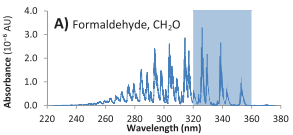
\includegraphics{Figures/HCHO/HCHOAbsorbanceDavenport.png}
      \caption{ HCHO spectrum, with a typical band of wavelengths used for DOAS path measurements.
	This is a portion of an image from \citet{Davenport2015}.}
      \label{ch_LitRev:fig:HCHOSpectrum}
    \end{figure}
    
    
    In MAX-DOAS retrievals, the measurements of light absorption are performed over several elevations in order to add some vertical resolution to the measurement of trace gas concentrations.
    An example of this is shown in figure \ref{ch_LitRev:fig:MAXDOASExample}, which was taken from \citet{Lee2015}.
    Recently MAX-DOAS has been used to examine HCHO profiles in the clean free troposphere \citep{Franco2015, Schreier2016} as well as in polluted city air \citep{Lee2015}.
    Depending on orography and atmospheric composition (ie. the influence of interfering chemicals), MAX-DOAS can be used to split the tropospheric column into two partial columns; giving a small amount of vertical resolution to HCHO measurements \citep[eg.]{Franco2015, Lee2015}.
    
    \begin{figure}
      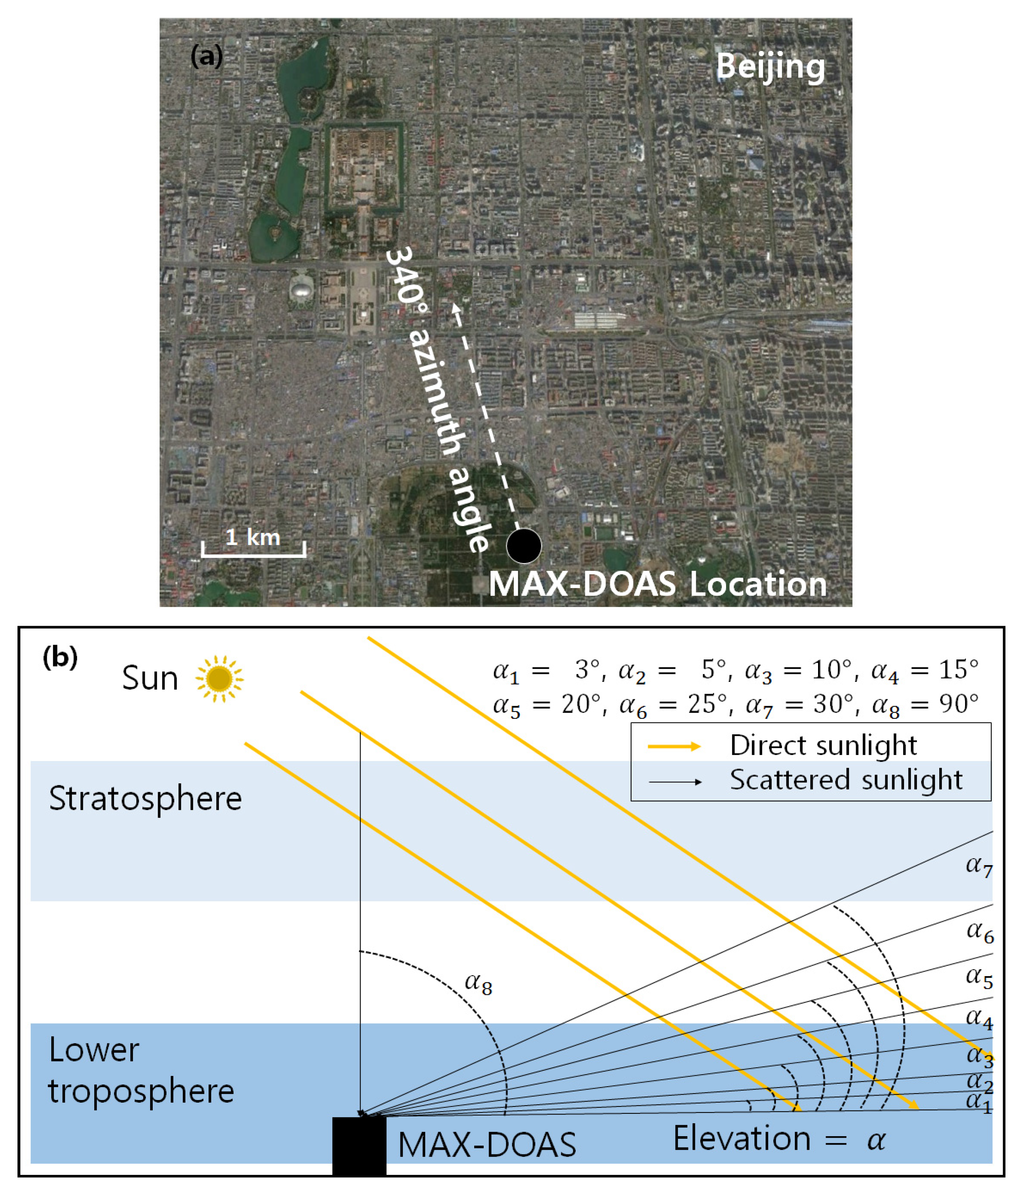
\includegraphics{Figures/MAXDoasExample.png}
      \caption{ %
        Image from \citet{Lee2015}.
      }
      \label{ch_LitRev:fig:MAXDOASExample}
    \end{figure}
    
    Other measurement techniques include chromatographic and fluorimetric methods, both of which differ widely from eachother and the spectroscopic method TODO: read \citep{Hak2005}).
    This resulted in HCHO not having a consistent network for global measurements like those for GHGs or Ozone \citep{FortemsCheiney2012}.
    
  \subsection{Relationship with glyoxyl and isoprene}
    Glyoxyl (CHOCHO) is important to us as it shares many properties with HCHO, and may provide additional information in determining isoprene emissions.
    Glyoxyl is another product of VOC oxidation in the atmosphere, with isoprene being the main source globally.
    Isoprene has been used to estimate isoprene emissions (see section \ref{ch_LitRev:sec:IsopFromHCHO}) but many uncertainties exist.
    One of these uncertainties is the yield of HCHO from isoprene, especially in low NO$_X$ environments.
    Glyoxyl could prove complementary to HCHO in constraining isoprene emissions (TODO: Read and cite Vrekoussis2009,2010, Chan Miller 2014, Alvarado 2014).
    
    Under high NO$_X$ conditions, glyoxyl forms rapidly, similarly to HCHO.
    However, glyoxyl also forms in low NO$_X$ environments both slowly (through isoprene epoxydiols), and rapidly (through di-hydroperoxide dicarbonyl compound photolysation (todo: read abstract and cite crounse(Autoxidation of Organic Compounds in the Atmosphere) 2013).
    This process is similar to the proposed mechanisms for hydroperoxyaldehydes by \citet{Peeters2014} and carbonyl nitrates (todo: read and cite M$\:{u}$ller 2014).
    
  \subsection{Satellite measurements}
    Satellite measurements of HCHO are relatively uncertain, however this can be improved by averaging over larger grid boxes or longer time scales.
    an example of this can be seen in \citet{Dufour2009}, where monthly averaging is used to decrease the measurements uncertainty.
    They examine HCHO in Europe, which is low; near the detection limit of satellite measurements.
    Taking monthly averages allows enough certainty that useful inversions can be determined to estimate the source emissions of HCHO.
    
    In satellite HCHO products, concentrations over the remote pacific ocean are sometimes used to analyse faulty instrument readings.
    This is due to the expected invariance of HCHO over this region.
    For instance GOME (an instrument which measures trace gases on board the ERS-2) corrects for an instrument artifact using modelled HCHO over the remote pacific \citep{Shim2015}.
    OMI HCHO products use a similar technique to account for sensor plate drift and changing bromine sensitivity \citep{Abad2015}
    
    For many places the tropospheric column HCHO measured by satellite is biased low, \citet{Zhu2016} examine six available datasets and show a bias of 20 - 51\% over south east USA when compared against a campaign of aircraft observations (SEAC$^4$RS).
    \citet{DeSmedt2015} also found a low bias from 20 - 40\% when comparing OMI and GOME2 observations against ground based vertical profiles, and \citet{Barkley2013} determine OMI to be 37\% low compared with aircraft measurements over Guyana.
    These bias can be corrected by improving the assumed apriori HCHO profiles which are used to calculate the AMFs of the satellite columns.
    
    The OMI measurements used in this research are recalculated using an updated estimate of HCHO profiles and validated against Wollongong total column measurements. 
    Similar to validation performed by other studies TODO: cite and exemplify a few studies ie: \citet{Zhu2016, Marais2015, Palmer2003} 
    
    Uncertainty in the OMI satellite instrument is calculated by the Smithsonian Astrophysical Observatory (SAO) group using the uncertainty in backscattered radiation retrievals \citep{Abad2015, Abad2016}.
    Another method of calculating the uncertainty is used by the Belgian Institute for Space Aeronomy (BIRA) group, who determine uncertainty from the standard deviation of HCHO over the remote pacific ocean (TODO: use both these methods for HCHO section)\citep{DeSmedt2012, DeSmedt2015}.
    
    GOME suffers from similar uncertainties to OMI, as the same general method of DOAS remote measurements are performed.
    The uncertainty from slant column fitting has been calculated for GOME to be $4\times10^{15}$ molecules cm$^{-2}$ \citep{Chance2000, Millet2006}. 
    The conversion factor for slant to vertical columns (AMF) calculation also suffers from errors; primarily from surface albedo, HCHO vertical profile apriori, aerosol, and cloud influence \citep{Millet2006}. 
    AMF uncertainties for GOME are calculated to be $1$ to $1.3\times10^{15}$ molecules cm$^{-2}$ by \citet{Shim2005}.
%----------------------------------------------------------------------------------------
%	Isoprene Section
%----------------------------------------------------------------------------------------
\section{Isoprene}
\label{ch_LitRev:sec:isoprene}

  \subsection{Basics}
    Isoprene, or 2-methylbuta-1,3-diene, is a Volatile Organic Compound (VOC) and has chemical formula of C$_5$H$_8$. 
    Isoprene effects NO$_X$ and HO$_Y$ cycling, and in the presence of NO$_X$, forms tropospheric ozone and SOAs \citep{Wagner2002, Millet2006}.
    Bottom up inventories of VOCs remain largely uncertain due to extensive extrapolation over plant functional types, changing land cover, and parameterised environmental stressors (todo: read and \citep{Guenther2000}).

  \subsection{Sources and Sinks}
    Methane and isoprene each comprise around a third of the yearly global total emission of VOCs.
    However, methane is relatively long lived (years) and is well mixed in the atmosphere while isoprene levels are very volatile and spatially diverse due to a life time of around an hour.
    Estimates put global isoprene emission at roughly 600 Tg yr$^{-1}$, emitted mostly during the day.
    Major emitters are tropical broadleafs (notably eucalypts), and scrubs \citep{Guenther2006, Arneth2008, Niinemets2010, Monks2015}.
    
    Isoprene has a short lifetime during the day, roughly an hour due to OH oxidation (todo: abstract and cite Atkinson and Arey 2003\citep{AtkinsonArey2003}).
    At night when OH concentrations have dropped, isoprene can remain in the atmosphere to be transported. 
    Typically less than half of this night time isoprene is removed through ozonolysis \citep{AtkinsonArey2003}, however, in polluted areas where high levels of NO$_X$ exist, isoprene is consumed by a different radical.
    During the night time, nitrate radicals (NO$_3$) build up, especially in areas with high NO$_X$ levels.
    In areas with high NO$_X$ levels, greater than 20\% of the isoprene emitted late in the day ends up being oxidised by the NO$_3$ radical over night \citep{Brown2009}.
    So while night time isoprene is not as highly concentrated, is does have varying biogenic and anthropogenic sinks.
    At night isoprene has affects on both NO$_X$ concentrations and ozone levels, and can form harmful SOAs \citep{Brown2009, Mao2013}.
    
    Isoprene oxidation by OH is less well understood in lower concentrations of NO.
    Initially isoprene was thought to be a sink for atmospheric oxidants \citep[eg.]{Guenther2000}.
    It was thought that in low NO environments, like those far from anthropogenic pollution and fires, oxidation of isoprene would create hydroxyhydroperoxides (ISOPOOH) and lead to low concentrations of OH and HO$_2$ (together known as HO$_X$) \citet{Paulot2009b}.
    In \citet{Paulot2009b}, the HO$_X$ levels are shown to be largely unnaffected by isoprene concentrations.
    They show that ISOPOOH is formed in yields $> 70\%$, and MACR and MVK is formed with yields $< 30\%$.
    The formation of MACR and MVK produces some HO$_X$, although not enough to close the gap.
    \citet{Paulot2009b} goes on to suggest (and provide experimental evidence) that dihydroxyperoxides (IEPOX) are formed from oxidation of the ISOPOOH, which form precursors for SOAs as well as closing the HO$_X$ concentration gap.
    They then use GEOS-Chem, modified to include IEPOX formation, to estimate that one third of isoprene peroxy radicals react with HO$_2$, and two thirds react with NO. 
    Their work showed another pathway for isoprene based SOA creation, and additionally estimated $95 \pm 45$~TgC yr$^{-1}$ IEPOX being created in the atmosphere without any inclusion in CTMs at that time.
    In \cite{Crounse2012}, MACR products are examined in various conditions and hydroxy recycling is also observed in low NO conditions. 
    
    Although understanding of OH production/recycling in these low NO conditions has been improved, many observations of OH are still quite under-predicted in models \citep{Mao2012}.
    It was shown in \citet{Mao2012}, for a remote forest in California, that the traditional method of OH measurement may be affected by instrument internally generated OH from VOC oxidation.
    This lends more credence to the current understanding of VOC oxidation as it closed the gap between measurements and model predictions.
  %\subsection{Products from isoprene}
  \subsection{Factors affecting isoprene emissions}
    
    \citet{Marais2014} examine factors affecting isoprene emissions, showing how emissions are sensitive to various environmental factors.
    Their work used MEGAN \citep{Guenther1995} and GEOS-Chem to look at how these factors affect surface ozone and particulate matter in Africa.
    One of the important uncertainties seen in MEGAN within this work is the isoprene emissions due to plant type. 
    Canopy level isoprene measurements are made using relaxed eddy accumulation (REA) at several sites in Africa.
    One plant type near a measurement site emits more than other species and it's actual distribution on a larger scale is completely unknown - leading to possible overestimations in MEGAN.
    
    \citet{Stavrakou2014} examined modelled Asian emissions and altered model parameters for temperature, plant type emission factors, incoming solar radiation (insolation) intensity, land use changes, and palm tree forest expansion.
    Changes were constrained by a network of radiation measurements and some experiments with south east Asian forest emissions - and led to reduction in isoprene emissions by a factor of two over the region.
    The Asian region is also shown to have a strong correlation with the Oceanic Niño Index (ONI), with positive anomalies associated with El Niño.
  
  \subsection{Estimates}
    It used to be thought that anthropogenic and biogenic emissions of VOCs were roughly similar (TODO abstract of \citep{Mueller1992}, and more cites).
    It's now clear that biogenic isoprene emissions are far greater than anthropogenic emissions of VOCs \citep{Guenther2006, Kefauver2014}. 
    The estimates are still fairly uncertain, as global measurements are difficult and regional emissions can be very different. 
    The lack of accuracy in BVOC emissions estimates has a large effect on determining with confidence the sources and distribution of pollutants including ozone and organic aerosols.
    Accuracy in VOC measurements is important: it has been shown that even the diurnal pattern of isoprene emissions has an effect on modelling ground level ozone \citep{Hewitt2011,Fan2004}.
    These uncertainties could explain why models of HCHO over Australia are poor at reproducing satellite measurements \citep{Stavrakou2009}.

    \citet{Guenther2006} estimates that the Australian outback is among the world's strongest isoprene emitters with forests in SE Australia having emission factors greater than 16 mg m$^{-2}$ h$^{-1}$ (see figure \ref{ch_LitRev:fig:meganisoprene}).
    These emissions factor estimates are not well verified as there is little coverage of isoprene (or other BVOC) emissions measurements over Australia.
    However, comprehensive coverage of one high yield (generally) product in the atmosphere over Australia exists in the form of satellite measurements.
    
    It is important to note that many estimates of isoprene emission are based on a few algorithms of isoprene emission which can depend greatly on input parameters \citep{Niinemets2010}.
    \citet{Yue2015} has shown that this is still a problem by looking at land carbon fluxes and modelling the sensitivity to VOC emissions estimates using two independent models of VOC emission.
    One model is photosynthesis based and estimates isoprene emissions using electron transfer energies and leaf physiology \citep{Niinemets1999}, while the other (MEGAN) uses the light and canopy temperature (\citep{Guenther1995} TODO: Arneth et al., 2007; Unger et al., 2013).
    Both are sensitive to light and temperature parameterisations.
    
    
    \begin{figure}
      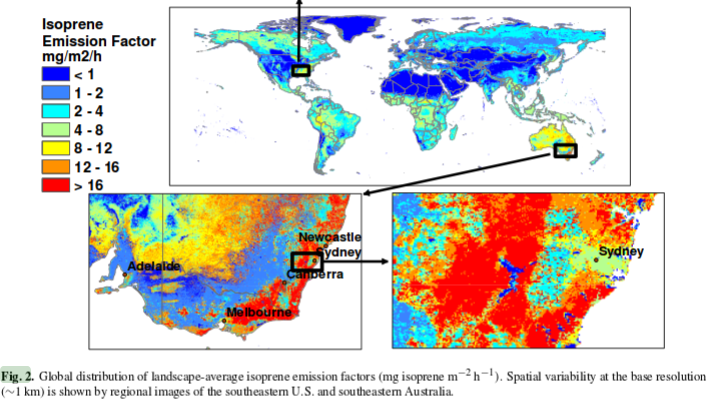
\includegraphics{Figures/MeganIsoprene1.png}
      \caption{ Part of a figure from \citet{Guenther2006} showing global isoprene emission factors. }
      \label{ch_LitRev:fig:meganisoprene}
    \end{figure}
    
  \subsection{Isoprene to HCHO}
    \label{ch_LitRev:sec:IsopFromHCHO}
    In the remote troposphere HCHO production is dominated by methane oxidation, while in the continental boundary layer (CBL) production is largely due to NMVOCs \citep{Abbot2003, Kefauver2014}.
    NMVOCs are alkanes, alkenes, aromatic hydrocarbons and isoprene.
    Isoprene is hard to measure directly due to its short lifetime and weak spectral absorption, instead formaldehyde is often used as a proxy \citep{Millet2006, Dufour2009, Marais2012, bauwens2013satellite, Kefauver2014, Bauwens2016}.
    Formaldehyde formed in the troposphere is mostly due to VOC (roughly one third each: methane, isoprene, others) oxidation.
    We can model this oxidation process in order to work out how much VOC is present based on the total HCHO.
    This requires among other things an idea of which VOCs are present and their yields of HCHO.
    
    The method used to develop top-down isoprene inference using satellites was developed initially by \citet{Palmer2001, Palmer2003}. 
    Isoprene emissions fluxes were derived using the Global Ozone Monitoring Experiment (GOME) satellite instrument.
    Palmer's method improved biogenic isoprene emissions estimates (compared with in-situ measurements) over two available inventories: the U.S. EPA Biogenic Emssions Inventory System (BEIS2) and the Global Emissions Inventory Activity (GEIA).
    This showed an inversion technique which could be used to improve large scale emissions estimates without further expensive measurement campaigns.
    
    \citet{Dufour2009} use HCHO from SCIAMACHY, and examine Europe using CHIMERE as the chemical model. 
    In their work they show that satellite measurements can reduce source emission uncertainty by a factor of two, where emissions are relatively large.
    
    
    Satellites recording reflected solar spectra use Differential Optical Absorption Spectroscopy (DOAS) to measure various trace gases in the atmosphere, including formaldehyde. 
    Formaldehyde levels in the continental boundary layer are generally dominated by chemical formation due to VOC (largely isoprene) emissions \citep{Kefauver2014}.
    
    Satellites can be used to measure the seasonal and interannual variability of HCHO over Australia.
    These records can be compared with modeled estimates of HCHO and used as a proxy to estimate isoprene emissions.
    This has been done in North America \citep{Palmer2003, Millet2006}, South America, Africa, China, Europe \citep{Dufour2009}, and recently globally \citep{FortemsCheiney2012, Bauwens2016}.
    Often these works use two forms of measurement such as satellite and aircraft data combined for validation \citep{Marais2014}.
    
    Initially studies assumed a simple linear steady-state relationship between HCHO and it's precursors \citep{Palmer2003, Palmer2006, Millet2006}.
    This allowed a simple calculation of isoprene using the measured HCHO, with estimated reaction rates and yields.
    The methodology for calculating VOCs from HCHO is laid out in \citet{Palmer2003}, and takes into account the expected lifetime and reaction rates of the precursor VOCs and HCHO.
    Assuming HCHO is produced quickly from short-lived intermediates, and the column is at steady state:
    \begin{eqnarray*}
    VOC_i \overset{k_i}{\rightarrow} Y_i HCHO
    \end{eqnarray*}
    Where $Y_i$ is HCHO yield per C atom (a measure of how much HCHO will form per gram of C from a VOC within a system), and $k_i$ is the reaction rate.
    Then assuming a steady state of atmospheric HCHO ($\Omega$ molecules $cm^{-2}$) produced by oxidation of VOCs (VOC$_i$) and no horizontal transport:
    \begin{eqnarray*}
    \Omega = \frac{1}{k_{HCHO}} \sum_{i} Y_i E_i
    \end{eqnarray*}
    Where i indexes a chemical species, $k_{HCHO}$ is the HCHO loss rate due to OH and photolysis, Y$_i$ is the molar HCHO yield from oxidation of i, and $E_i$ is emission fluxes ( C atoms $cm^{-2}s^{-1}$).
    
    Estimates of Y$_i$ can be attained from a model as shown in \citet{Millet2006}.
    This involves a reduced major axis (RMA) correllation calculation between modelled HCHO and isoprene columns, multiplied by their loss rates (to photolysis and oxidation) (as a normalising factor).  
    In high NOx environments where HCHO has a lifetime on the order of 30 minutes, it can be used to map isoprene emissions with spatial resolution from 10-100 kms.
    Horizontal transport 'smears' the HCHO signal so that source location would need to be calculated using windspeeds and loss rates \citep{Palmer2001,Palmer2003}.
    For more details on this see section \ref{ch_LitRev:sec:smearing}.
    
    Another method of correcting isoprene emissions using observed HCHO total column involves a Bayesian inversion.
    \citet{Shim2005} work with GOME HCHO observations and GEOS-Chem, looking at areas with high signal to noise ratio (higher HCHO concentrations).
    They show that the model underestimates isoprene emissions and HCHO concentrations by 14-46\%, with the corrected VOC emissions reducing the model biases to 3-25\%.
    
    The Bayesian inversion is also used in \citet{Curci2010}, where a regional CTM (CHIMERE) simulates HCHO, which is compared against OMI observed HCHO and shown to be regionally biased.
    This bias is expected to be caused by errors in MEGAN's natural isoprene emissions.
    The CHIMERE model is used to derive yields of HCHO from the various local VOCs and these are then used in estimating local emissions.
    The model is run initially with emissions of BVOCs and reactive anthropogenic VOCs (RAVOCs) turned off in order to work out the background (b) values of these compounds.
    The Bayesian inversion is used to correct regionally biased biogenic isoprene emissions by optimising these parameters in order to simulate HCHO closest to the observed HCHO levels.
    \cite{Curci2010} uses CHIMERE as the forward model to determine the relationship between HCHO (y), isorene and reactive anthropogenic VOCs (\textbf{x}), using 
    \begin{equation}
        y=\mathbf{K}x + b + \epsilon
    \end{equation}
    where $\epsilon$ are the (assumed) independent errors in measurements.
    K is the Jacobian matrix determined from CHIMERE representing the sensitivity of y to the state variable x.
    This K matrix is used in conjunction with error covariance in x to determine the Maximum A Posteriori (MAP) solution to calculate the optimal estimate of x ($\hat{x}$).
    
    TODO: Read through this list of sources on the hcho to isop process : taken from Wolfe2015
    Such techniques have informed isoprene emission inventories in North America (Abbot et al., 2003; Millet et al., 2008 \citep{Palmer2003,Millet2006,Palmer2006}), South America (\citep{Barkley2013}, 2008), Europe \citep{Curci2010,Dufour2009}, Africa \citep{Marais2012}, Asia (Fu et al., 2007; Stavrakou et al., 2014), and globally (Fortems-Cheiney et al., 2012; \citep{Shim2005}; Stavrakou et al., 2009).
    
    More recently, full inversions that better account for transport, source attribution, and chemical schemes have been implemented \citep{FortemsCheiney2012}.
    TODO: full description of this better inversion technique going through FortemsCheiney2012.
  
  \subsection{Smearing}
  \label{ch_LitRev:sec:smearing}
    The distance travelled downwind (L$_{d,i}$ by a precursor (i) before becoming HCHO can be estimated using:
    \begin{equation*}
      L_{d,i} = \frac{U}{k_i - k_{HCHO}} \ln{ \left( \frac{k_i}{k_{HCHO}} \right) }
    \end{equation*}
    where U is windspeed.
    \citet{Palmer2003} further define a smearing length scale: L$_{s,i}$ as the distance downwind where a fraction (1 - $1/e$) of the precursor is completely transformed into HCHO.
    This equation uses the initial VOC column concentration ($[VOC]_0$) at the point of emission and mass balance equations, and is as follows:
    \begin{equation}
      \frac{1}{k_{HCHO}-k_i} \left( k_{HCHO} \exp{ \left[ \frac{-k_i L_{s,i}}{U} \right]} -k_i \exp{ \left[ \frac{-k_{HCHO} L_{s,i}}{U} \right]} \right) = \frac{1}{e} 
    \end{equation}
    with limiting values L$_{s,i} \rightarrow U/k_i$ for $k_i << k_{HCHO}$, and L$_{s,i} \rightarrow U/k_{HCHO}$ for $k_{HCHO} << k_i$.  
    
    Accounting for transport of the precursors is important, especially in low NO$_X$ conditions in which isoprene has a longer lifetime (days).
    This allows horizontal transport to occur and complicates the algorithms, as can be seen by the smearing length scale which increases beyond the 100~km.
    For conditions where VOCs have a lifetime of days determining the major HCHO contributors requires a complex inversion to map HCHO columns to VOC emissions.
    
  \subsection{Measurements}
  
    There are relatively few measurements of isoprene in the southern hemisphere, including MUMBA(TODO CITE), other campaigns?, and very recently that girl from Macquarie University with an instrument in the daintree rainforest(TODO CITE, DESCRIBE?).
    Since 1997, when GOME first measured HCHO over Asia (TODO cite thomas 1998), satellites have been able to provide a total column measurement of one of the primary products of isoprene.
    
    
  \subsection{Estimates}
    There are two commonly used ways of estimating isoprene emissions, top-down or bottom-up.
    Bottom-up emission estimates generally model the flora and events which emit isoprene, like Eucalypts, factories, shrubs, leaf areas under sunlight, etc.
    Understanding how much isoprene is emitted, when and by what is more complicated than it sounds, and since little data exists with which to verify these bottom-up emission inventories they are uncertain on a large scale.
    Top-down estimates look at how much of a chemical is in the atmosphere and try to work out how much of it's major precursors were emitted.
    For isoprene this is done by looking at atmospheric HCHO enhancement, which can be largely attributed to isoprene emissions as long NO$_X$ and transport effects are accounted for.
  
  \subsection{Isoprene products}
    Isoprene forms many products with various lifetimes, here I will present an overview of some important mechanisms which affect oxidation capacity, ozone and aerosol production.
    Isoprene reacts with OH leading to peroxy radical (ISOPO$_2$) formation.
    In the presence of NO$_X$ ISOPO$_2$ forms organic nitrates after reacting with NO.
    These affect levels of both HO$_X$ (H, OH, peroxy radicals) and NO$_X$, acting as a sink (\citet{Mao2013} and references therein).
    
    The first generation of organic nitrates produced by isoprene oxidation range from 7\% to 12\%, shown in laboratory experiments (todo read abstracts and cite papers in the 3rd paragraph of intro to Mao2013),
    A portion of isoprene nitrates are recycled back to NO$_X$, so may serve as a reservoir of nitrogen and allow its transport to the boundary layer of remote regions (TODO: as prior todo).
    
    During the night isoprene is oxidised by NO$_3$ radicals, which joins to one of the double bonds and produces organic nitrates in high yield (65\% to 85\%) \citep{Mao2013}. (todo: read mao2013 para 3 cites for)
    These organic nitrates go on to produce further SOAs \citep{Rollins2009} (todo read Rollins2009).
  
    Todo: More on \citep{Mao2013} ()chemistry mechanism used in GEOS-Chem v9.02)
    For specific information on the isoprene oxidation mechanisms used by GEOS-Chem V10-01 (used in this work), see section \ref{ch_isop:sec:GEOSChemMechanisms}.
  
  \subsection{Radiative Forcing}

    
%----------------------------------------------------------------------------------------
%	SECTION 5
%----------------------------------------------------------------------------------------
\section{Dust}
\label{ch_LitRev:sec:dust}

  Australia is the greatest source of dust in the southern hemisphere producing around 120~Tg yr$^{-1}$ \citep{Li2008}, however model validation and analysis over Australia is relatively scarce with more focus applied to the northern hemisphere \citep{Fairlie2007, Ridley2013}.
  Atmospheric dust has many direct effects including reduced surface insolation, mineral transfer to remote ocean regions, and health degradation in populated areas \citep{Shao2007}.
  Direct and indirect effects of dust have many implications which are not fully understood, with many models still struggling to explain the atmospheric cycling of dust at larger scales \citep{Rotstayn2011}.

  Australian dust emissions involve various weather conditions, convolving the ENSO cycle with flooding, droughts, and winds.
  Rivers and rain build up the particulate matter in many areas, these are referred to as fluvial deposits.
  Fluvial deposits in the Eyre basin increase the dust base load, which will only have mobility during suitable dry weather conditions.
  These deposits are saltated (loosened from the surface) and transported by strong winds\citep{Zender2003}.

  Synoptic scale measurements of dust concentrations in Australia are made by the Bureau of Meteorology (BOM) and can be used to estimate dust transport caused by large storms. 
  Single storms have been estimated to move up to 2.5 Tg of dust off shore in a single day.
  Yearly dust emissions in Australia are somewhere between 10 and 110 Tg yr$^{-1}$.
  These estimates exemplify the large variability in Australian annual dust transport.

  Dust plays a large role in the oceanic carbon cycle, as dust is a major source of oceanic iron (Fe) deposition.
  Some regions in the ocean are high in nutrients, but low in chlorophyll (HNLC), due to a lack of Fe.
  Oceanic carbon cycling is a complex system in which Fe is a limiting factor, required by plankton in order to fix atmospheric nitrogen into a more bioavailable form such as ammonia.
  Atmospheric deposition into the oceans is a very poorly constrained variable in global models \citep{Grand2015}.
  Model estimates of trace element oceanic deposition are required to quantify the atmospheric impact due to a dearth of in situ measurements in remote open ocean regions.

  Measurements of dissolved iron (DFe) at very low concentrations like those found in surface ocean waters are very easily contaminated, which has contributed the the fragmentary and scarce nature of DFe ocean data sets \citep{Rijkenberg2014}.
  Recent analysis of the US Climate Variability and Predictability (CLIVAR)-CO$_{2}$ Repeat Hydrography Program predicted total deposition flux with uncertainty at a factor of 3.5 \citep{Grand2015}.
  Some headway has been made with the recent GEOTRACES program which has several transects of the major oceans and measures trace elements over multiple depths including Al, Ba, Cu, Cd, Fe, Mn, Ni, Pb, and Zn.
    
  Total iron (TFe) emissions from dust and combustion sources are estimated (by average of several global models) at approximately 35~Tg yr$^{-1}$ and 2 Tg yr$^{-1}$ respectively. A two fold increase in Fe dissolution may have occurred since 1850 due to increased anthropogenic emissions and atmospheric acidity.
  This increase may revert by 2100 due to the affects of emission regulations \citep{Myriokefalitakis2015}.
  Dust, TFe and DFe have strong temporally and spatial variability, with changes having most impact upon HnLC regions.

  Another environmental impact of dust is its contribution to fine particulate matter in the atmosphere.
  Several studies have shown that long term exposure to fine particulate matter (PM2.5) increases mortality. 
  Estimates of yearly premature deaths related to PM2.5 are $\sim$ 2-3 million \citep{Hoek2013, Krewski2009, Silva2013, Lelieveld2015}.   
  These estimates are made using global atmospheric models or model ensembles to quantify population exposure before applying epidemiological models to estimate the increased death rates.
  The main source of uncertainty in premature death rates arises from the difference and uncertainties between and within the atmospheric models.

  Dust affects global climate change through direct radiative forcing.
  Uncertainties in the atmospheric dust concentrations make accurate determination of radiative forcing from other sources more difficult \citep{IPCC_2013_chap8}.


%----------------------------------------------------------------------------------------
%	SECTION 6
%----------------------------------------------------------------------------------------
\section{Models}
\label{ch_LitRev:sec:models}

  \subsection{Chemical Transport Models}
  
    Chemical Transport Models (CTMs) simulate production, loss, and transport of chemical species.
    This is generally calculated using one or both of the Eulerian (box) or Lagrangian (puff) frames of reference.
    CTMs normally solve the continuity equations simultaneously with chemical production and loss for chemicals under inspection. 
    The continuity equations describe transport of a conserved quantity such as mass, which, solved together with production and loss of a chemical forms the basis for a CTM.
    This basis enables a record of the chemical densities and transport over time as a model runs.
    The general continuity equation links a quantity of a substance (q) to the field in which it flows and can be described by the formula:
    \begin{eqnarray*}
	\frac{\partial \rho}{\partial t} + \nabla \cdot j &=& \sigma 
    \end{eqnarray*}
    where $\rho$ is density of q in the field, t is time, $\nabla$ is divergence, j is the flux (the amount of q per unit area per unit time entering or leaving the field), and $\sigma$ is the generation of q per unit volume per unit time.
    Note that $\sigma$ can be positive or negative due to sources and sinks.

    The type of model best suited to modelling the entire earth uses the Eulerian frame of reference, where the atmosphere is broken up into 3-D boxes with densities and transport calculated and stored for arbitrary sequential steps in time at each location.
    The mass balance equation must be satisfied in any realistic long term box model and is as follows: 
    \begin{align*}
	\frac{dm}{dt} &=& \sum{sources}-\sum{sinks} \\
	&=& F_{in} + E + P - F_{out} - L - D 
    \end{align*}
    where m is mass of a chemical, E and D are emission and deposition, P and L are production and loss, and F is chemical transport in and out, as shown in figure \ref{ch_LitRev:fig:boxmodel}.
    Many chemical species interact with each other through production and loss. 
    Any large chemical model will solve this mass balance equation over highly coupled arrays of partial differential equations which can be complex and time consuming.

    In many CTMs the isoprene emissions are calculated elsewhere with their own models (EG: \citet{Guenther2006}).
    These estimates can then be used as boundary conditions.
    Trace gases with short lifetimes and complex chemistry such as isoprene are often hard to measure which makes verifying model estimates difficult.

    \begin{figure}
      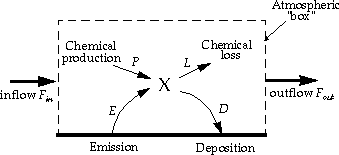
\includegraphics{Figures/boxmodel.png}
      \caption{ Standard box model parameters, image taken from \citet{Jacob_1999_book}. }
      \label{ch_LitRev:fig:boxmodel}
    \end{figure}

  \subsection{GEOS-Chem}
  
    GEOS-Chem is a well supported global, Eulerian CTM with a state of the science chemical mechanism, with transport driven by meteorological input from the Goddard Earth Observing System (GEOS) of the NASA Global Modeling and Assimilation Office (GMAO).
    GEOS-Chem simulates more than 100 chemical species from the earth's surface up to the edge of space (0.01 hPa) and can be used in combination with remote and in-situ sensing data to give a verifiable estimate of atmospheric gases and aerosols.
    It was developed, and is maintained, by Harvard University staff as well as users and researchers worldwide. 
    Several driving meteorological fields exist with different resolutions, the finest at 0.25 by 0.3125$^\circ$ horizontally at 5 minute time steps with 72 vertical levels.
    
   GEOS-Chem has boundary conditions based on several meteorological and emissions inventories, the following are the versions of theses used by GEOS-Chem v 10.01. 
   Meteorological fields can be driven by NASA's GEOS-5 data (0.5$^{\circ}$ x 0.666$^{\circ}$) (TODO:Chen et al., 2009), which exists up to 2013, or GEOS-FP data (0.25$^{\circ}$ x 0.3125$^{\circ}$).
   Fire emissions come from the GFED4 product \citep{Giglio2013}. Anthropogenic VOC emissions come from the EDGAR inventory, while biogenic VOC emissions are coupled to the MEGAN model TODO:cites.

    Combining satellite data with model outcomes provides a platform for the understanding of natural processes to be tested now and into the future over Australia and anywhere with few in-situ measurements.
    Due to the low availability of in-situ data covering most of the Australian continent, a combination of the models with satellite data may provide improved understanding of emissions from Australian landscapes.
    Improved emissions estimates will in turn improve the accuracy of CTMs, providing better predictions of atmospheric composition and its response to ongoing environmental change.

%----------------------------------------------------------------------------------------
%	SECTION 7
%----------------------------------------------------------------------------------------
\section{Satellites}
\label{ch_LitRev:sec:satellites}

  \subsection{Useful satellites}
    Several satellites provide long term trace gas observations with near complete global coverage, including the ERS-2 launched in April 1995 which houses the GOME ultraviolet and visible (UV-Vis) spectrometer, the AURA launched in July 2004 which houses the OMI UV-Vis spectrometer, the MetOp-A and B launched in October 2006 and September 2012 respectively both housing a GOME-2 UV-Vis spectrometer.
    These satellites are on Low Earth Orbit (LEO) trajectories and overpass any area up to once per day. 
    They record near nadir (nearly vertical) reflected spectra between around 250-700~nm split into spectral components at around $0.3$~nm in order to calculate trace gases including O$_3$, NO$_2$, and HCHO.
    An example of a spectrum retrieved from the GOME-2 instrument is given in figure \ref{ch_LitRev:fig:gomeproducts}.

    \begin{figure}
      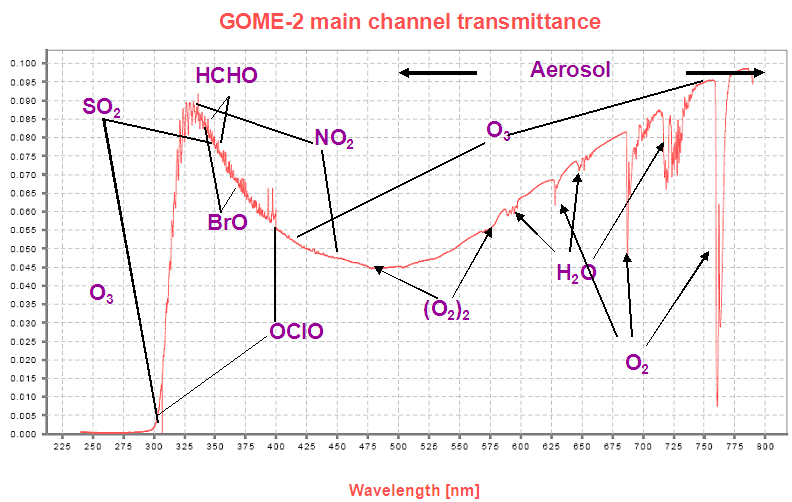
\includegraphics[width=\textwidth]{Figures/GOME_SPECTRUM.jpg}
      \caption{An example spectrum showing interferences used for species concentration measurements by GOME-2. Image by EUMETSAT and ESA \citep{GOME2Image}.}
      \label{ch_LitRev:fig:gomeproducts}
    \end{figure}

    
    Formaldehyde (HCHO) is often used as a proxy to estimate isoprene emissions \citep{Marais2012,bauwens2013satellite}.
    Satellites can use DOAS techniques with radiative transfer calculations on solar radiation absorption spectra to measure column HCHO (eg: \citet{Leue2001}).
    Several public data servers are available which include products from the satellites just mentioned, including NASA's Mirador (http://mirador.gsfc.nasa.gov/) and the Belgian Institute for Space Aeronomy (IASB-BIRA) Aeronomie site (http://h2co.aeronomie.be/).

    Instruments including MODIS on board the AQUA and TERRA satellites are able to determine aerosol optical depth (AOD), a measure of atmospheric scatter and absorbance. 
    An AOD of under 0.05 indicates a clear sky, while values of 1 or greater indicate increasingly hazy conditions.
    This is an important atmospheric property allowing us to track dust storms and pollution events as well as determine where measurements from other instruments may be compromised by high interference.
    Satellite measured AOD requires validation by more accurate ground based instruments like those of AERONET which uses more than 200 sun photometers scattered globally. 
  
  \subsection{Comparisons with Models}
  
    DOAS methods can be heavily influenced by the initial estimates of a trace gas profile (the apriori) which is often produced by modelling, so when comparing models of these trace gases to satellite measurements extra care needs to be taken to avoid introducing bias from unrealistic a priori assumptions.
    One way to remove these apriori influences is through the satellite's averaging kernal, which takes into account the vertical profile of the modelled trace gas and instrument sensitivity to the trace gas \citep{Eskes2003, Palmer2001}.
    Measurements done using DOAS often apply a forward radiative transfer model (RTM) such as LIDORT in order to determine a trace gas's radiative properties at various altitudes.
  
  \subsection{DOAS}
    TODO: some of this is repeated in isoprene chapter satellite section.
    
    The DOAS technique uses solar radiation absorption spectra to measure trace gases through paths of light.
    The RTM used in DOAS techniques is based on Beer's law relating the attenuation of light to the properties of the medium it travels through.
    Beer's law states that $ T = I/I_0 = e^{-\tau} $ with T being transmittance, $\tau$ being optical depth, and I, I$_0$ being radiant flux received at instrument and emitted at source respectively.
    Using 
    $ \tau_i = \int \rho_i \beta_i ds $ gives us:
    $$ I = I_0 \exp {\left( \Sigma_i \int \rho_i \beta_i ds \right) } $$
    Where i represents a chemical species index, $\rho$ is a species density(molecules per cm$^3$), $\beta$ is the scattering and absorption cross section area (cm$^2$), and the integral over ds represents integration over the path from light source to instrument.
    The forward RTM used for satellite data products also involves functions representing extinction from Mie and Rayleigh scattering, and the efficiency of these on intensities from the trace gas under inspection, as well as accounting for various atmospheric parameters which may or may not be estimated (e.g. albedo).
    
    To convert the trace gas profile from a reflected solar radiance column (slanted along the light path) into a purely vertical column requires calculations of an air mass factor (AMF).
    In satellite data, the AMF is typically a scalar value for each horizontal grid point which will equal the ratio of the total vertical column density to the total slant column density. This value should also account for instrument sensitivities to various wavelengths at various altitudes, and is unique for each trace gas under consideration.
  
 % Literature Review

% Chapter 2 (probably)
% STTs

\chapter{Stratosphere to Troposphere Transport of ozone} % Main chapter title
\label{ch_o3}

%----------------------------------------------------------------------------------------
%	Ozone Section
% 	TODO:SOME PORTION OF THIS SHOULD BE IN INTRO, to be worked out much later
%----------------------------------------------------------------------------------------
\section{Background}
  \label{ch_o3:sec:ozone}

  \subsection{Historical estimates}
    Tropospheric ozone is important for both air quality and climate change. 
    The impact of stratospheric ozone on the troposphere is dependent on weather, season, temperature, and many other factors. 
    For example changing ozone in the tropical tropopause layer by 5\% causes 0.5 K dec$^{-1}$ radiative heating \citep{Forster2007}.
    In Australia, records of ozone profiles provided by the Department of the Environment can be used to determine how often stratospheric ozone descends into the troposphere.

    Over the industrial period, tropospheric ozone, which is the third most potent greenhouse gas, has been estimated to exert a radiative forcing equivalent to a quarter of the CO2 forcing. 
    Ozone is present in the troposphere due to a variety of dynamical and photochemical processes, including downward  transport from the ozone-rich stratosphere and anthropogenic pollution.
    The primary sources of tropospheric ozone are chemical creation and stratospheric input, estimated using a model ensemble to be $5100\pm600$ Tg/yr and $550\pm170$ Tg/yr, respectively \citep{Stevenson2006}.
    The primary sinks are chemical destruction and dry deposition, estimated to be $4700\pm700$ Tg/yr and $1000\pm200$ Tg/yr, respectively \citep{Stevenson2006}.
    
    
    ``Further sources of uncertainty in the ozone RF stem from uncertainties in precursor emissions (natural and anthro-pogenic), as well as changes in climate and stratospheric ozone'' \citep{Stevenson2013}.

  \subsection{Tropospheric production}
  
    Ozone is a toxic trace gas which increases mortality rates when populations are exposed for extended periods of time.
    The amount of global premature deaths per year due to atmospheric ozone exposure has recently been estimated at $\sim$150-470 thousand \citep{Silva_2013, Lelieveld_2015}.
    Long term effects of ozone overexposure increase the risk of respiratory disease and may also increase other cardiopulmonary risks \citep{Jerrett_2009}.
    Further tropospheric ozone enhancements are projected to drive reductions in global crop yields equivalent to losses of up to \$USD$_{2000}$ 35 billion per year by 2030 \citep{Avnery2011}, along with detrimental health outcomes equivalent to $\sim$\$USD$_{2000}$11.8 billion per year by 2050 \citep{Selin2009}.

    The Ambient Air Quality (AAQ) National Environment Protection Measure (NEPM), which is the Australian framework for air quality measurement and reporting aiming for ``adequate protection of human health and well-being'' has set national standards and benchmarks for reporting. The NEPM covers six chemical groups including Ozone (O$_3$), and the benchmarks are shown in figure \ref{ch1:fig:nepm}.

    \begin{figure}[!htbp]
      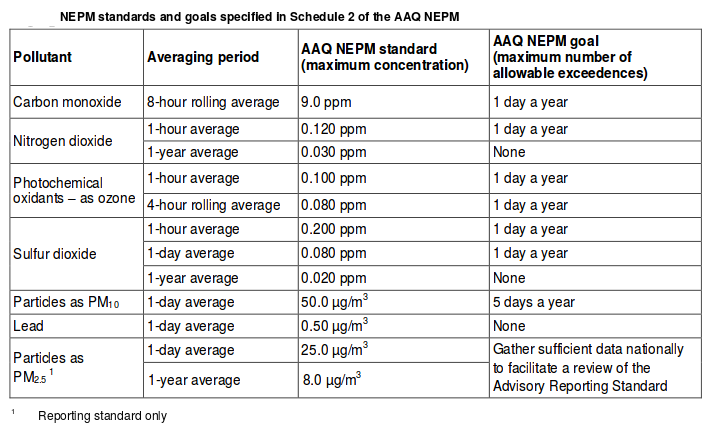
\includegraphics[width=\textwidth]{Figures/NEPMStandards.png}
      \caption{ NEPM standards taken from National Environment Protection Council annual report 2012-2013 \citep{nepc_annuals}. }
      \label{ch1:fig:nepm}
    \end{figure}
    
    The primary source of ozone in the lower troposphere is chemical formation following emissions of precursor gases, including VOCs, and NO$_X$.
    Globally the greatest sources of NO$_X$ include fossil fuel combustion ($\sim$50\%), biomass burning ($\sim$20\%), lightning, and microbial activity in soils \citep{Delmas_1997}.
    Estimates using CHASER (a global Chemical Transport Model (CTM)) constrained by measurements from two satellites as well as the in-situ measurements taken through LIDAR and aircraft (INTEX-B) put global tropospheric NO$_X$ emissions at 45.4 TgN yr$^{-1}$ in 2005 \citep{Miyazaki2011}.

    The majority of this chemical formation is due to photochemical oxidation of carbon monoxide (CO), methane (CH$_4$), and other Volatile Organic Chemicals (VOCs) in the presence of nitrogen oxides (NO$_X$ $\equiv$ NO $+$ NO$_2$) \citep{Stevenson2006}.

    Photolysis of NO$_2$ forms NO + O(3P), which combines with O$_2$ to form O$_3$, leading to reaction with NO to form NO$_2$ + O$_2$.
    These reactions reach a steady state where O$_3$ is proportional to the ratio between NO$_2$ and NO \citep{Sillman2002}.
    The following formulae show an example of this with CO, however, similar reactions occur for many VOCs:
    \begin{align}
      NO_2 + hv &\overset{k_1}{\rightarrow}& NO + O({}^3 P) \\
      O({}^3 P) + O_2 &\overset{M}{\rightarrow}& O_3 \\
      NO + O_3 &\overset{k_2}{\rightarrow}& NO_2 + O_2 \\
      \left[O_3\right] &\sim& \frac{k_1}{k_2} \frac{\left[NO_2\right]}{\left[NO\right]} \\
      OH + CO &{\rightarrow}& HOCO \\
      HOCO + O_2 &{\rightarrow}& HO_2 + CO_2 \\
      HO_2 + NO &{\rightarrow}& OH + NO_2 \\
    \end{align}
    where $k_1$ and $k_2$ are reaction rates, and hv represents photons.
    The balance of these reactions is:
    \begin{equation} CO + 2O_2 + hv {\rightarrow} CO_2 + O_3 \end{equation}
    Note that this reaction pathway only occurs during the day.

    Isoprene (C$_5$H$_8$) is a precursor to ozone through radical oxidative chemistry. Isoprene in the atmosphere reacts rapidly with hydroxyl radicals (OH) and then O$_2$ to form peroxy radicals (RO$_2$).
    These react with nitrogen oxides and can lead to ground-level ozone formation similarly to the CO reaction listed prior.

    Formaldehyde (HCHO) together with NO$_2$ regulate tropospheric oxidation capacity through O$_3$ production, as well as being health hazards.
    The HCHO/NO$_2$ ratio can be used to determine whether surface O$_3$ is NO$_2$ or VOC limited \citep{Mahajan2015}.
    If O$_3$ is NO$_2$ limited then an increase in NO$_2$ will increase O$_3$ levels while an increase in HCHO will not, and vice versa when O$_3$ is HCHO limited.
    NO$_2$ is a common pollutant in populated areas, released primarily by combustion in power generation and transport. 
    Outside of cities in Australia, VOCs and NOx are emitted from biogenic sources, although lightning, and biomass burning (most clearly in the Northern Territory) also play a role \citep{Guenther2006, VanDerA2008}.

  \subsection{Stratosphere to Troposphere ozone Transport (STT)}
  
    While the amount of tropospheric ozone is small compared with that found in the stratosphere, it is an important constituent.
    Ozone-rich air mixes irreversibly down from the stratosphere during meteorologically conducive conditions \citep{Sprenger2003,Mihalikova2012}; these are referred to as Statosphere - Troposphere Transport events (STTs). 
    In the extra-tropics, STTs most commonly occur during synoptic-scale tropopause folds \citep{Sprenger2003} and are characterised by tongues of high Potential Vorticity (PV) air descending to low altitudes. 
    PV is a metric which can be used to determine whether a parcel of air is stratospheric, based on its local rotation and stratification.
    Within the troposphere PV values are typically low, increasing rapidly into the stratosphere due to the increased static stability.
    
    These ozone rich tongues become elongated and filaments separate from the tongue which mix into tropospheric air.
    Stratospheric ozone brought deeper (lower) into the troposphere is more likely to affect the surface ozone budget and tropospheric chemistry \citep{Zanis2003,Langford_2009}.
    A high correlation is found between lower stratospheric and tropospheric ozone \citep{Terao2008} with the highest STT associated with the jet-streams over the oceans in winter.
    Irreversible STT of ozone is important for explaining tropospheric ozone variability \citep{Tang2010}.
    Stratosphere to Troposphere ozone transport can potentially increase regional surface ozone levels above safe levels \citep{Zhang2014}.
    
    While photochemical production is the dominant source, stratosphere to troposphere transport of ozone is also important and climate change may drastically increase this quantity \citep{Hegglin_2009}.
    In a future climate, a warmer, wetter troposphere will change the chemical processing of ozone.
    Dynamical processes such as STT, boundary layer ventilation and convection changes will alter tropospheric ozone distributions.
    \citet{Hegglin_2009} estimate that climate change will lead to increased STT of the order of 30 (121) Tg yr$^{-1}$ relative to 1965 in the southern (northern) hemisphere due to an acceleration in the Brewer Dobson circulation. 
    
    STT events are characterised in the ozonesondes' vertical profiles of ozone as altitudes in the troposphere where the ozone mixing ratio exceeds a specified threshold. 
    Usually stratospheric ozone mixes irreversibly down into the troposphere in a synoptic-scale tongue of air: the vertical ozone profile observed by the ozonesonde depends upon the time in this cycle that it is observed \citep{Sprenger2003}. 
    As such, the altitude of the tropospheric ozone peak due to an STT event, and the amplitude of the event above the background tropospheric ozone profile, vary in space and time.

%----------------------------------------------------------------------------------------
%	Ozone Sondes
%----------------------------------------------------------------------------------------

\section{Instruments and data sets}
  \subsection{Atmospheric Infrared Sounder (AIRS)}
    AIRS is an instrument on board NASA's AQUA satellite, which overpasses the globe roughly daily on a sun-synchronous orbit gathering measurments at 1:30pm local time.
    AIRS is a high spectral resolution spectrometer with 2378 bands in the thermal infrared (3.7 - 15.4 $\mu$m) and 4 bands in the visible (0.4 - 1.0 $\mu$m).
    One of the products shared by NASA is total column carbon monoxide (AIRS3STD \citep{AIRS3STD}).
    Using this product to exclude possible fire plume transport from STT analysis is done in section \ref{ch_o3:sec:airs_fire_filter}.
  
  \subsection{Sondes}
  
    Ozonesondes are weather balloons with an attached instrument which measures ozone concentrations roughly every 100m up to around 30km. These ozonesondes provide a high-vertical resolution profile of ozone.
    
    In this work sonde data from three sites are utilised: Davis (lat, lon, UTC~$+7$), Macquarie Island (lat, lon, UTC~$+11$), and Melbourne (lat, lon, UTC~$+11$).
    Ozonesondes are launched approximately weekly from these three sites, we exame data from up to 2013, starting in 2004 at Melbourne and Macquarie Island, and 2006 at Davis.
    More frequent ozonesonde launches occur at Davis during the spring ozone hole season than at other times of the year \citep{Alexander2013}.
  
  \subsection{European Centre for Medium-Range Weather Forecasts (ECMWF) Re-Analysis - Interim data set (ERA-I)}
    Ozonesondes provide much higher vertical resolution profiles of ozone than that available from reanalyses products.
    The downside is that one data point per week from an ozonesonde release is too low to be in itself useful to diagnose the evolution of STT exchange over time-scales associated with normal synoptic scale weather patterns present in the extra-tropics.
    The ECMWF provides a useful meteorological model based on assimilated data.
    Here, ozonesonde data are supplemented with the ERA-I dataset \citep{Dee2011} to enable construction of an STT exchange climatology.
    The dataset is called a re-analysis due to the fact that the whole timeline gets re-run when the climatological model is updated.
    This provides uniform data output over a long time period.
    
    The ERA-I data we used for synoptic weather was of one degree horizontal resolution with pressure levels at 200, 300, 400, and 500 hPa.
    For individual cases ERA-I data was downloaded at .25 degree horizontal resolution with the full 34 pressure levels from 1000 to 1 hPa.
    Note that 34 levels up to the top of the atmosphere is not enough to determine vertical transport when considering only a single vertical profile, however a precise view of coincident weather can determine probable cause of ozone flux.
    

%----------------------------------------------------------------------------------------
%	STT Detection Method
%----------------------------------------------------------------------------------------
\section{STT Detection}

  \subsection{Aim}
    Using several years of ozonesonde flights from three locations spanning the latitudes of the Southern Ocean, we create and examine a quantitative method for detecting ozone STT events from ozone vertical profiles.
    With a quantitative method of STT detection characterisation of the seasonal cycle of STT events and determination of their contribution to the total amount of tropospheric ozone is possible.
    Examination of the ozone intrusions and case studies allows us to relate these STT to meteorological events.
    Finally we use the same filtered sonde data in order to extract a lower bound estimate of how much of the tropospheric column ozone is due to STT events.

  \subsection{Tropopause Heights}
    Two definitions of the tropopause height are calculated: the standard lapse rate tropopause \citep{WMO1957}, and the ozone tropopause \citep{Bethan1996}.
    At Davis, the ozone tropopause defintion is modified for polar sites, following \citet{Tomikawa2009,Alexander2013}. 
    While the ozone tropopause can be less robust during stratosphere-troposphere exchange, it performs better than the lapse rate tropopause at polar latitudes in winter and near jet streams in the lower stratosphere \citep{Bethan1996}. The lower of these two tropopause altitude-definitions is referred to as the tropopause for this study.
    This choice of the lowest altitude of the tropopause avoids occasional unrealistically high tropopause heights due to perturbed ozone or temperature measurements.

    The monthly mean tropopause altitudes at each location are shown in Figure~\ref{ch_o3:fig:seasonaltpheights}, along with the subset of altitudes from profiles for which an STT event was determined. 
    The seasonal cycle in tropopause altitude at Melbourne is clearly apparent, as is the decreasing tropopause altitude poleward. 
    Seasonally averaged ozone as recorded over the three stations (Figure \ref{ch_o3:fig:seasonaltropozone}) shows increased ozone extending down through the stratosphere during the peak STT months over Melbourne.
    It is worth noting that tropopause altitudes at Davis may exceed 11~km altitude under certain synoptic conditions \citep{Alexander2013}: the relation of tropopause altitude with individual STT events will be investigated in detail below.

    \begin{figure}\begin{center}
      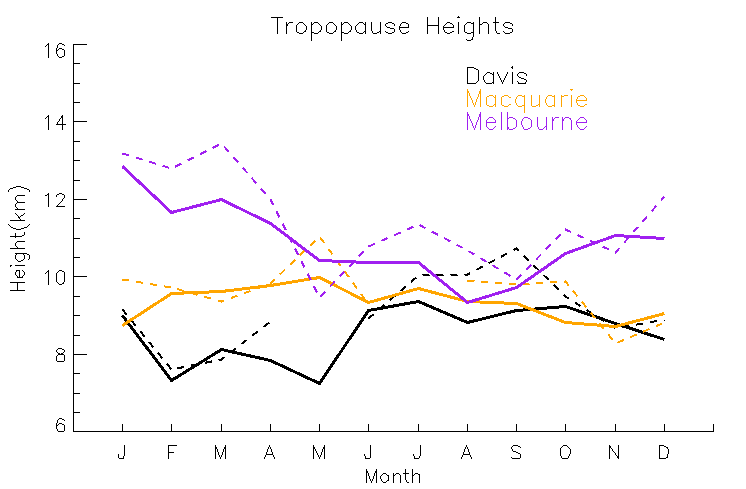
\includegraphics[width=0.8\columnwidth]{Figures/Ozone/tpheights.png}
      \caption{
	Monthly mean tropopause altitudes (minimum of lapse-rate and ozone defined tropopauses). Dashed lines show 'event only' seasonal tropopause altitudes.%
      }
      \label{ch_o3:fig:seasonaltpheights}
    \end{center}\end{figure}

    \begin{figure}\begin{center}
      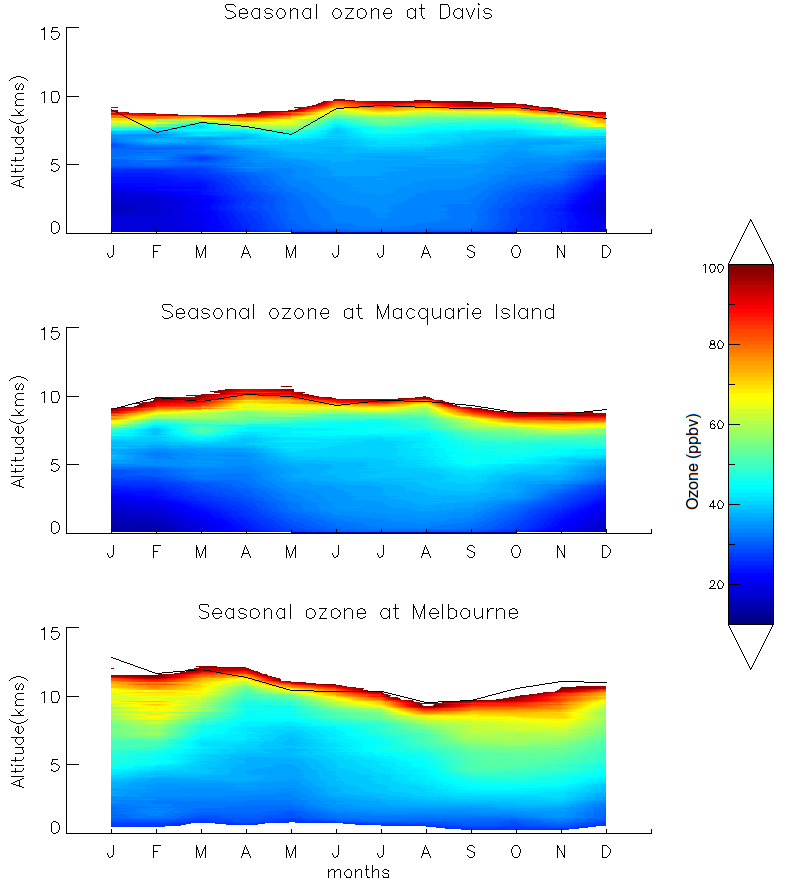
\includegraphics[width=0.8\columnwidth]{Figures/Ozone/seasonaltropozone.png}
      \caption{
	Seasonally averaged ozone over Davis, Macquarie, and Melbourne measured by ozonesondes.
	Black solid lines show seasonal tropopause heights.%
      }
      \label{ch_o3:fig:seasonaltropozone}
    \end{center}\end{figure}
    
  \subsection{Fourier bandwidth (or bandpass) Filtering}
    \label{ch_o3:sec:bandpassfilter}
    A Fourier bandwidth filter can remove components of a line based on the components frequency. 
    For example: a noisy ozone profile can be ’cleaned’ by removing the high frequency components, while growth of ozone with altitude in the profile can be removed as a low frequency component. 
    
    TODO: Add description, equation(s) and maybe a simple example plot here as well as limits of filter.
    The basic idea of a Fourier bandwidth filter is that any finite length function can be written as a series of trigonometric functions:
    \begin{equation} \label{ch_o3:eqn:FourierSeries}
      f(t) = \Sigma_i C_{w_i} \cos \left( w_i t - \theta_i \right)
    \end{equation}
    
    Once we split our function into specific frequencies ($w_i$) we can simply remove the terms which fall outside our desired wavelength range.
    One limitation is that the reconstructed function may be quite different at either end of the input range.
    
    In the continuous spatial domain, this is done is through taking the Fourier transform which can convert our function to a complex frequency domain:
    \begin{equation*}
      F(w) = \frac{1}{\sqrt{2\pi}}\int_{-\infty}^{\infty}{ f(t) e^{-iwt} \mathrm{d}t }
    \end{equation*}
    where t describes the spatial input range (in our case altitude).
    Then it's possible to remove the portion of the function outside the desired frequency before inverting the Fourier transform:
    \begin{equation*}
      f(t) = \frac{1}{\sqrt{2\pi}}\int_{-\infty}^{\infty}{ F(w) e^{iwt} \mathrm{d}w }
    \end{equation*}
    
    This whole process is slightly changed when we consider discrete dimensions as we must whenever solving numerically or handling real world resolved datasets.
    There is a ``shortcut'' method which 
    
    
  \subsection{Bandwidth filter applied to ozonesondes}
    
    With a Fourier bandwidth filter used on ozone profiles over Davis, Macquarie, and Melbourne we quantitatively determine instances of Stratosphere to Troposphere Transport events through the following method.
    The vertical profiles of ozone volume mixing ratio are linearly interpolated to a regular grid with 20m resolution up to 14km altitude and are then bandpass filtered so as to retain perturbations which have vertical scales between 0.5km - 5km. 
    The choice of band limits is set empirically, but we note that to define an STT event, a clear increase above the background ozone level is needed, and a vertical limit of $\sim 5$~km removes seasonal-scale effects. 
    The ozone perturbation profile is analysed at altitudes from 4~km above the surface (to avoid surface pollution events) and 1~km below the tropopause (to avoid the sharp transition to stratospheric air producing spurious false positives). 
    Perturbations above the 99~th percentile (locally) of all ozone levels are initially classified as STT events.
    
    In order to remove unclear 'near tropopause' anomalies we remove events where the gradient between the maximum ozone peak and the ozone at 1~km below the tropopause is greater than $-20$~ppbv~km$^{-1}$ and simultaneously require that the perturbation profile does not drop below zero between the event peak and the tropopause.
    The addition of these filters removes several events, each with an ozone peak which could not be definitively said to be seperated from the stratosphere.
    
    To provide a conservative estimate of ozone flux into the troposphere for each event, the ozone concentration is integrated vertically over the interval for which an STT event is identified.
    An example of an ozone profile is illustrated in Figure~\ref{ch_o3:fig:filterEG} and indicates how the algorithm detects an STT event, defines the event boundaries, and calculates the ozone flux.
    
    \begin{figure}[!htbp]
      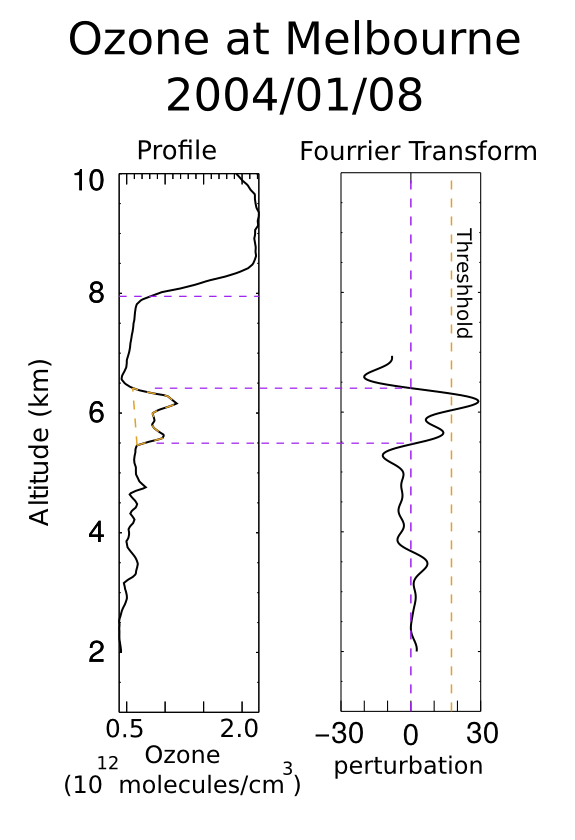
\includegraphics[width=\columnwidth]{Figures/Ozone/filtereg.png}
      \caption{ (a) An ozone profile between 2km altitude and the tropopause (indicated by the dashed vertical line).
      The 'flux' area shows the estimate of stratospheric impact on tropospheric ozone.
      (b) The 99th percentile of filtered ozone perturbations (green dashed line) and the technique for determining the vertical extent of the 'event' (red dashed and solid lines).%
      }
      \label{ch_o3:fig:filterEG}
    \end{figure}
    
  \subsection{Case Studies}
    We examine two STT case studies in detail to illustrate the synoptic scale conditions in which they can occur above Melbourne.

    A cut-off low pressure system passed over Melbourne on 3~February 2005 (Figure~\ref{ch_o3:fig:MelbourneCases}b).
    The ozonesonde profile indicated low lapse-rate and ozonesonde tropopauses (both $> 450$~hPa, see Figure~\ref{ch_o3:fig:MelbourneCases}a). 
    An ozone intrusion into the troposphere is identified by our detection algorithm at $\sim520$~hPa.

    STT events also occur during frontal passages, an example of which is illustrated in Figure~\ref{ch_o3:fig:MelbourneCases}d over south-eastern Australia.
    The tropopauses are much higher at this time and an ozone intrusion is identified centred around 200~hPa.
    Note the separation between this intrusion and the ozone tropopause (marked by the green dashed line), indicating the start of the stratosphere above Melbourne.
    During the frontal passage, stratospheric air descends and streamers of ozone-rich air likely break off and mix into the troposphere \citep{Sprenger2003}.
    TODO: talk about pvu lines here.

    The relative humidity profiles are anticorrelated with ozone in the upper troposphere for these events, indicating again the stratospheric origin of the ozone-rich air mass.
    TODO: show latlon plots for the sites and describe lowered tropopause in more detail here.
    Some of this stratospheric air gets mixed into the troposphere, with one ozonesonde column showing an intrusion at around 200 hPa, with dry ozone rich air peaking below the tropopause(Figure \ref{ch_o3:fig:MelbourneCases}c).
    
    \begin{figure}[!htbp]
      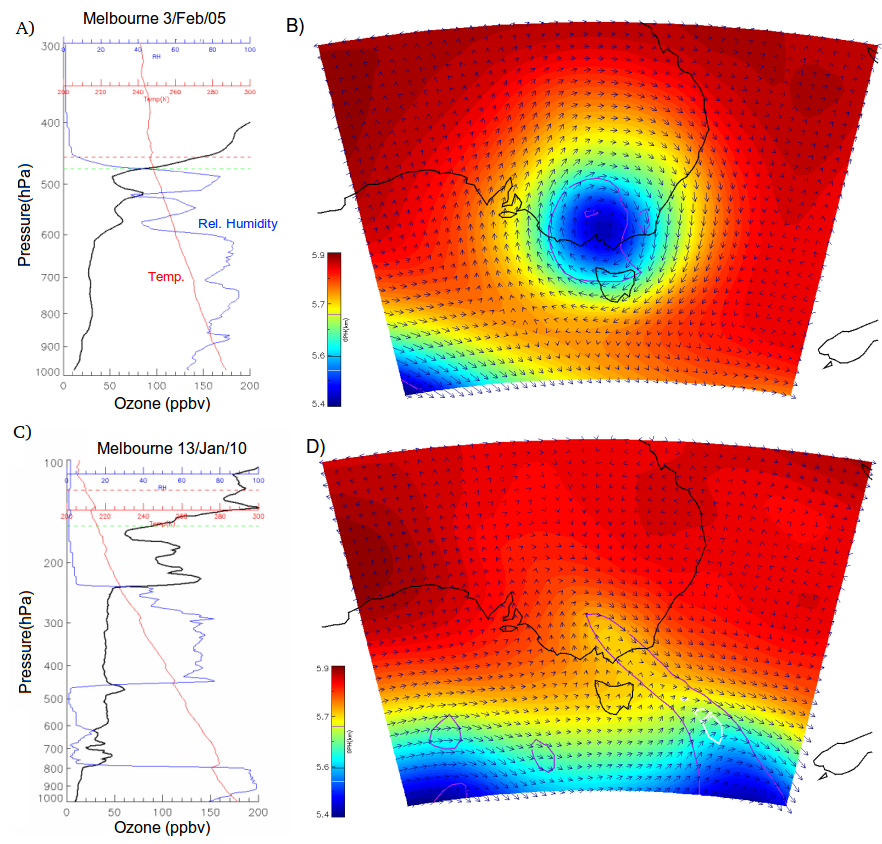
\includegraphics[width=\columnwidth]{Figures/Ozone/Cases}
      \caption{
	Vertical profiles show ozone ppbv (black line), relative humidity (blue line), and temperature (red line) for (a) 3~February 2005 and (c) 13~January 2010. Synoptic weather maps show the 500 hPa pressure level taken from the ERA-Interim reanalysis on (b) 3~February 2005 and (d) 13~January 2010. 
	Vectors show wind direction and speed while the colour indicates the geopotential height. 
	Also visible are the line contours of potential vorticity units, 1 PVU in purple and 2 PVU (often used to determine dynamical tropopause height) in white.}
      \label{ch_o3:fig:MelbourneCases}
    \end{figure}
    
  \subsection{Site summaries}
    Running the ozonesonde dataset through our bandpass filter and analysing the results allows an overview of the yearly cycle and event characteristics.
    These seasonal cycles and event characteristics for each of the three locations are presented in Figure~\ref{ch_o3:fig:SummaryMelbourne} to Figure~\ref{ch_o3:fig:SummaryDavis}.
    There is an annual cycle in the occurrence frequency of STT events (with a summertime peak) above Melbourne and Macquarie Island. However, the occurrence frequency of STT events above Davis is relatively constant throughout the year.

    The majority of events occur within 3~km of the tropopause at both Melbourne and Macquarie Island, and within 2~km of the tropopause at Davis. 
    STT event altitudes most commonly occur at 6 -- 10~km above Melbourne and below 8~km at Davis but are distributed more evenly in altitude at Macquarie Island. 
    
    \begin{figure}[!htbp]
      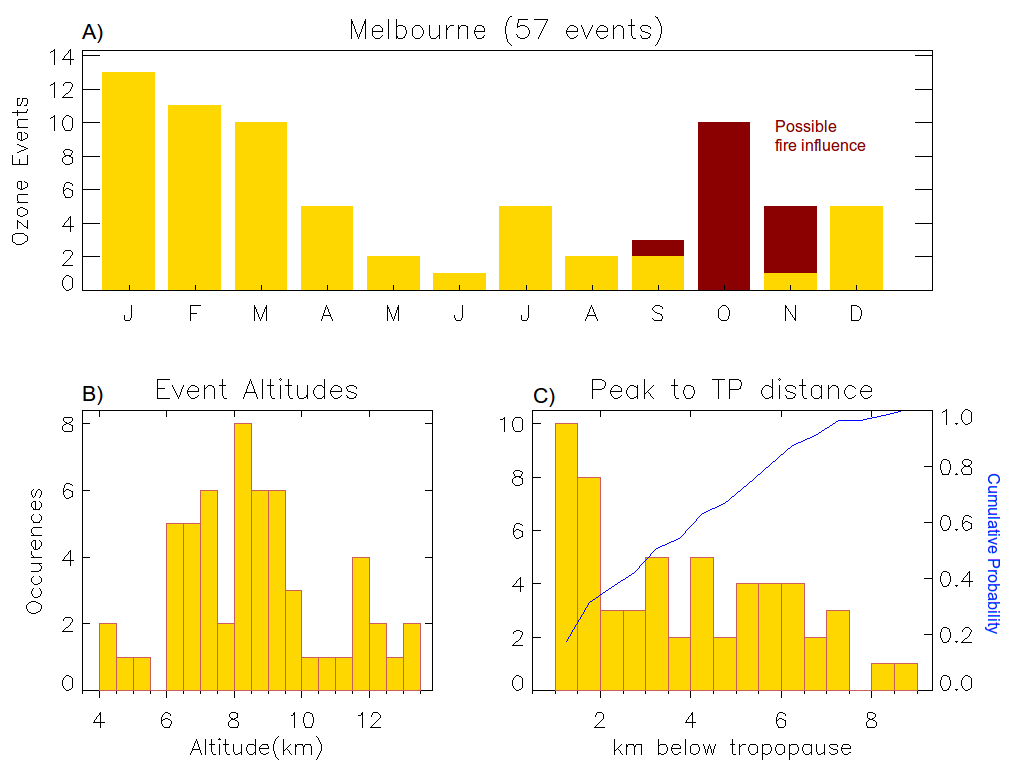
\includegraphics[width=0.8\columnwidth]{Figures/Ozone/Summary_Melb}
      \caption{
	The climatology of STT events at Melbourne: (A) Events sorted by month from the entire Melbourne ozonesonde dataset. The events filtered out as possibly smoke plume influenced are indicated in red. (B) The occurrence distribution of the ozone peak altitude. (C) The distance between the ozone peak and the tropopause (bars)  and the cumulative probability function of these distances (blue line).%
      }
      \label{ch_o3:fig:SummaryMelbourne}
    \end{figure}

    \begin{figure}[!htbp]
      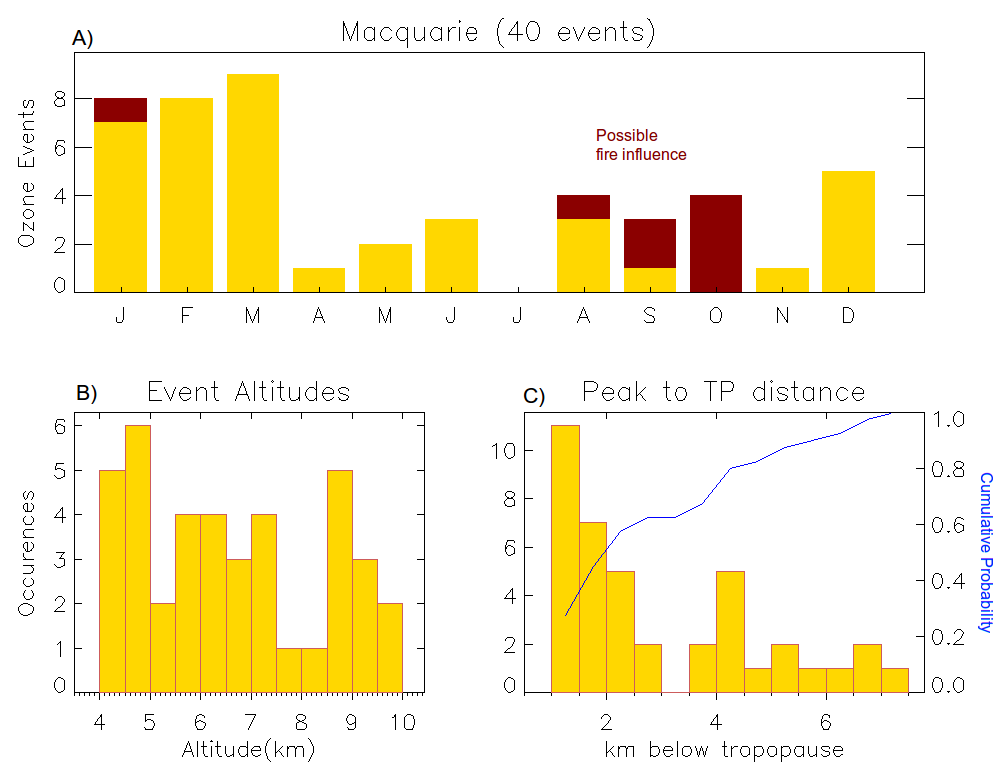
\includegraphics[width=0.8\columnwidth]{Figures/Ozone/Summary_Macq}
      \caption{
      As for Figure~\ref{ch_o3:fig:SummaryMelbourne} except showing the Macquarie Island STT events.%
      }
      \label{ch_o3:fig:SummaryMacquarie}
    \end{figure}

    \begin{figure}[!htbp]
      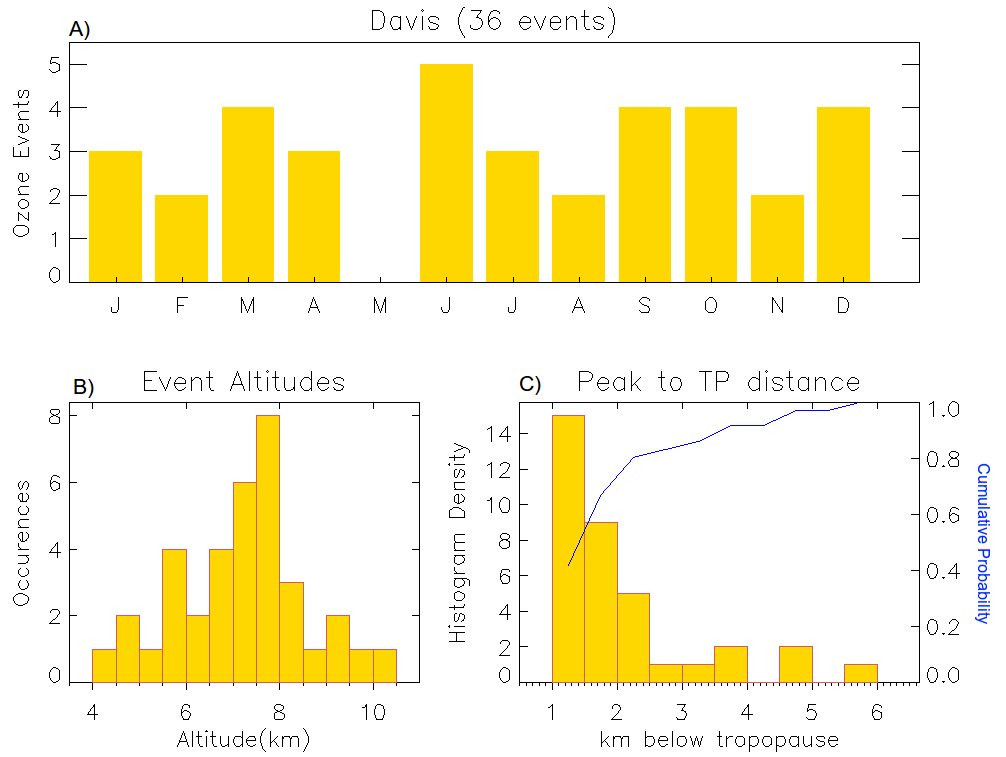
\includegraphics[width=0.8\columnwidth]{Figures/Ozone/Summary_Davi}
      \caption{
      As for Figure~\ref{ch_o3:fig:SummaryMelbourne} except showing the Davis STT events.%
      }
      \label{ch_o3:fig:SummaryDavis}
    \end{figure}
    
%----------------------------------------------------------------------------------------
%	STT impact determination method
%----------------------------------------------------------------------------------------
\section{Stratosphere to Troposphere flux analysis}
  \subsection{Determining a minimum estimate of stratospheric influence}
    Determining how much ozone is transported from the stratophere with only a two dimensional line vector of ozone concentrations is questionable.
    It is assumed that the two dimensional profile is a vertical straight line, which accurately represents the ozone profile in the horizontal dimensions.
    A conservative estimate on stratospheric ozone influence is determined through analysis of the ozone spike above a baseline amount for each column.
    This is a lower bound as it ignores dispersed ozone, baseline enhancements, and any secondary peaks which may also be due to stratospheric transport.
    
    Using our estimate of STT ozone flux (see section \ref{ch_o3:sec:bandpassfilter}) we find a lower bound for the STT ozone flux over each of our three sites, excluding possible fire influence.
    Figure \ref{ch_o3:fig:fluxsummary} shows the climatological mean fraction of total tropospheric column ozone attributed to stratospheric ozone intrusions at each site, on days when an STT event occurs. These flux amounts are calculated after removal of the biomass burning events, although leaving the burning events in changes the means by less than 5\%. The mean fractions of stratospheric ozone are 2--4\%, although the largest fractional ozone in the tropospheric column attributed to stratospheric air exceeds 10\% at all locations.
      

    \begin{figure}[!htbp]
      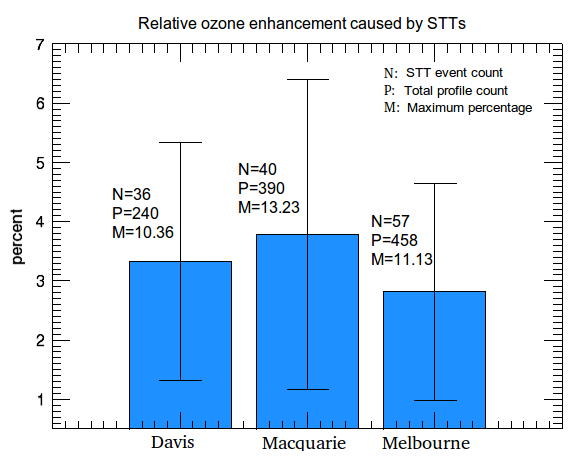
\includegraphics[width=0.8\columnwidth]{Figures/Ozone/FluxSummary_notrans.png}
      \caption{
      Fraction of total tropospheric column ozone attributed to stratospheric air intrusions during STT events. Error bars indicate one standard deviation.%
      }
      \label{ch_o3:fig:fluxsummary}
    \end{figure}
  

%----------------------------------------------------------------------------------------
%	NON-STT Influences
%----------------------------------------------------------------------------------------
\section{Non-STT influences on ozone at southern latitudes}

  \subsection{Fire Plumes}
    Ozone production due to fire smoke plumes is complex and affected by photochemistry, fuel nitrogen load, and atmospheric plume interactions both during transport and at the plume's destination. Ozone precursors include nitrogen oxides ($NO_x = NO + NO_2$) and non methane volatile organic compounds (NMVOCs). Large biomass burning events emit substantial ozone precursors, some of which are capable of being transported far from their origins. NO$_x$ can be transported far downwind due to peroxyacetyl nitrate (PAN) thermal decomposition and this can lead to enhanced ozone far from the source of a fire \citep{Jaffe_2012}.
    
    \citet{Pak2003} show a tropospheric ozone spike over SE Australia in September and using back trajectories suggest that the air masses over Melbourne on this day also passed over South Africa and the higher altitude air also passed through South America.
    The Australian fire season spans most of the year, sweeping southwards as shown in figure and may occasionally affect the ozone columns above either of Macquarie and Melbourne. However, the influence from regional burning is unlikely to affect the ozone concentration above 4~km altitude and most of the smoke from the northern half of Australia is not transported over these sites.
    
    South of 10$^\circ$~S, \citet{Jaffe_2012} estimates that 158 and 54 Tg per year of CO and ozone are emitted emitted and produced respectively by wildfires, with 50\% uncertainty in the ozone production. Due to this possible source of ozone column perturbation, care must be taken to exclude biomass burning influence when analysing STE impacts.

  \subsection{Transport Exclusion}
    \label{ch_o3:sec:airs_fire_filter}
    Biomass burning from the southern tropics (South Africa and South America) is a likely source of interference to and perturbation of ozone measurements. Transported BB plumes influence the southern mid latitudes generally between July and December, as indicated by the methane and CO enhancements ratio ($ \Delta{CH_4}/ \Delta{CO} $) which averages $ 0.31 $ in this time \citep{Pak2003}.
    
    One method of detecting transported emissions influences is through satellite column analysis as done in \citet{Sinha2004}. Smoke plumes from biomass burning create a heavy haze as well as elevated CO concentrations which can be seen from satellites.
  
    Ozone production due to fire smoke plumes is complicated and dependent on many chemical and meteorological factors. Using high CO levels as a proxy in order to determine where fire smoke plumes exist has been done in several studies (eg: \citep{Edwards2003,Sinha2004,Edwards2006,Mari2008}). 
    The AIRS (Atmospheric Infrared Sounder) instrument on board the AQUA satellite records, among other trace gases, column CO. 
    The AQUA satellite overpasses most of the globe twice per day, using the data from the ascending mode swathes at local time 1330 allows some idea of the atmospheric CO on a given day.
    
    In this work a visual inspection of vertical columns of CO (provided by NASA \citep{AIRS3STD}) over the southern hemisphere is used to exclude possible foreign smoke plume influence on the ozone profile at our three sites. 
    Whenever high CO concentrations coincide with sonde detected ozone events it's possible that the tropospheric ozone spike could be due to transported chemicals.
    All occasions where these coincidences occur are removed. Using a scale of 1e18 up to 3.5e18 molecules$/{cm}^2$ can show burning influence  as exemplified in figure \ref{ch_o3:fig:excludedeg}.
    Using 458 ozonesonde profiles over Melbourne, 72 ozone events are detected, of which 15 are discarded as possibly caused by transported fire smoke plumes. 
    Over Macquarie island 48 events are detected from 380 ozonesondes of which 8 are discarded due to possible smoke influence.
    We also include on Figure~\ref{ch_o3:fig:SummaryMelbourne} to Figure~\ref{ch_o3:fig:SummaryDavis} the events which have possible fire influence. These events are concentrated in Spring at melbourne and Macquarie Island.
    
    \begin{figure}[!htbp]
      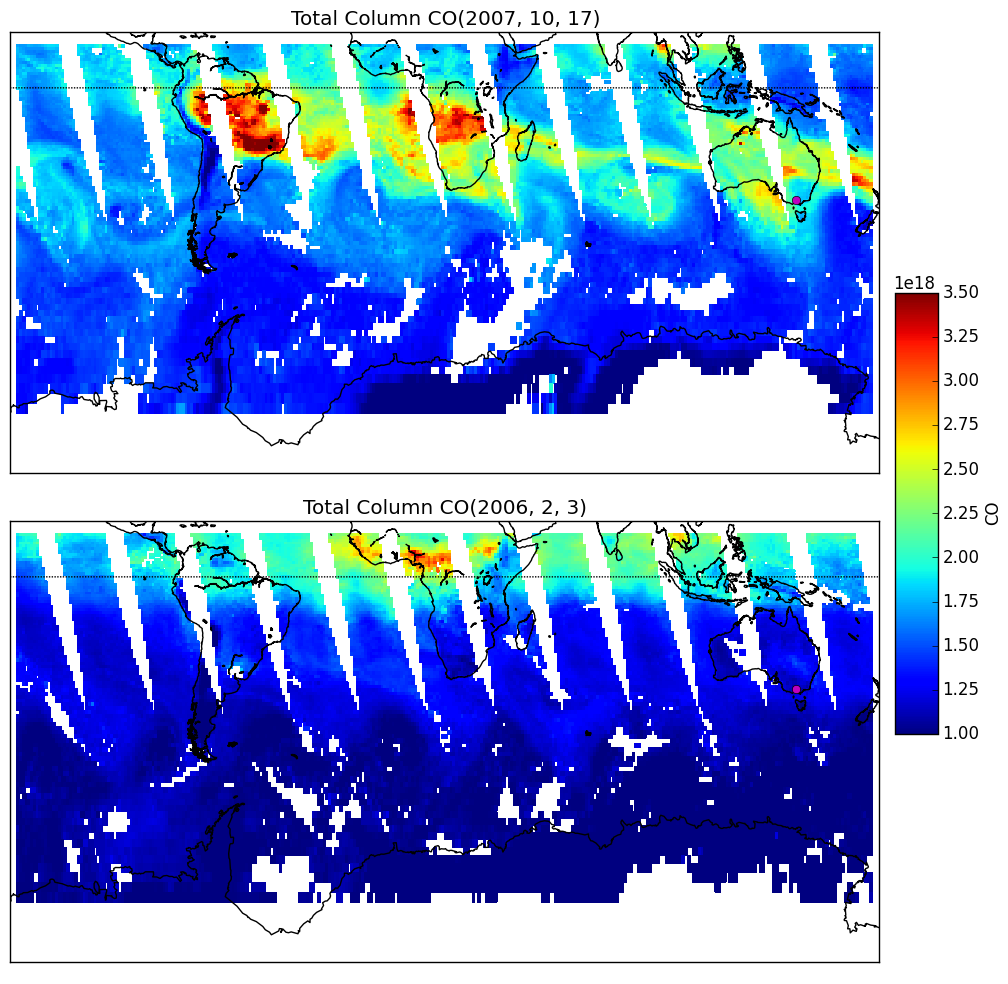
\includegraphics[width=\textwidth]{Figures/Ozone/AIRS_compare.png}
      \caption{AIRS total column CO image showing two days seperate days of swathes. The top panel shows an example of an excluded ozone event which could have been caused by a transported biomass burning plume on October 17th, 2007.}
      \label{ch_o3:fig:excludedeg}
    \end{figure}

  
\section{GEOS-Chem ozonesonde comparison}
  \subsection{Comparing data to GEOS-Chem}
    
    Ozone sondes are useful for looking at specific locations with high resolution, and in this work they provide an estimate of both STT occurence rates and STT ozone flux.
    This information can be used in conjunction with global scale information in order to extrapolate ozone transport over a large area.
    GEOS-Chem is used to simulate the global ozone concentrations.
    In order to check that the model is reasonable, some simple validation is performed comparing sonde data to colocated grid boxes in GEOS-Chem, using the tropospheric columns of ozone as the metrics.
    After the model is validated this way, an extrapolation is performed and the stratospherically sourced ozone is estimated over the latitude range from 30$^{\circ}$S to 75$^{\circ}$S (TODO: Update these numbers with final decided ones, and give a reason).
    Examination of the GEOS-Chem output also gives us an insight as to whether the simulation can be used on its own in order to estimate STT event distribution and magnitude.
    
    A secondary reason to compare ozonesondes to GEOS-Chem is to check that GEOS-Chem chemistry is reasonable and robust. 
    Model validation at any scale increases confidence in the model as well as providing background information to scientists who seek to expand or improve the model.

    GEOS-Chem is a global chemical transport model \citep{Bey2001}, which includes transport, emission, deposition, chemical production and destruction of ozone and 103 other trace gases throughout the troposphere along with stratospheric chemistry, including photolysis. 
    Stratosphere-troposphere coupling is calculated using the stratospheric unified chemistry extension (UCX) \citep{Eastham2014}, which includes a further 28 trace gases.
    Transport is driven by assimilated meteorological fields from the Goddard Earth Observing System (GEOS-5) maintained by the Global Modeling and Assimilation Office (GMAO) at NASA.
  
    GEOS-Chem values used within this chapter are based on a simulation using UCX from 2004-2013, with 2004 used as a spinup year.
    The simulation uses 2$^{\circ}$ latitude by 2.5$^{\circ}$ longitude horizontal resolution, with 72 vertical levels from the surface to 0.1~hPa.
    Biogenic emissions of organic chemicals are determined by the Model of Emissions of Gases and Aerosols from Nature (MEGAN) version 2.1 extended by Guenther et al \citep{Guenther2012}.
    Anthropogenic emissions are given by the Emissions Database for Global Atmospheric Research (EDGAR) version 4.2.
    Our simulation was modified from the standard v10-01 to a fix a bug in the treatment of the Total Ozone Mapping Spectrometer (TOMS) satellite data used to calculate photolysis (see TODO:wiki entry for fix or supplementary).
    GEOS-Chem uses measurements from the Total Ozone Mapping Spectrometer (TOMS) satellite instrument with the Fast-JX photolysis rate solver customised for use in the stratosphere in order to simulate stratospheric ozone photolysis.
    
  \subsection{Determining tropospheric ozone from GEOS-Chem}
    GEOS-Chem allows certain diagnostics, along with any tracer, to be output at higher temporal resolution for a list of latitude and longitude based boxes.
    Storing output every six hours allows an examination of vertical profiles at a list of specific latitudes and longitudes during both day and night.
    Using the ozone mixing ratio ($C_{O_3}$ in molecules O$_3$ per molecule of air) at 72 vertical layers and the air density (N$_{Air}$ in molecules per cm$^3$), provides us with the ozone density profile (N$_{O_3}$):
    \begin{equation*}
     N_{O_3}[z] = C_{O_3}[z] \times N_{Air}[z]
    \end{equation*}
    where z is the vertical level index.
    
    In order the determine the tropospheric ozone column ($TC_{O_3}$ in molecules cm$^{-2}$), we first use the modelled tropopause pressure (TPP in hPa) to determine where the troposphere ends.
    The TPP is used to determine how many vertical levels exist in the troposphere.
    This is done through comparison with the pressure edges of each level.
    The linear fraction (frac) of the level containing the TPP is then obtained from the pressure edges below and above the TPP (pb and pa respectively):
    \begin{equation*}
     frac = \frac{p_b - TPP}{p_b-p_a}
    \end{equation*}
    
    At every time step, using the above calculations along with the layer heights (H in cm), the tropospheric ozone (TVC$_{O_3}$ in molecules cm$^{-2}$) is determined as follows: $N_{O_3}[z] \times H[z]$ gives the vertical profile of molecules cm$^{-2}$, which is then summed up to the TPP:
    \begin{equation*}
     TVC_{O_3} = \Sigma_{z=0}^{z_{TPP}-1} \left( N_{O_3}[z] \times H[z] \right) + frac \times N_{O_3}[z_{TPP}] \times H[z_{TPP}]
    \end{equation*}
    where $z_{TPP}$ is the index of the level containing the tropopause.
    
    Figure \ref{ch_o3:fig:StationSeriesGEOSChem} shows the time series of tropospheric ozone (TVC$_{O_3}$) simulated over our three stations from January 1 2005 to January 1 2011.
    Coplotted as stars are the measured tropospheric ozone columns calculated using the GPH and ozone partial pressure recorded by the ozone sondes.
    The GEOS-Chem simulation uses horizontal resolution of 2$^{\circ}$ latitude by 2.5$^{\circ}$ longitude, and the profiles and totals above each site are actually the average over the horizontal area containing each station.
    There is good aggreement between the modelled tropospheric ozone columns and the measurements, with matching seasonal cycles and magnitude.
    All three sites have a discernable yearly cycle, with Davis having the least spread as well as the greatest outliers.
    These outlying tropospheric ozone columns all occur during the July to September months (TODO: reasons for why? simulated summer turbulence?).
    Both Macquarie Island and Melbourne have more variance in their tropospheric columns.
    For both sites the data is more spread out over the winter months.
    This variability is shown in more detail in figure \ref{ch_o3:fig:YearlyCyclGEOSChem}.
    
    Figure \ref{ch_o3:fig:YearlyCyclGEOSChem} shows the yearly averaged tropospheric ozone column over our three sites.
    This figure is created using the monthly averages along with their standard deviations.
    Melbourne has the largest tropical ozone column throughout the year, with a summer peak and winter minimum.
    Davis has the lowest ozone levels, with an opposite seasonal cycle to that of Melbourne.
    At Macquarie Island, there is a more subtle seasonal cycle, with slightly more ozone occuring in winter than in summer.
    
    \begin{figure}[!htbp]
      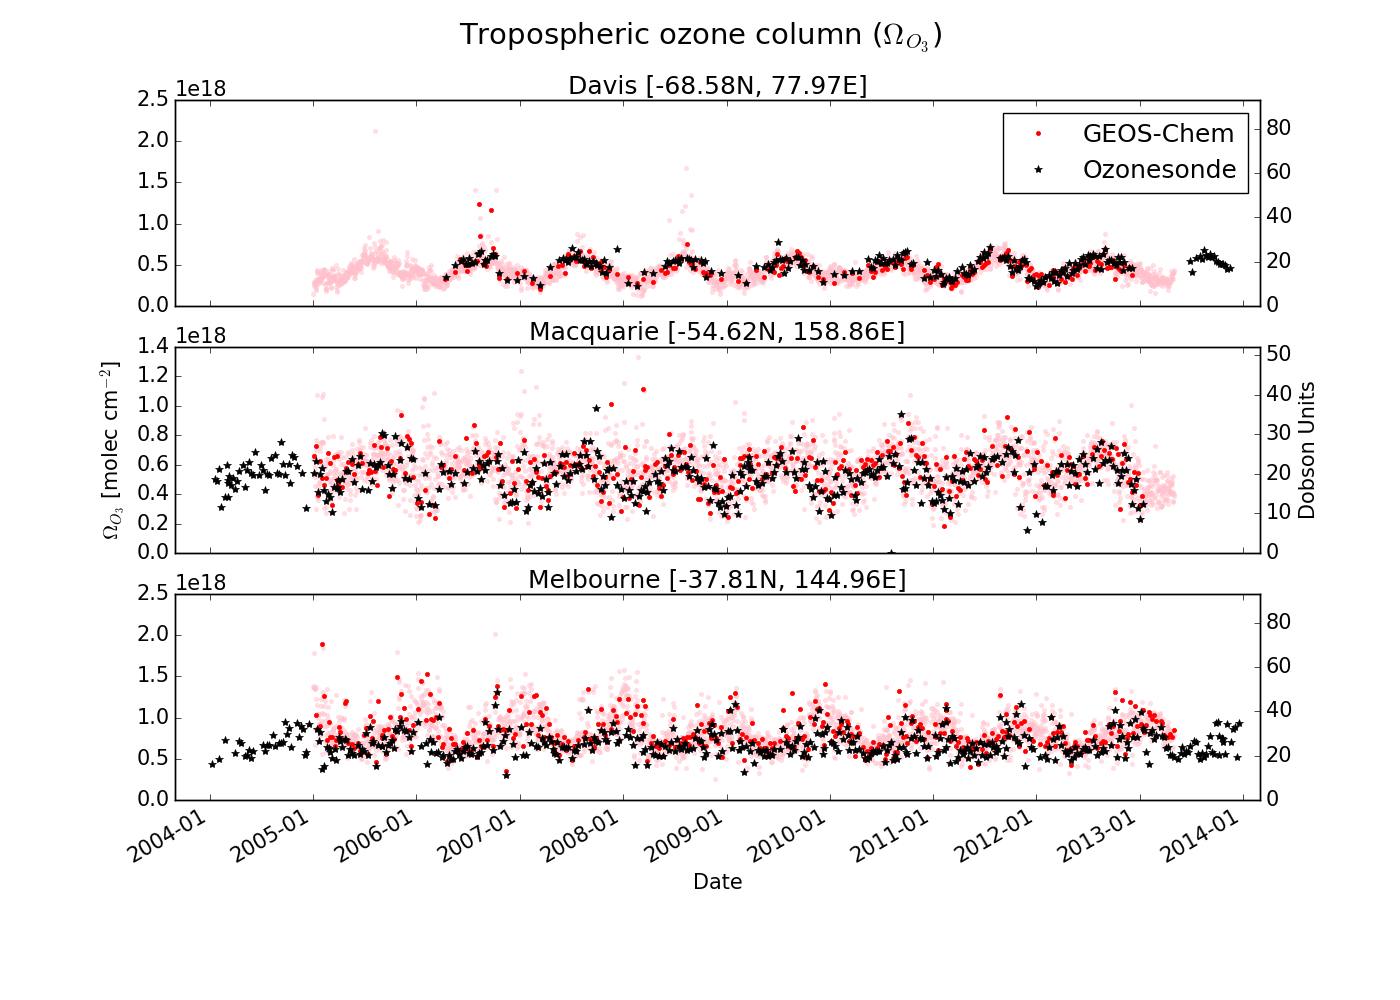
\includegraphics[width=\textwidth]{Figures/Ozone/StationSeries.png}
      \caption{Tropospheric ozone in molecules cm$^{-2}$ every six hours simulated by GEOS-Chem (blue line) from January 1 2004 until December 31 2010. The ozonesonde calculated tropospheric ozone columns are shown as stars, each representing one measurement. }
      \label{ch_o3:fig:StationSeriesGEOSChem}
    \end{figure}
    
    \begin{figure}[!htbp]
      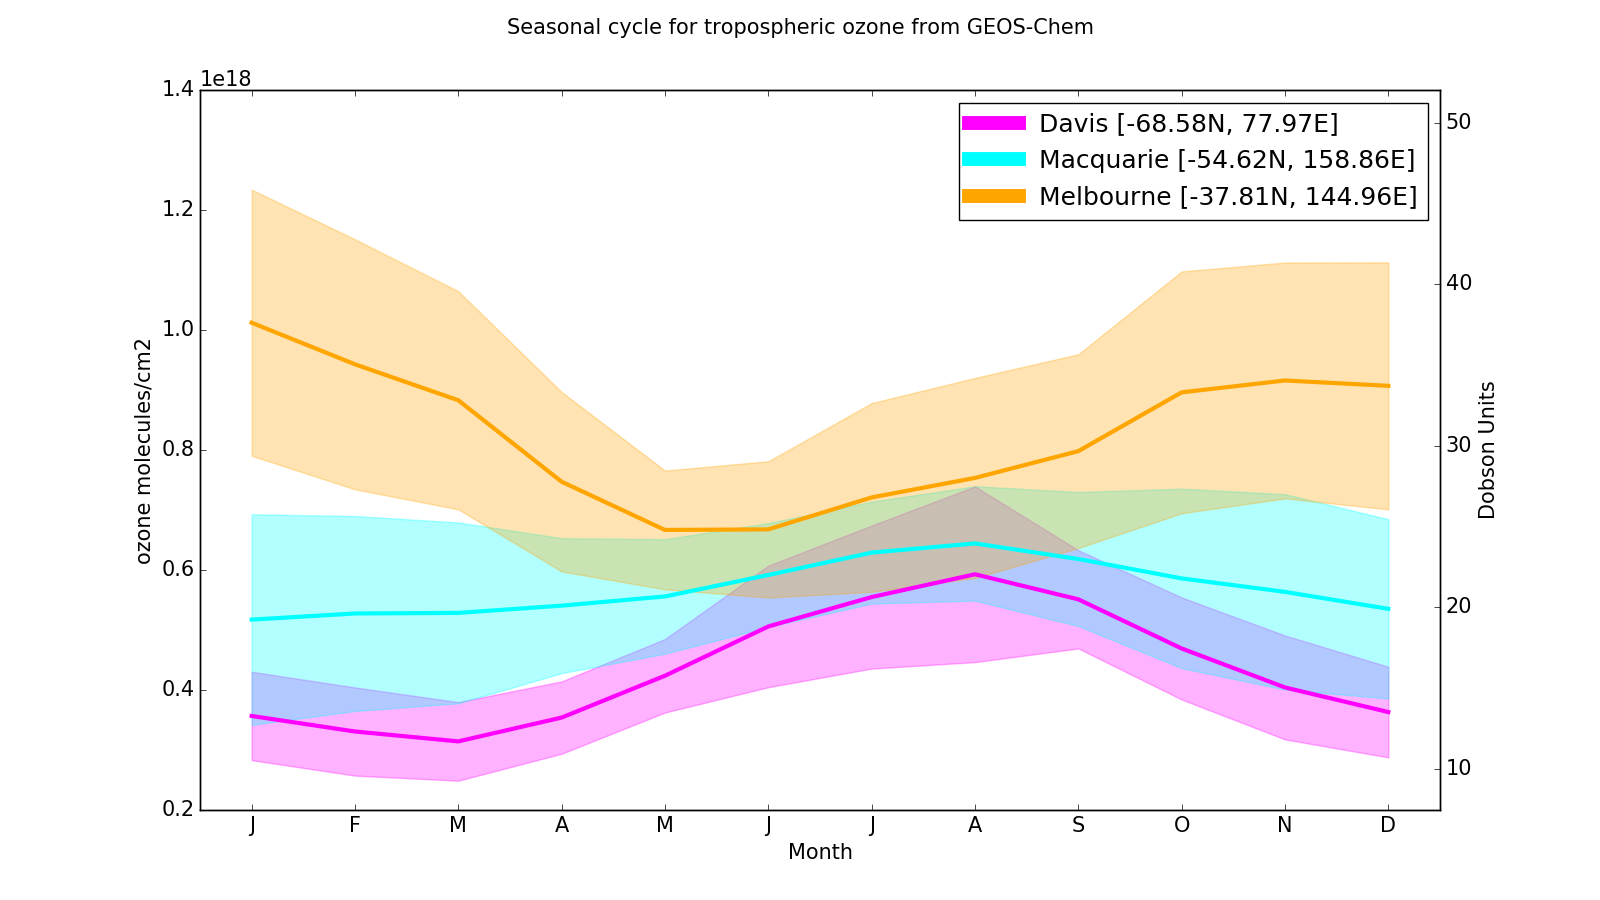
\includegraphics[width=\textwidth]{Figures/Ozone/Yearly_cycle.png}
      \caption{Tropospheric ozone in molecules cm$^{-2}$ seasonal cycle simulated by GEOS-Chem from January 1 2004 until December 31 2010. The monthly averages are taken for each year and the mean plotted with one standard deviation shaded.}
      \label{ch_o3:fig:YearlyCyclGEOSChem}
    \end{figure}
    
  \subsection{Ozone profiles compared with GEOS-Chem}
    GEOS-Chem provides 72 vertical levels of data, of which about 30 will be in the troposphere.
    The ozone sondes generally have more than 100 vertical levels below the tropopause.
    Interpolating the vertical levels to a standard set of altitudes allows an examination of both the mean ozone profils and the standard deviation at each altitude.
    For each of the GEOS-Chem and sonde vertical profiles, the data is interpolated to 100 points between 0 and 14~km, at which the mean and standard deviation is determined for each month.
    
    Figures \ref{ch_o3:fig:GEOSChemMonthlyProfilesDavis}-\ref{ch_o3:fig:GEOSChemMonthlyProfilesMelbourne} show the simulated monthly averaged ozone profile at Davis, Macquarie Island, and Melbourne respectively.
    The shaded areas show $\pm 1$ standard deviation, while the horizontal dotted line shows the mean tropopause height.
    The effect of pollution and mainland influence can be seen over Melbourne, mostly during the summer months (DJF), as the lower altitudes have increased ozone mean as well as more variance.
    Also the yearly cycle of tropopause height for each site is noticible, and it matches the ozonesonde recorded tropopause seasonal cycle.
    Examining the mean profiles at particular hours only shows a noticible difference (not shown unless someone tells me to) over Melbourne, the other two stations are very similar regardless of which hour we examine.
    
    \begin{figure}[!htbp]
      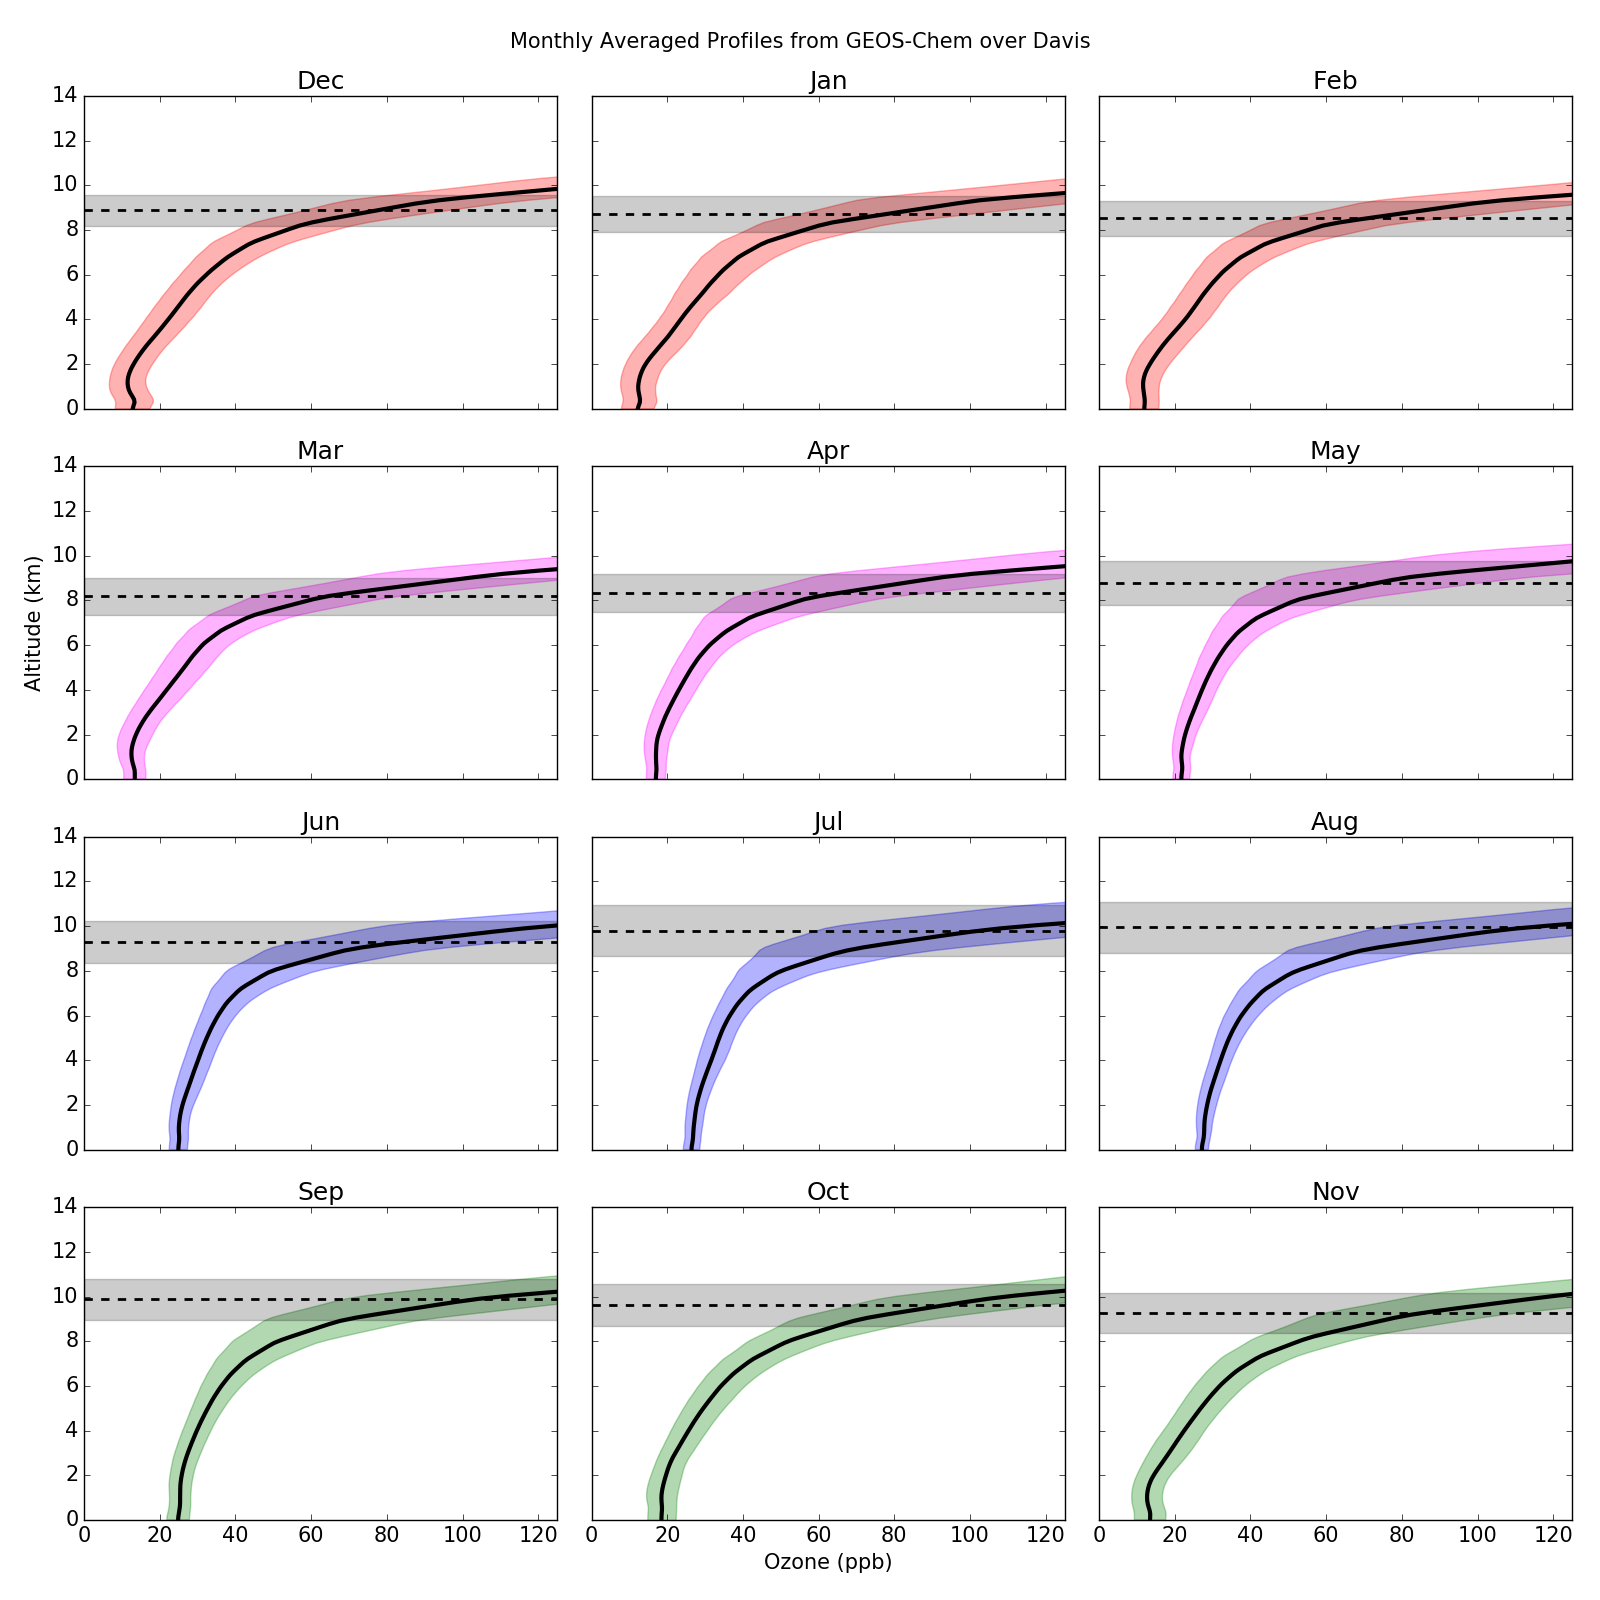
\includegraphics[width=\textwidth]{Figures/Ozone/Davis_GC_monthprofiles.png}
      \caption{Tropospheric ozone (ppb) simulated by GEOS-Chem over Davis from January 1 2004 until December 31 2010, averaged monthly.
      Horizontal dotted line shows the mean tropopause height, shaded areas show one standard deviation.}
      \label{ch_o3:fig:GEOSChemMonthlyProfilesDavis}
    \end{figure}
    \begin{figure}[!htbp]
      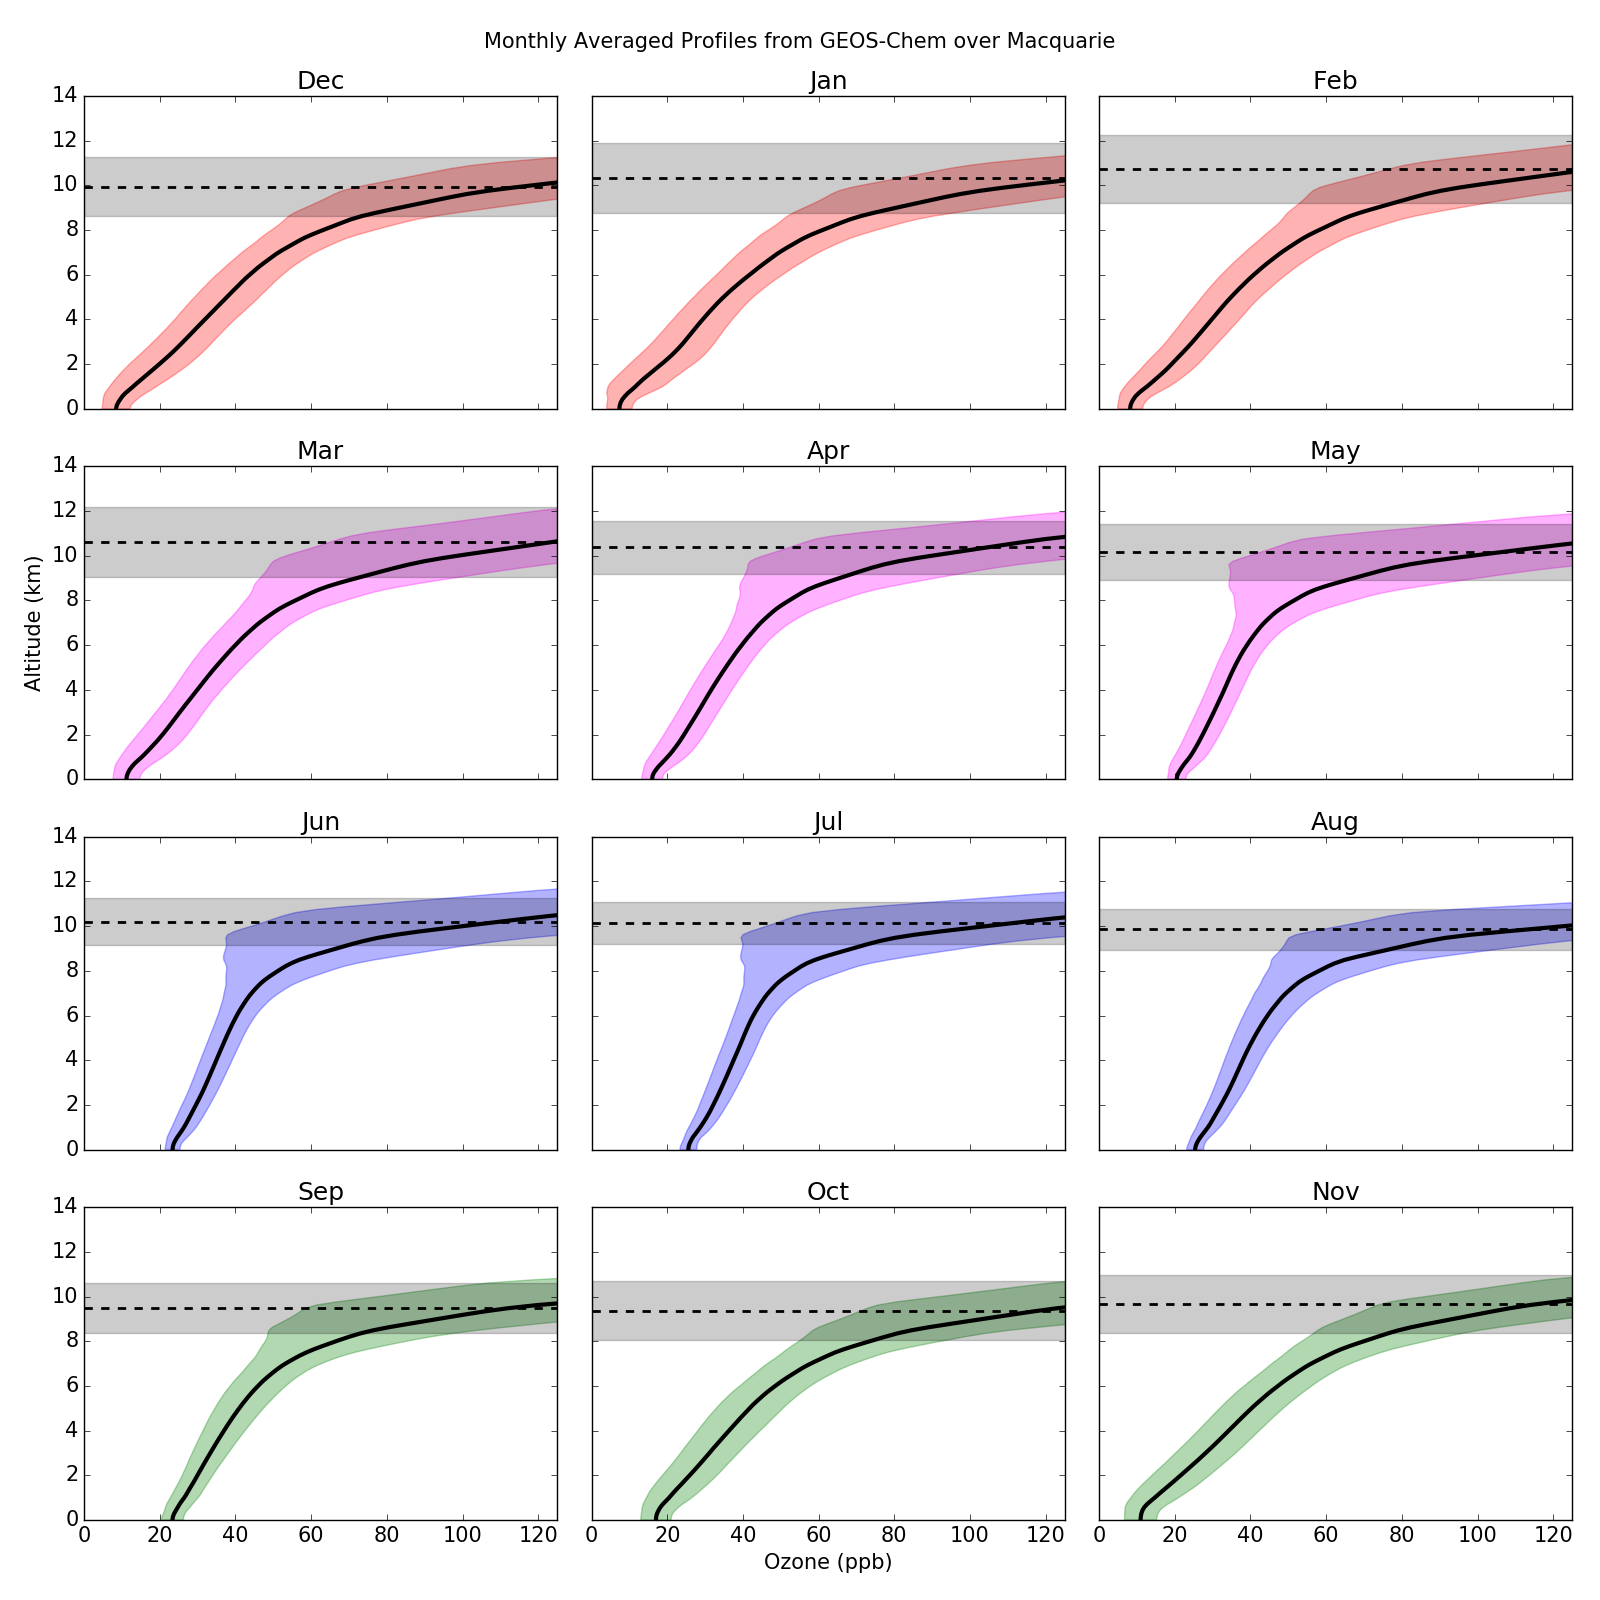
\includegraphics[width=\textwidth]{Figures/Ozone/Macquarie_GC_monthprofiles.png}
      \caption{As figure \ref{ch_o3:fig:GEOSChemMonthlyProfilesDavis} over Macquarie Island.}
      \label{ch_o3:fig:GEOSChemMonthlyProfilesMacquarie}
    \end{figure}
    \begin{figure}[!htbp]
      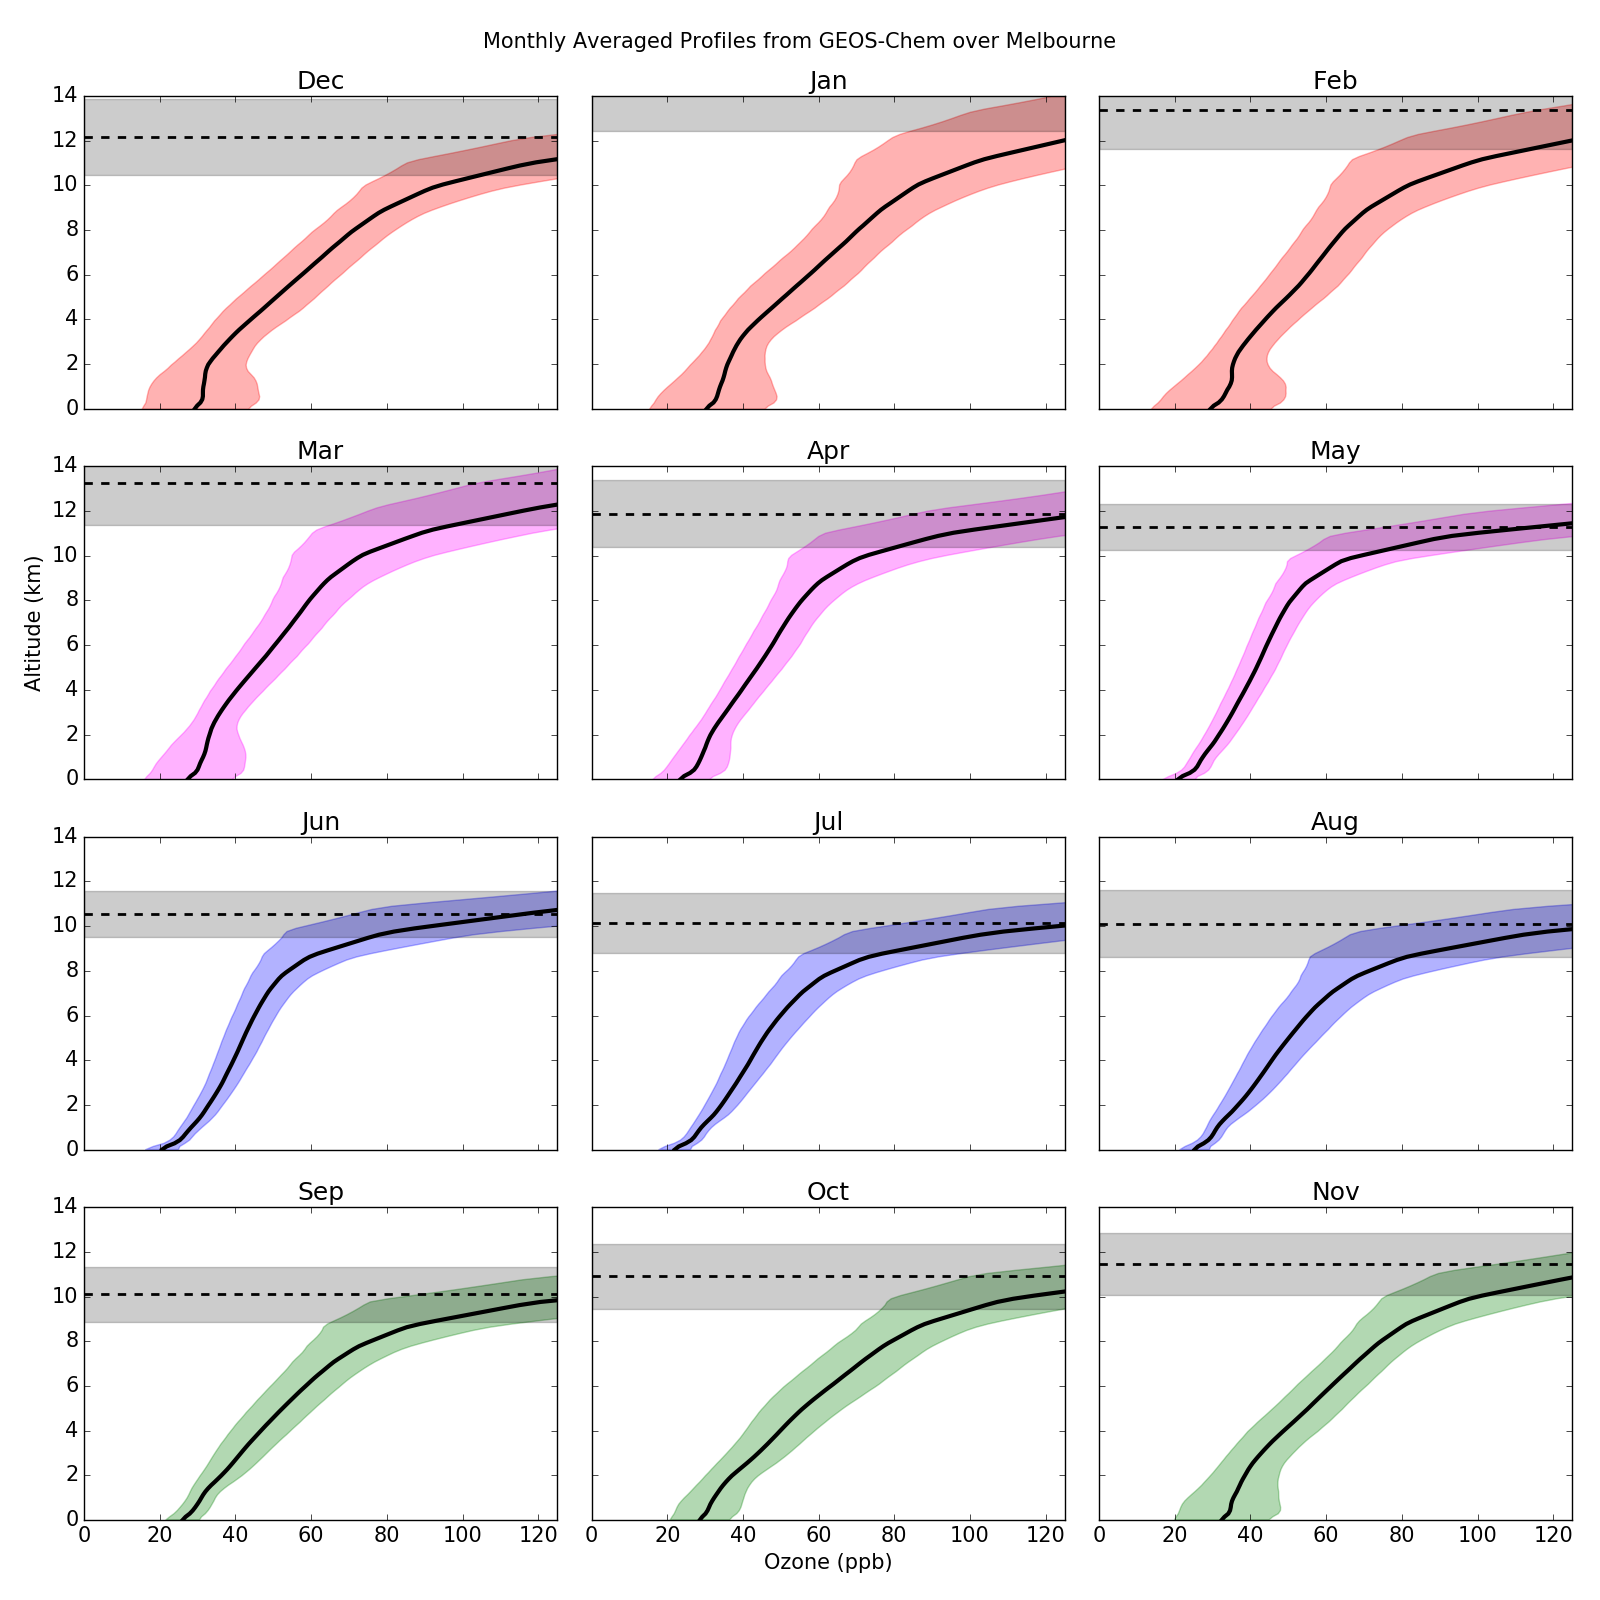
\includegraphics[width=\textwidth]{Figures/Ozone/Melbourne_GC_monthprofiles.png}
      \caption{As figure \ref{ch_o3:fig:GEOSChemMonthlyProfilesDavis} over Melbourne.}
      \label{ch_o3:fig:GEOSChemMonthlyProfilesMelbourne}
    \end{figure}
    
    Figures \ref{ch_o3:fig:SondeMonthlyProfilesDavis}-\ref{ch_o3:fig:SondeMonthlyProfilesMelbourne} show the measured monthly averaged ozone profile at Davis, Macquarie Island, and Melbourne respectively.
    At Davis, the tropopause level slightly lower in summer and autumn than in winter and spring.
    This yearly variation matches the tropopause heights simulated by GEOS-Chem, and is opposite to the yearly tropopause height cycle seen in Melbourne.
    Macquarie does not have a seasonal cycle of tropopause heights, which agrees with the GEOS-Chem profiles, although the GEOS-Chem tropopause heights are slightly higher at all months.
    For Melbourne the gradient of increasing ozone with increasing altitude is stronger in the GEOS-Chem output than the sonde measurements.
    
    \begin{figure}[!htbp]
      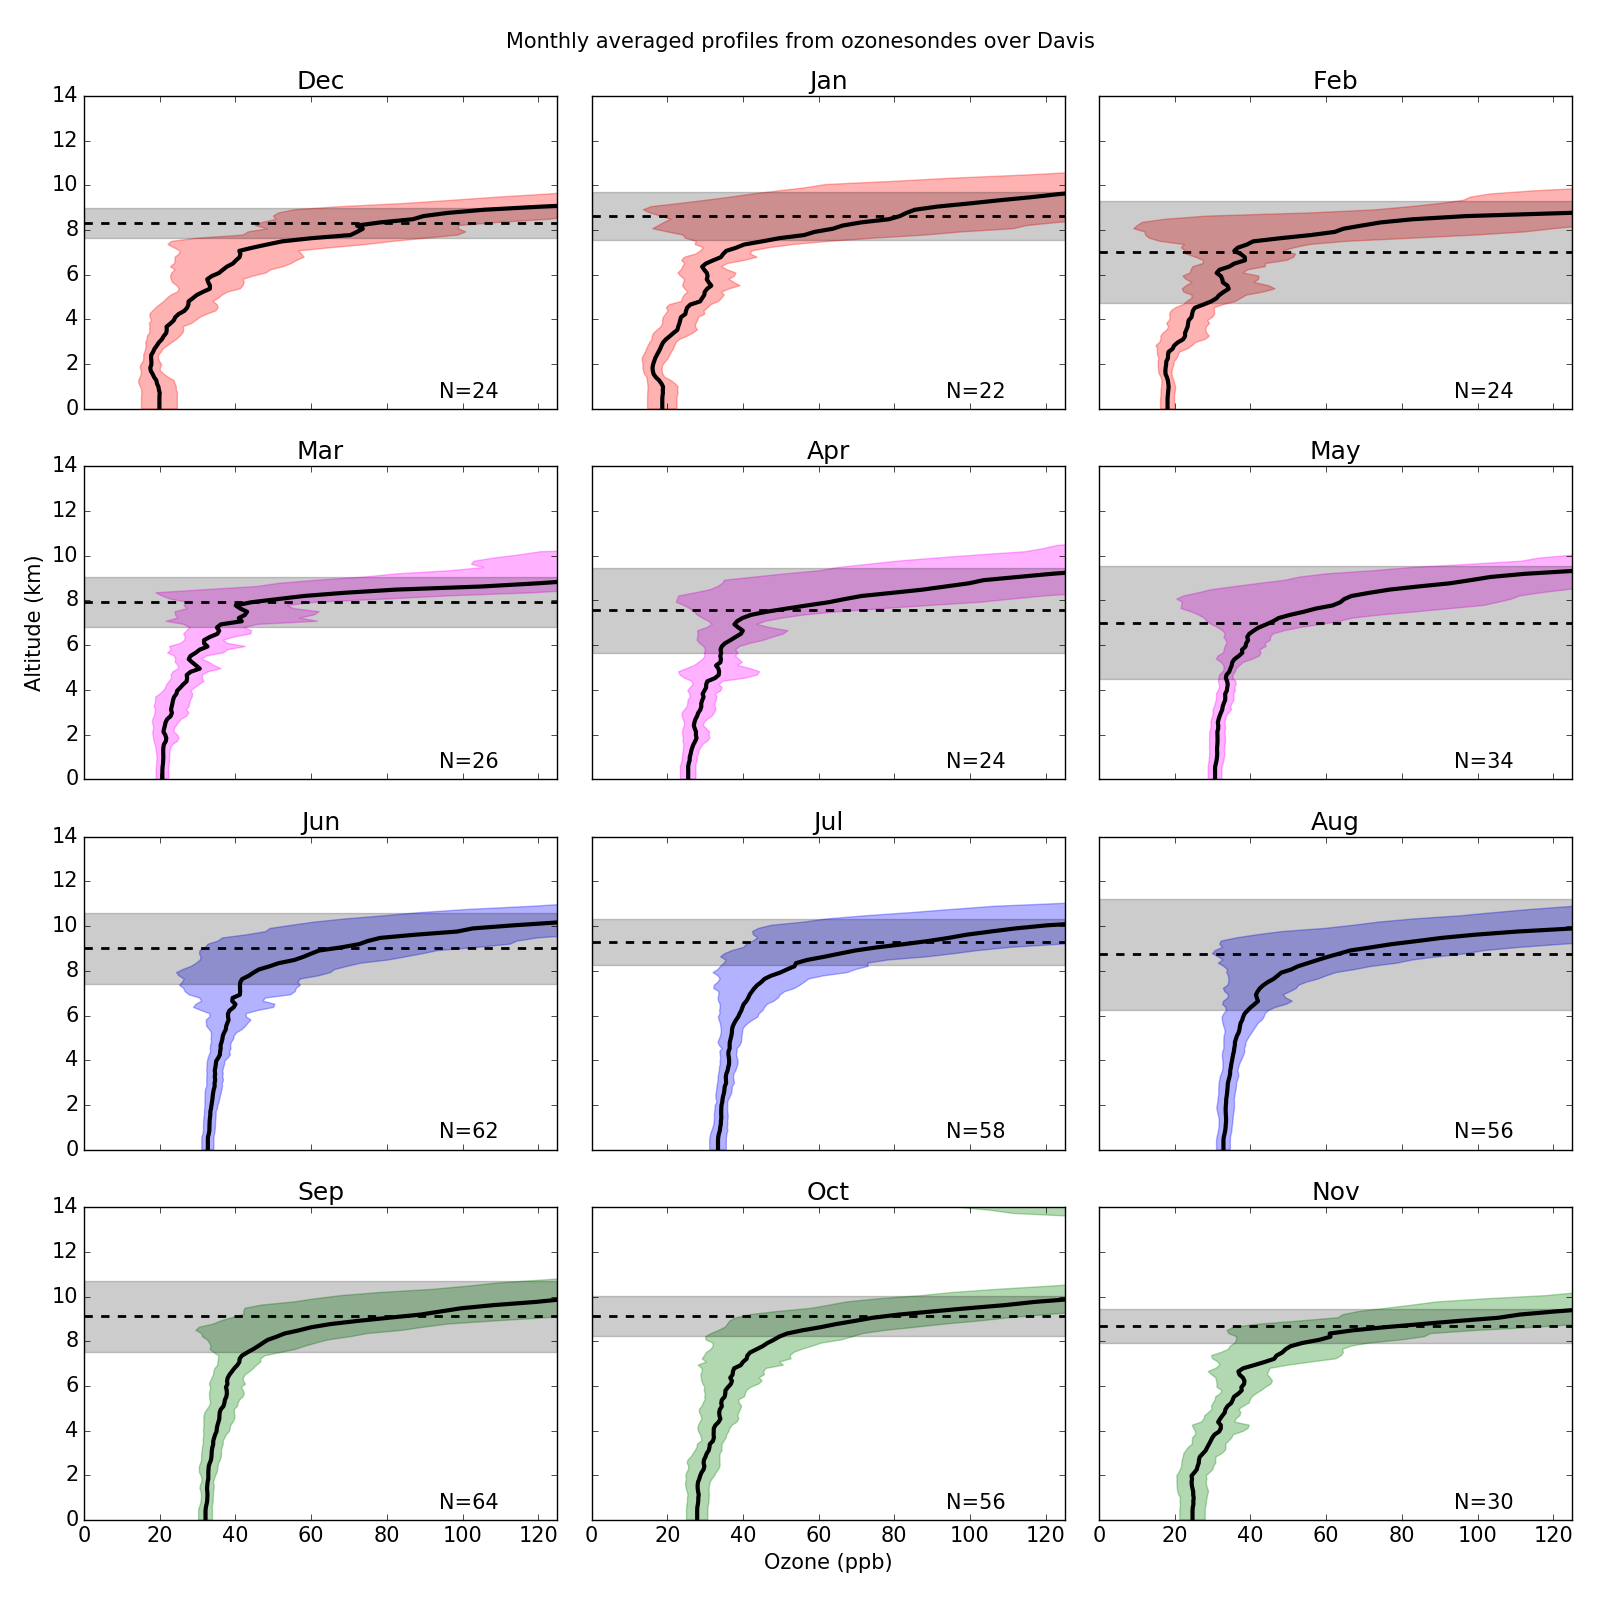
\includegraphics[width=\textwidth]{Figures/Ozone/Davis_sonde_monthprofiles.png}
      \caption{Tropospheric ozone (ppb) measured by ozone sonde over Davis, averaged monthly.
      Horizontal dotted line shows the mean tropopause height, shaded areas show one standard deviation.}
      \label{ch_o3:fig:GEOSChemMonthlyProfilesDavis}
    \end{figure}
    \begin{figure}[!htbp]
      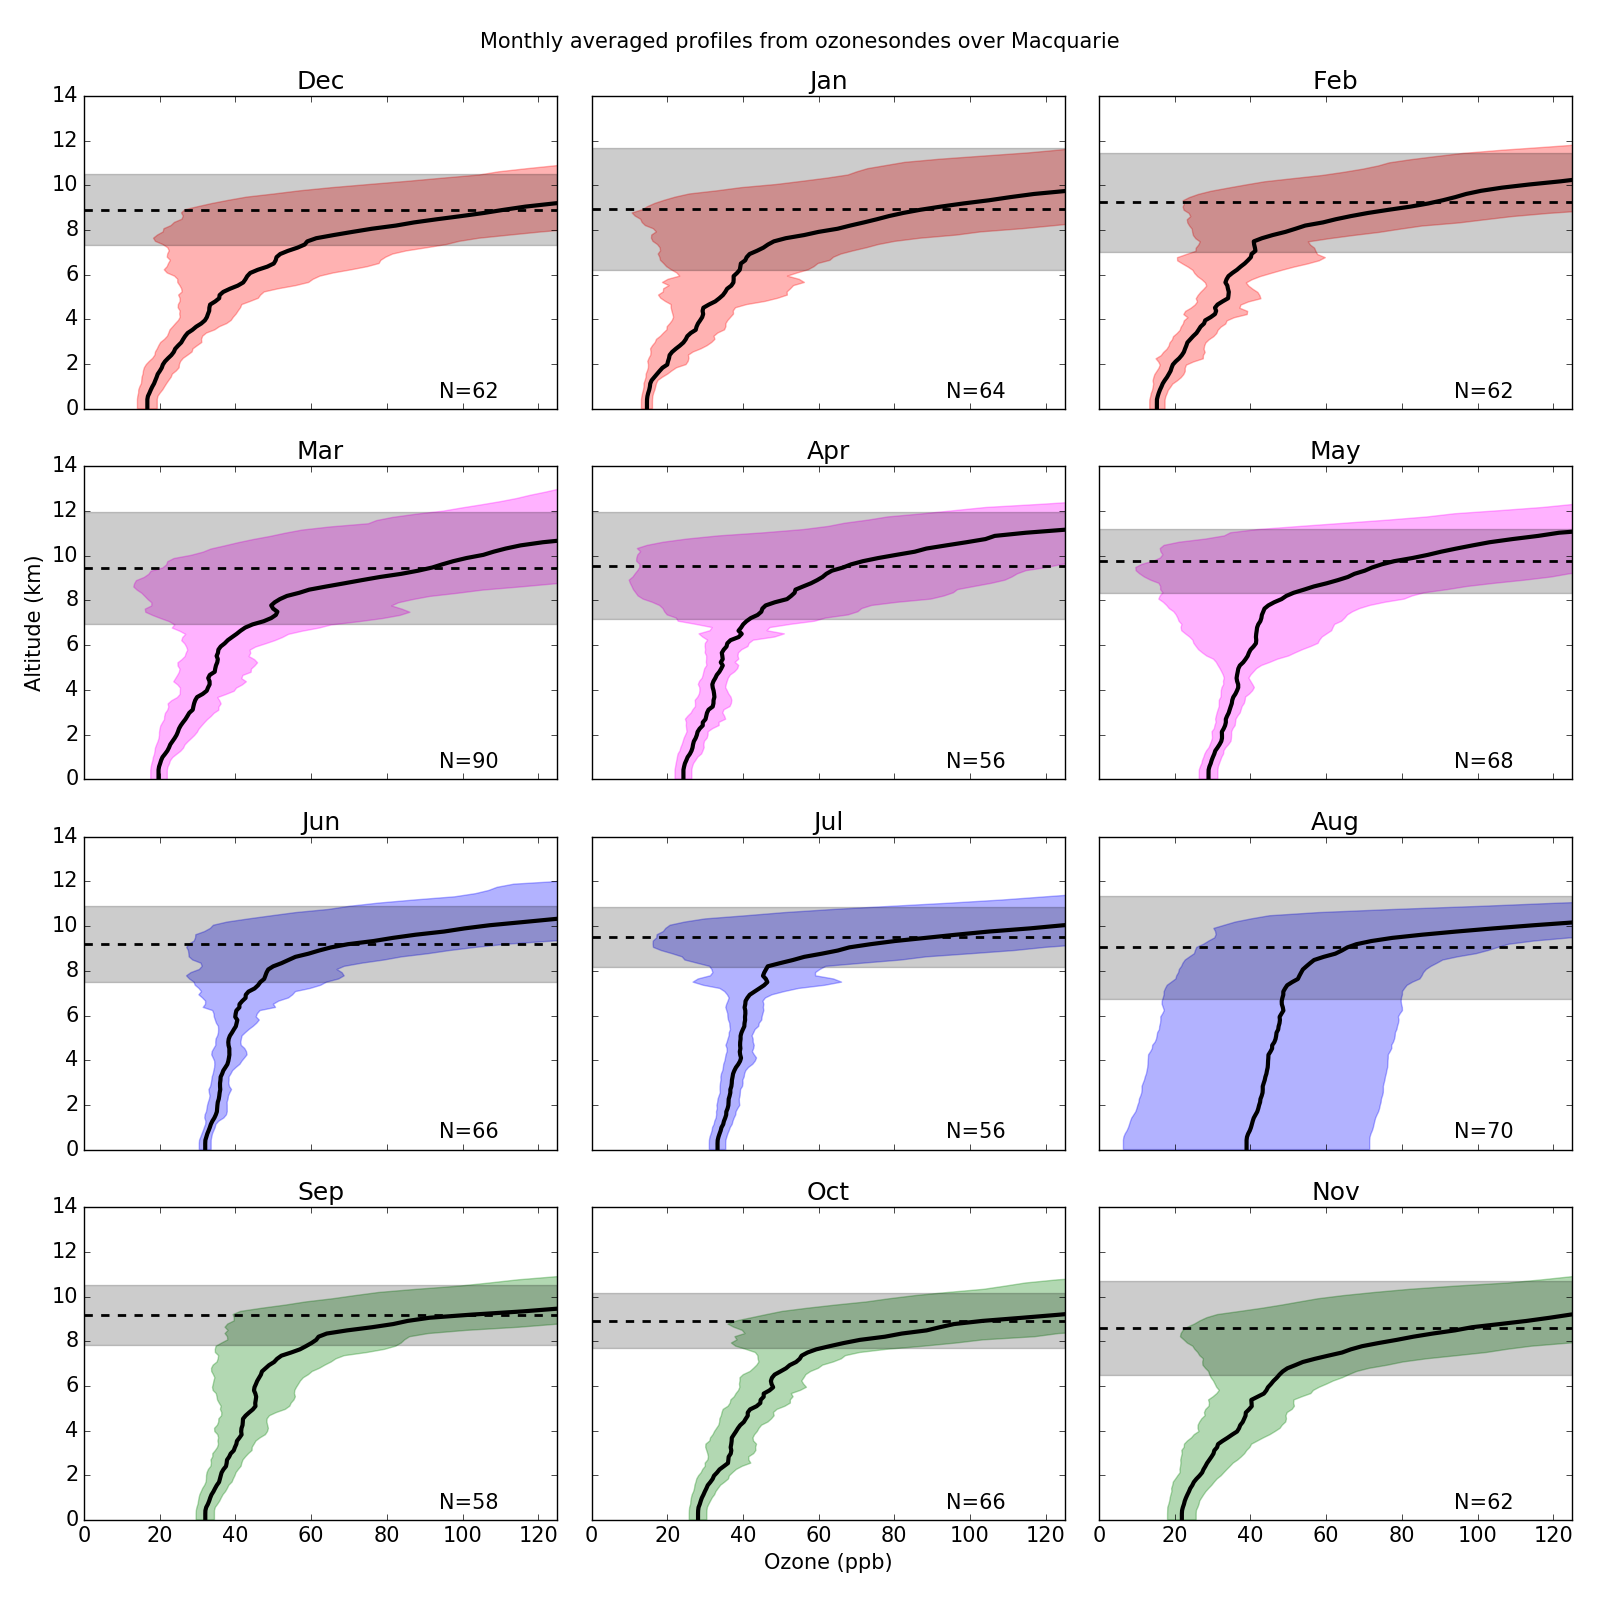
\includegraphics[width=\textwidth]{Figures/Ozone/Macquarie_sonde_monthprofiles.png}
      \caption{As figure \ref{ch_o3:fig:GEOSChemMonthlyProfilesDavis} over Macquarie Island.}
      \label{ch_o3:fig:GEOSChemMonthlyProfilesMacquarie}
    \end{figure}
    \begin{figure}[!htbp]
      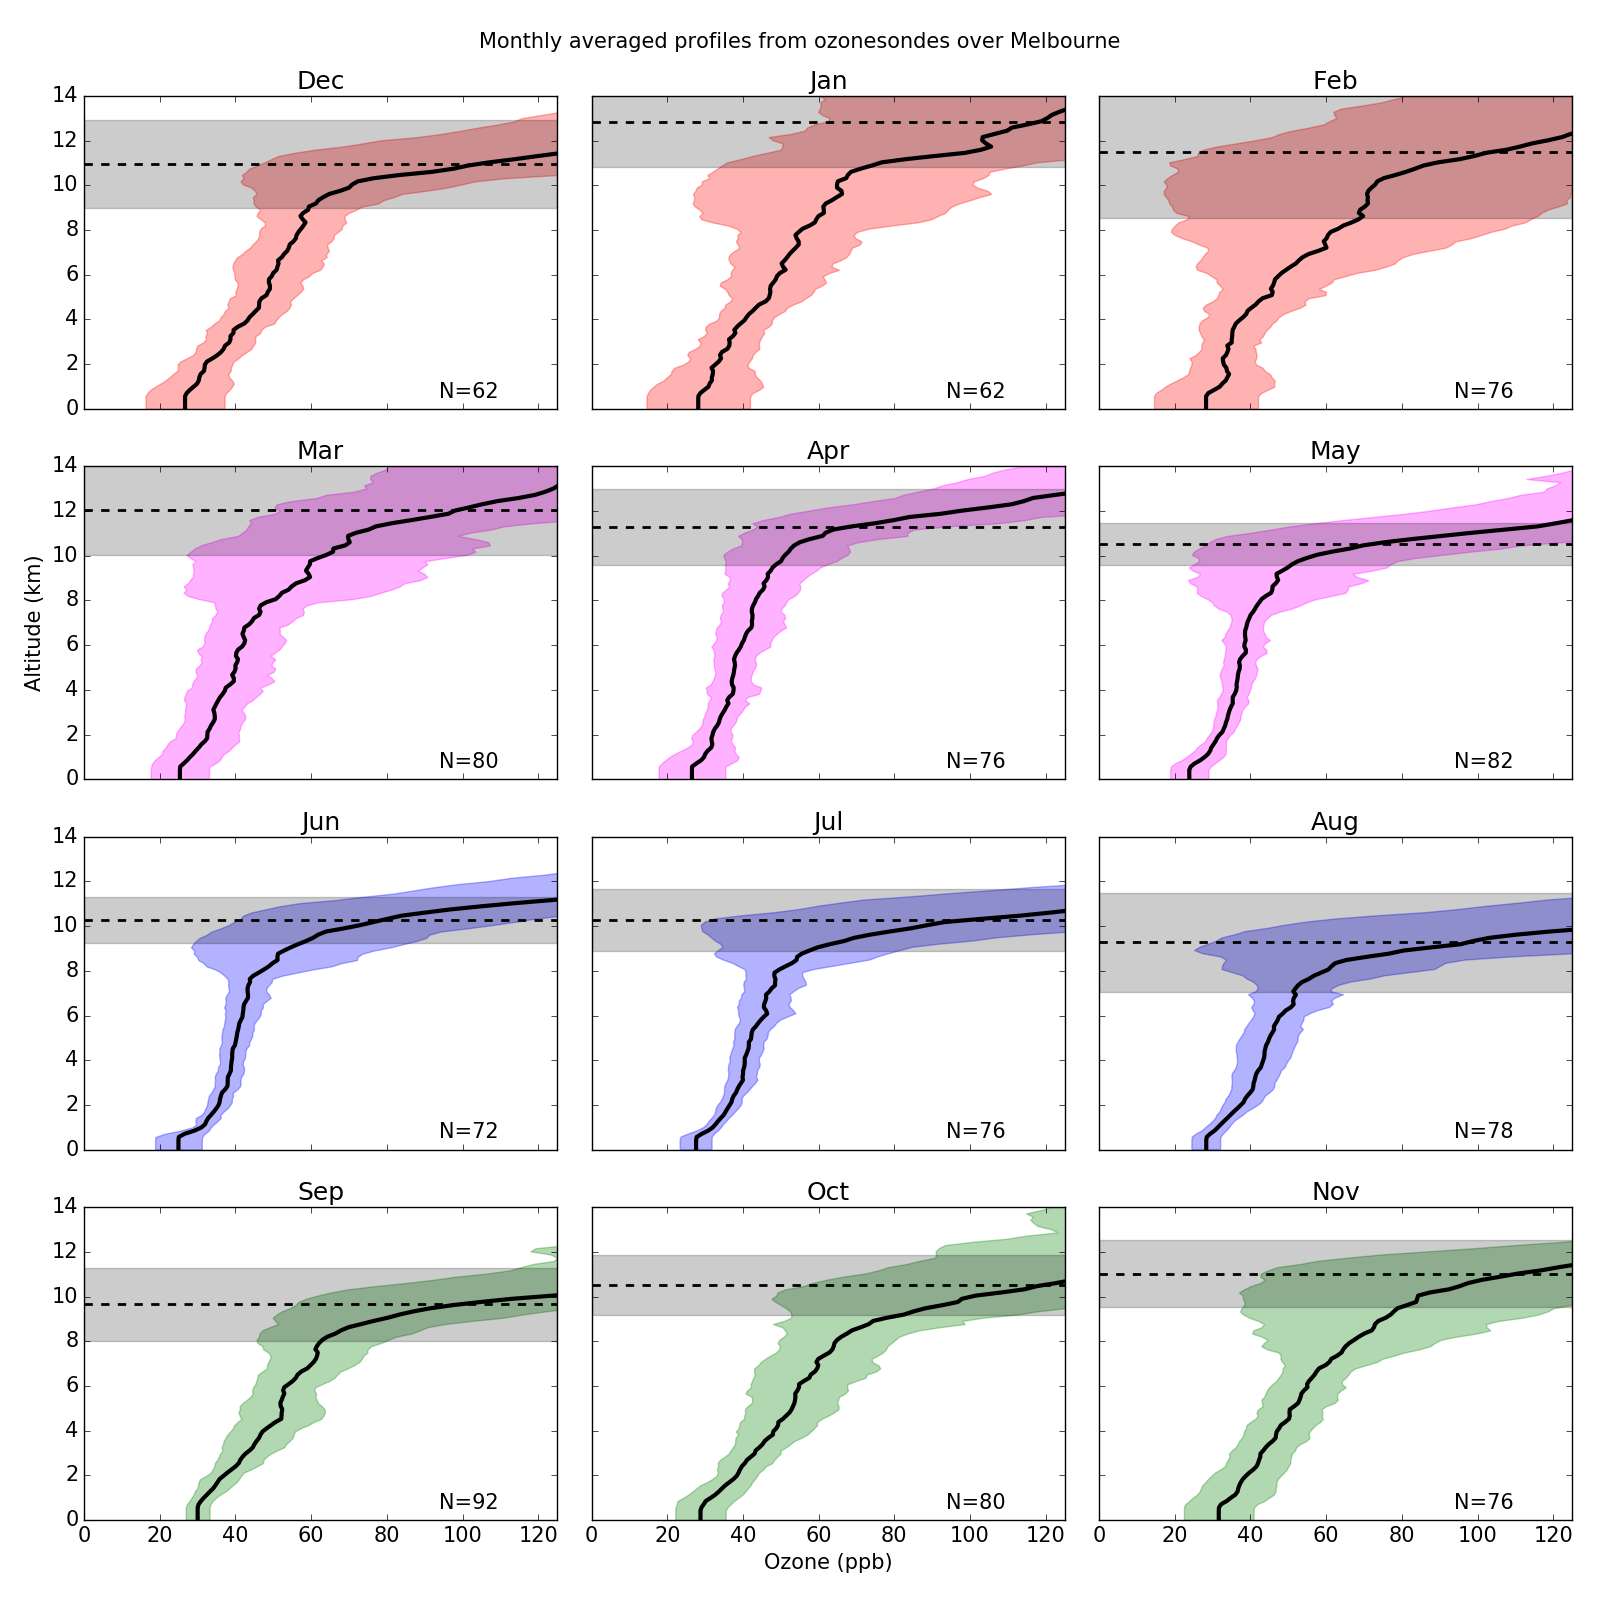
\includegraphics[width=\textwidth]{Figures/Ozone/Melbourne_sonde_monthprofiles.png}
      \caption{As figure \ref{ch_o3:fig:GEOSChemMonthlyProfilesDavis} over Melbourne.}
      \label{ch_o3:fig:GEOSChemMonthlyProfilesMelbourne}
    \end{figure}
    
    Although GEOS-Chem reasonably matches the ozonesonde tropospheric ozone column, it does not have the resolution required to capture STTs.
    Figure \ref{ch_o3:fig:event_profile_comparison} shows the best and worst comparisons of ozone profiles up to 14~km between the ozonesondes and GEOS-Chem.
    The model output is shown in red, and is the average over 2$^{\circ}$ latitude by 2.5$^{\circ}$ longitude which contain the respective sonde release site.
    The vertical resolution from GEOS-Chem is too low to allow detection of STTs, there are roughly 30 vertical levels up to the tropopause, while sondes have upwards of 100.
    These best and worst examples are determined qualitatively, and are shown as examples of the model-measurement differences.
    
    \begin{figure}[!htbp]
      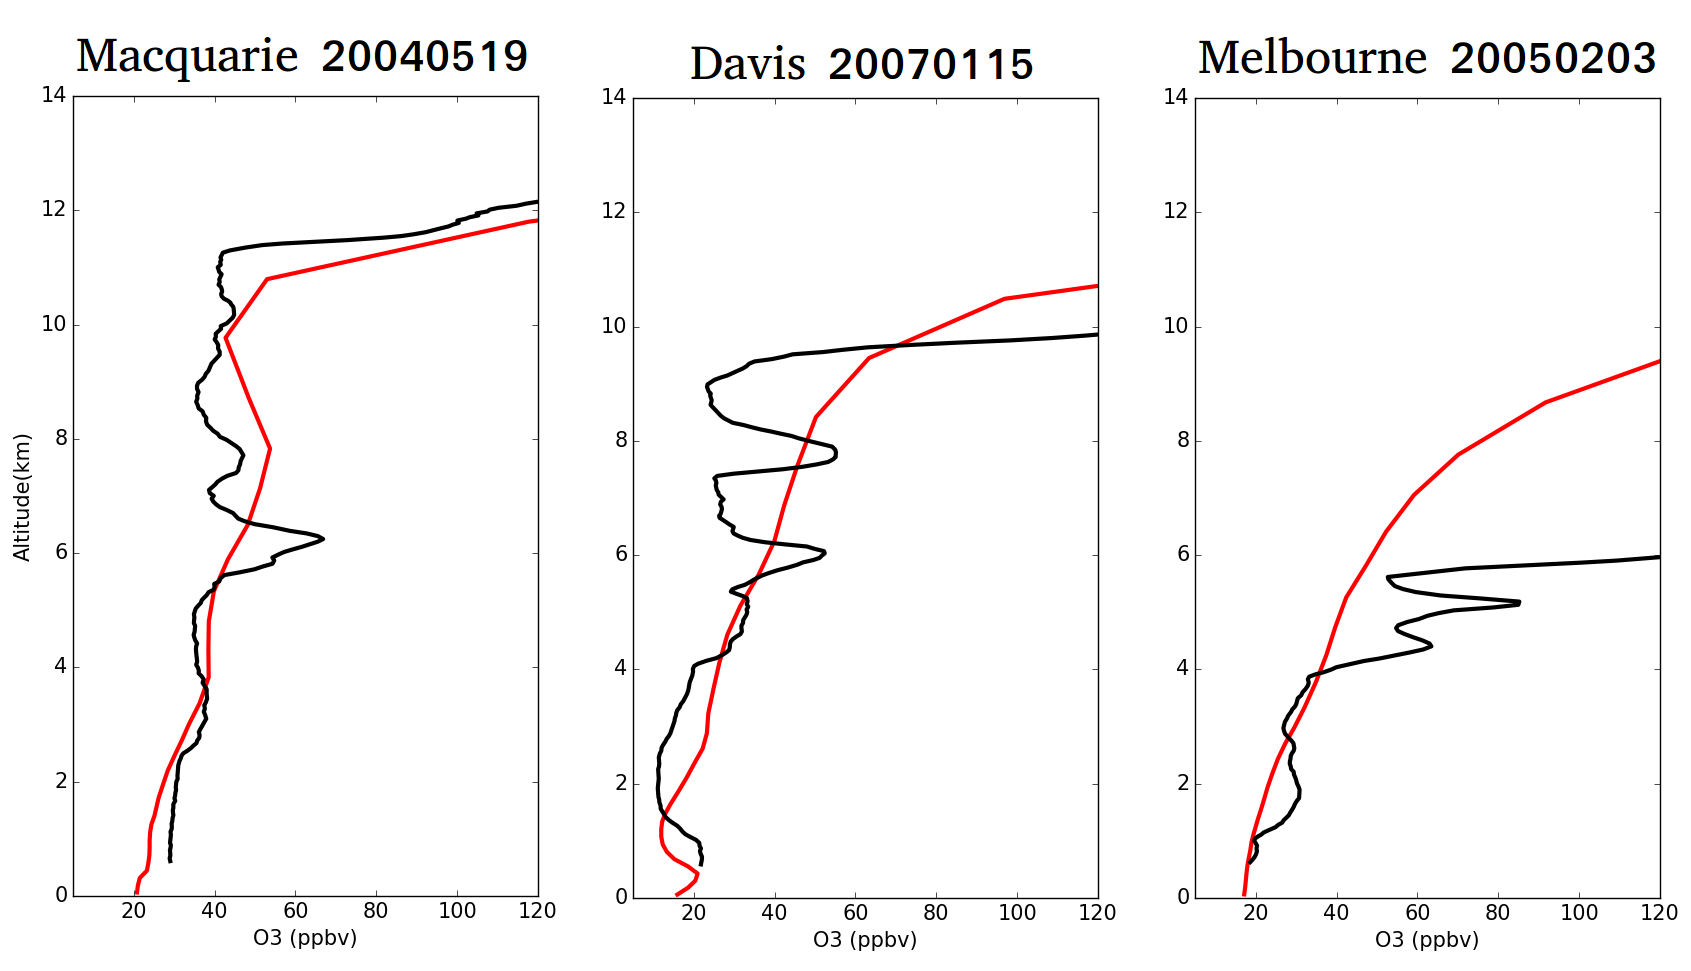
\includegraphics[width=\textwidth]{Figures/Ozone/event_profile_comparison.png}
      \caption{Ozonesonde profiles (black) against GEOS-Chem profiles (red) above Davis, Macquarie Island, and Melbourne respectively from left to right.
      These columns from show the best matching profiles at each site (determined qualitatively).}
      \label{ch_o3:fig:event_profile_comparison}
    \end{figure}
    
    \begin{figure}[!htbp]
      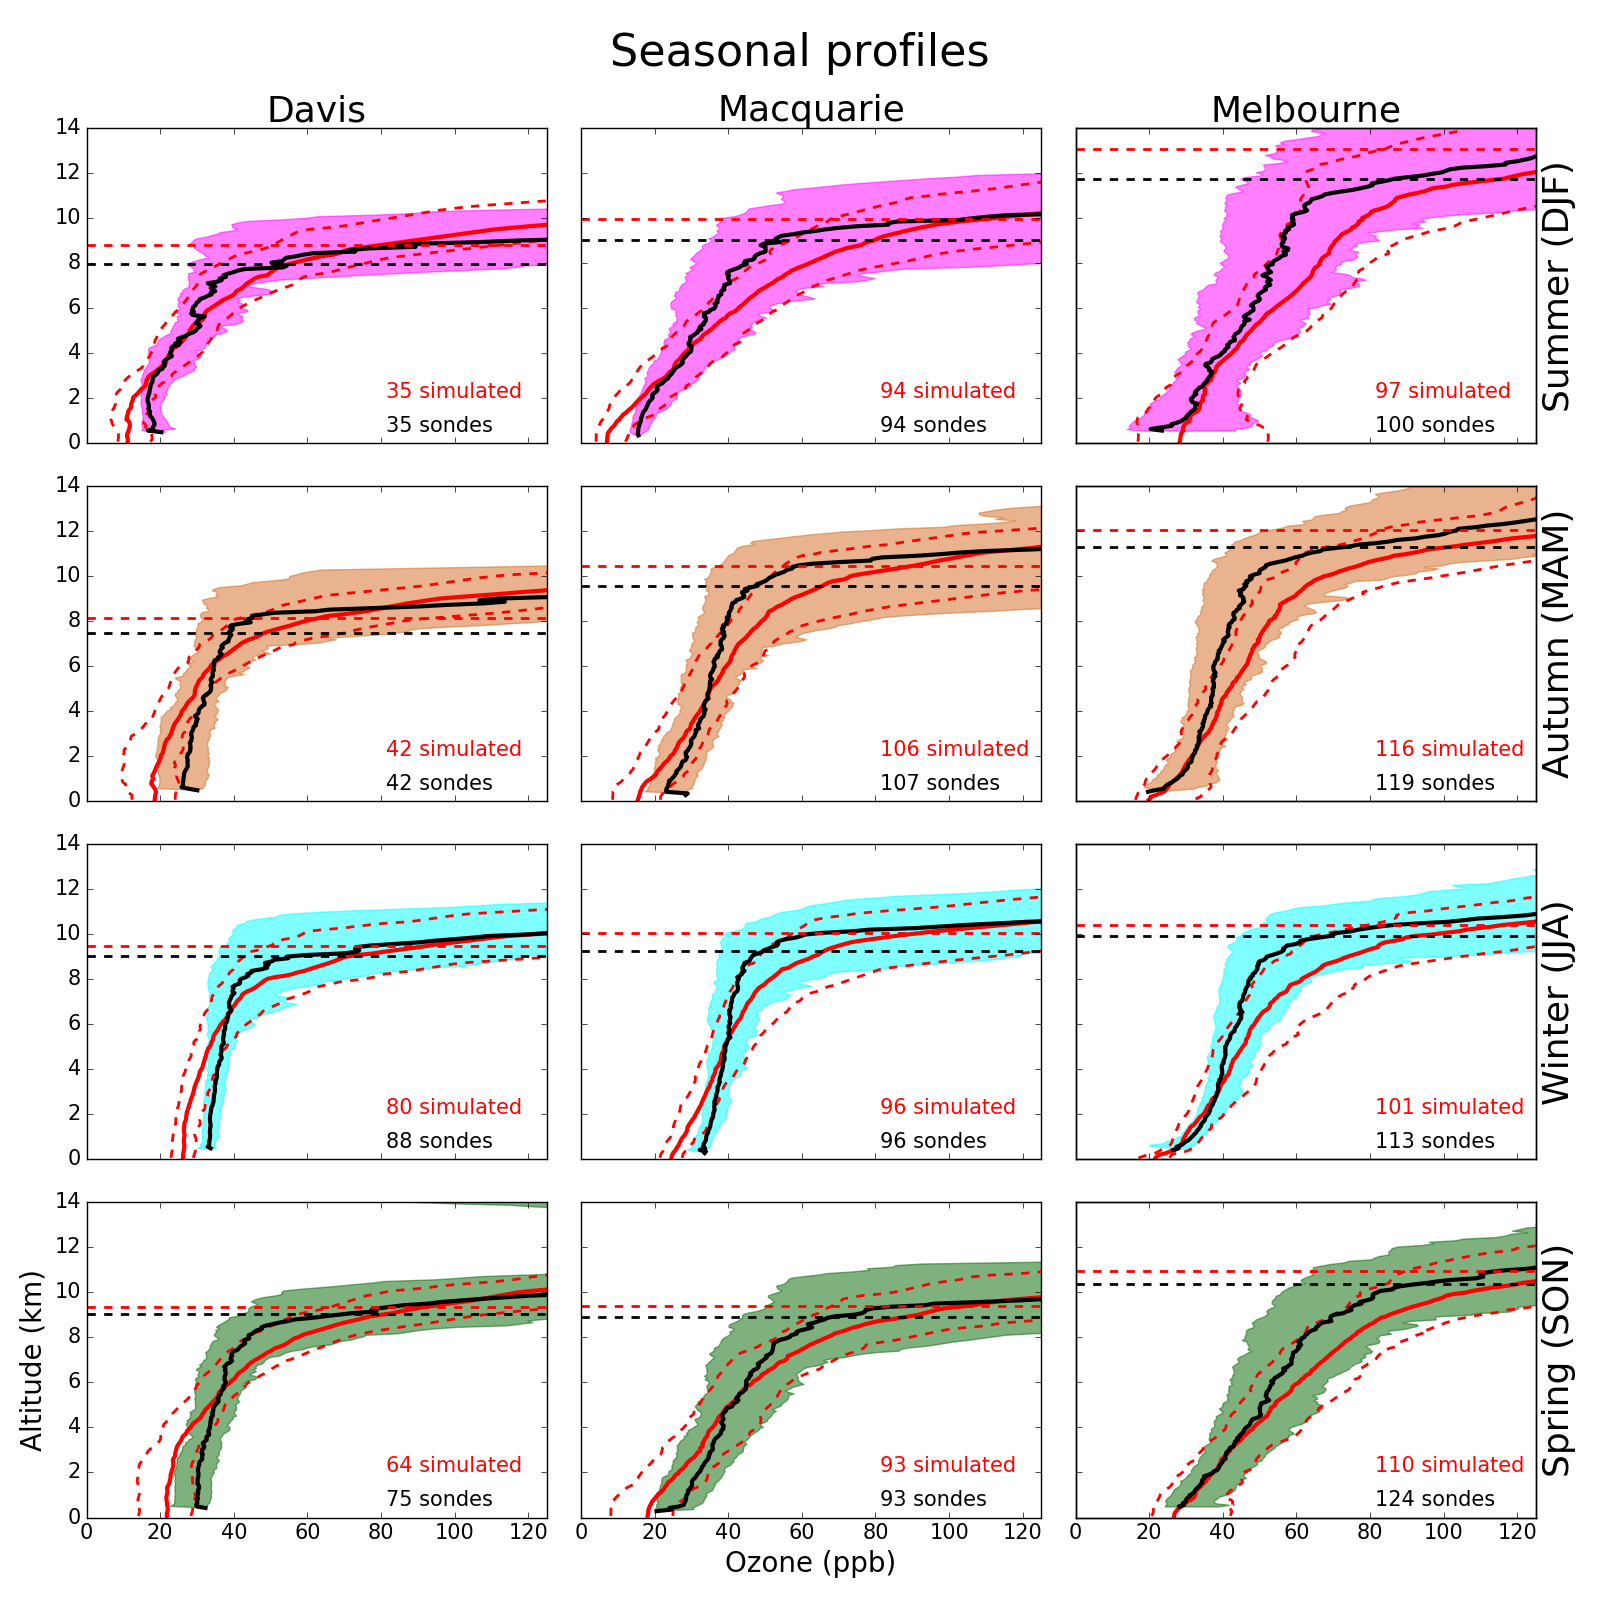
\includegraphics[width=\textwidth]{Figures/Ozone/seasonalprofiles00.png}
      \caption{Observed and simulated tropospheric ozone profiles over Davis, Macquarie, and Melbourne, averaged seasonally.
          Model means (2005-2013 average) is shown as red solid lines, with red dashed lines showing the 10th and 90th percentile.
          Ozonesonde means (over each season, for all years) are shown as black solid lines, with coloured shaded areas showing the 10th and 90th percentile.
          The horizontal dotted line shows the mean tropopause heights from the model (red) and the observations (black).}
      \label{ch_o3:fig:GEOSChemEventProfilesSummary}
    \end{figure}
    
    Considering the tropospheric ozone column, I determine the correlation between the GEOS-Chem simulated profiles and the ozone sondes using least squares linear regression.
    This assumes that the ozonesondes are the true values, while the model output is linearly dependant on them with the addition of some random error.
    This correlation is determined between simulated and measured tropospheric ozone in molecules cm$^{-2}$, for each site, for each day where there exists both a measurement and model output.
    Figure \ref{ch_o3:fig:GEOSChemTroposphereCorrelation} shows the correlation between mean modelled tropospheric ozone column.
    The colours show which season the datapoints lie within, and suggest that seasonality plays a large role in this correlation; since summer and winter points are clumped at opposite ends.
    
    \begin{figure}[!htbp]
      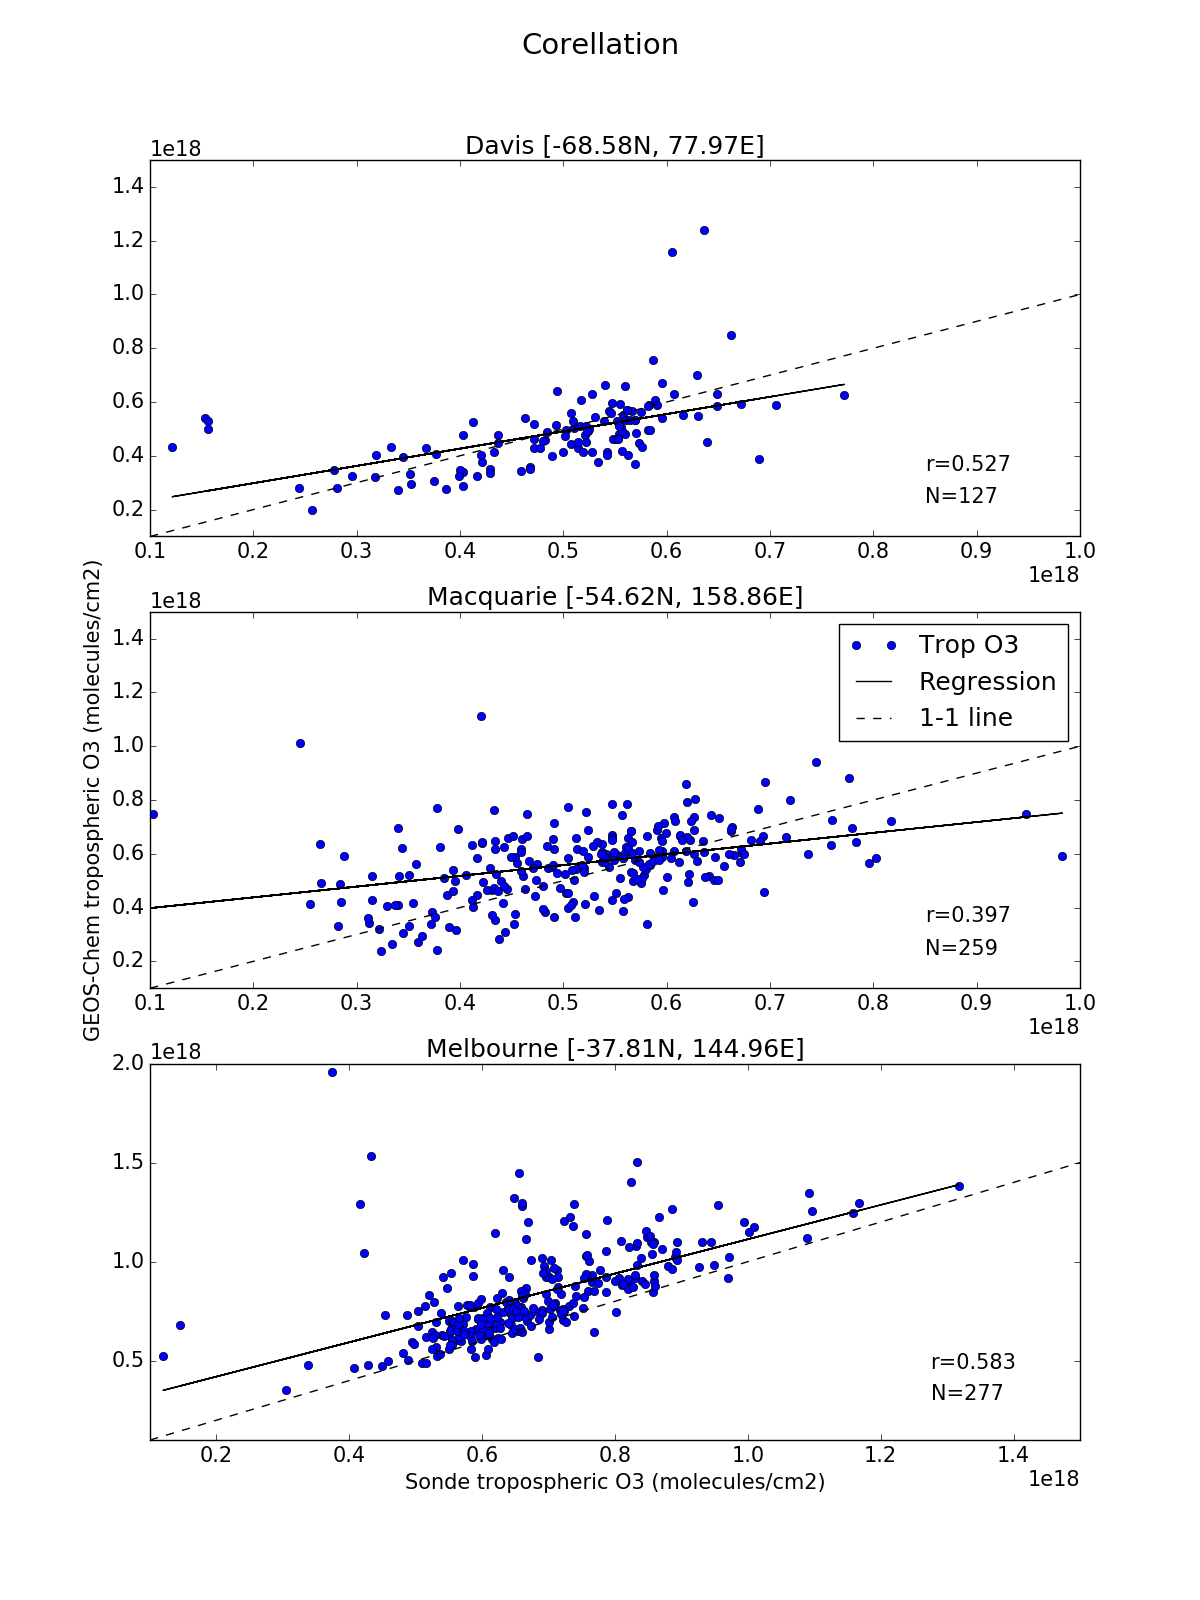
\includegraphics[width=\textwidth]{Figures/Ozone/station_correlations.png}
      \caption{Correlation between tropospheric ozone column modelled by GEOS-Chem (vertical axes) and calculated from ozone sondes (horizontal axes). 
      Points are coloured based on their season, shown by the colour bar on the right.
      The line of best fit (black) and one to one line (dashed) is also shown, note the axes are different for Melbourne.}
      \label{ch_o3:fig:GEOSChemTroposphereCorrelation}
    \end{figure}
    
    Removing the monthly mean from each dataset, and dividing by that mean gives the relative monthly difference of each datapoint from the respective dataset determined annual cycle.
    Figure \ref{ch_o3:fig:GEOSChemTroposphereCorrelationAnomalies} shows the least squares correlation between ozonesonde relative monthly anomalies and their GEOS-Chem counterparts.
    Again the season is coloured, and removal of the monthly mean removes the summer and winter clumping which could be seen in figure \ref{ch_o3:fig:GEOSChemTroposphereCorrelation}.
    The correlation coefficients are lower, since the model and the measurement both show the same seasonal trends this is expected.
    What this plot shows is the correlation between simulated tropospheric columns being above (or below) average as well as the ozonesonde measured columns being above (or below) average.
    The slopes are not one to one, which suggests the variance in sondes is not well matched by variance in simulated output.
    This effect is strongest at the Davis and Macquarie Island stations, and is exacerbated when the seasonal cycle is removed.
    
    \begin{figure}[!htbp]
      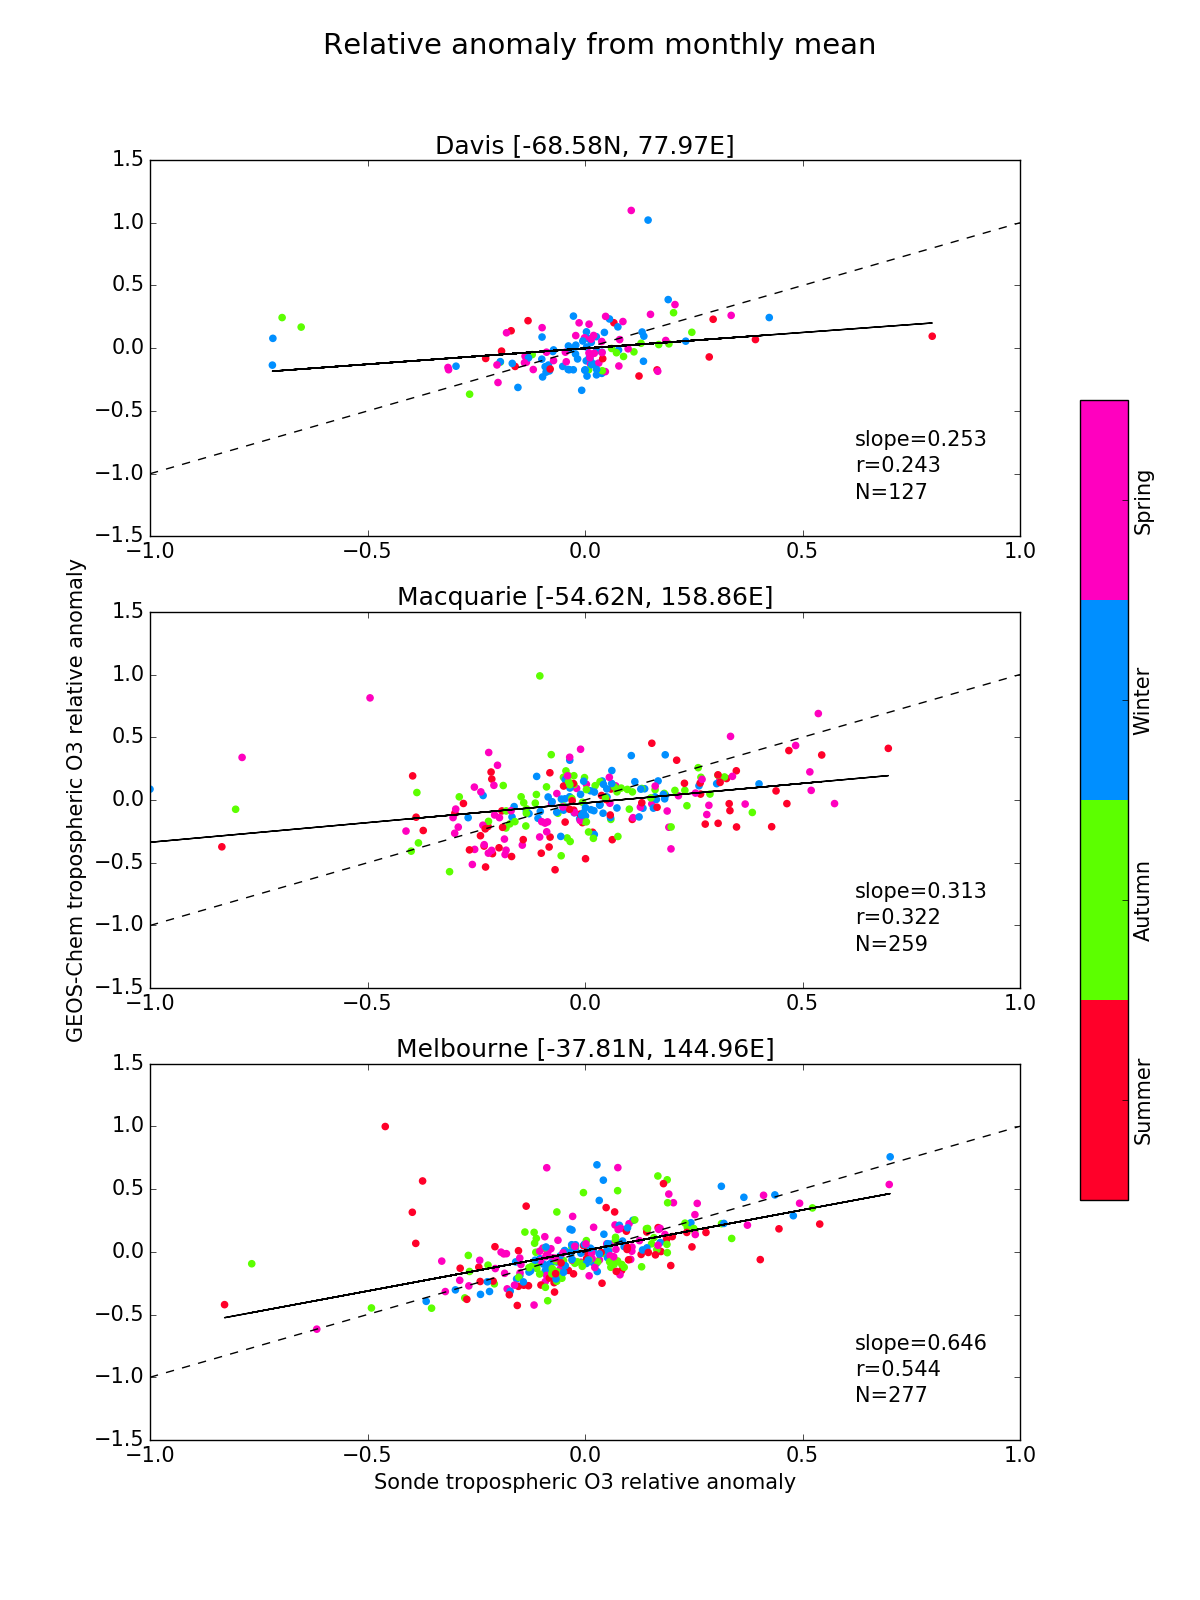
\includegraphics[width=\textwidth]{Figures/Ozone/station_correlations_anomalies.png}
      \caption{Correlation between relative difference of tropospheric ozone column from the monthly mean between profiles modelled by GEOS-Chem (vertical axes) and profiles calculated from ozone sondes (horizontal axes). 
      The line of best fit (black) and one to one line (dashed) is also shown.}
      \label{ch_o3:fig:GEOSChemTroposphereCorrelationAnomalies}
    \end{figure}
    
    (TODO: Update after model is rerun)
    Quantitatively, the modelled tropospheric profile correlates reasonably well with the ozone sonde profiles, with correlation coefficients listed in table \ref{ch_o3:tab:station_correlations}.
    Davis has a strong correlation ($r=0.527$) between sonde and simulated tropospheric column, which weakens greatly ($r=0.243$) when the season is removed.
    This suggests the model has the season and amplitude of tropospheric ozone fairly well simulated over larger time scales, but may lack accuracy when examining time periods of less than a few months.
    Macquarie and Melbourne are less affected by the removal of the seasonal cycle.
    Melbourne has a correlation coefficient greater than $0.5$ with or without the seasonal cycle, showing that the model not only represents the larger time scales fairly well, but also has some accuracy catching days which are higher or lower than the monthly average.
    
    \begin{table}
    % TODO: Update after model is rerun
    \begin{tabular}{ | c  c  c  c  c  c | }
      \hline
      \textbf{Site} & \textbf{direct} & & \textbf{anomaly$^a$} & & \textbf{compared}
      \\            & r  & r$^2$      & r & r$^2$   & \textbf{(N)}
      \\ \hline
      Davis & 0.527 & 0.278 & 0.243 & & 127
      \\
      Macquarie Island &  0.397 & 0.158 & 0.322 & & 259
      \\ %\hline
      Melbourne & 0.583 & 0.340 & 0.544 & & 277
      \\ \hline
    \end{tabular}
    \caption{Correlations between GEOS-Chem and ozonesonde tropospheric ozone column.
      \hspace{\textwidth} \\ 
      ${}^a$Relative and normalised to monthly mean from GEOS-Chem and ozone sonde for respective data. \hspace{\textwidth} \\ }
    \label{ch_o3:tab:station_correlations}
    \end{table}
        
    TODO: show modelled daily cycle?
    Recall that the profiles are output every 6 hours, so as well as getting the overall profile average it is easy to determine the daytime and night time average by only looking at particular hours.
    GEOS-Chem uses GMT/UTC time, outputting 4 profiles per day at 0~hrs, 6~hrs, 12~hrs, and 18~hrs.
    The local offset in time at Davis, Macquarie Island, and Melbourne is \+7~hrs, \+11~hrs, \+10~hrs respectively.
    
  \subsection{Estimation of southern ocean STT flux}
    A simplistic calculation of how much ozone in the southern high latitudes is due to STT is made through the following method.
    STT event likelihood, multiplied by STT event tropospheric column contribution, multiplied by southern high latitude tropospheric ozone columns, averaged seasonally.
    The monthly likelihood of STT events is determined from the ratio of detected STT events over sonde launches.
    The monthly fraction of tropospheric ozone column due to STT is calculated from the averaging the STT contributions binned by month.
    The southern high latitude tropospheric column is computed from the monthly averaged tropospheric ozone columns output by GEOS-Chem, binned into months between 2005 and 2013 inclusive.
    This modelled ozone column is the average between 55$^{\circ}$S and 85$^{\circ}$S for all longitudes.
    The equation is straightforward once the required components are all computed:
    \begin{equation*}
      Flux_i = l_i \times f_i \times tropO3_i
    \end{equation*}
    where i subscripts index the month (Jan - Dec), Flux is our estimate of STT contribution to the tropospheric ozone column, l and f represent the likelihood and contributary fraction of STT events respectively.
    Figure \ref{ch_o3:fig:SOExtrapolation} shows the seasonal STT contribution calculated this way.
    
    \begin{figure}[!htbp]
      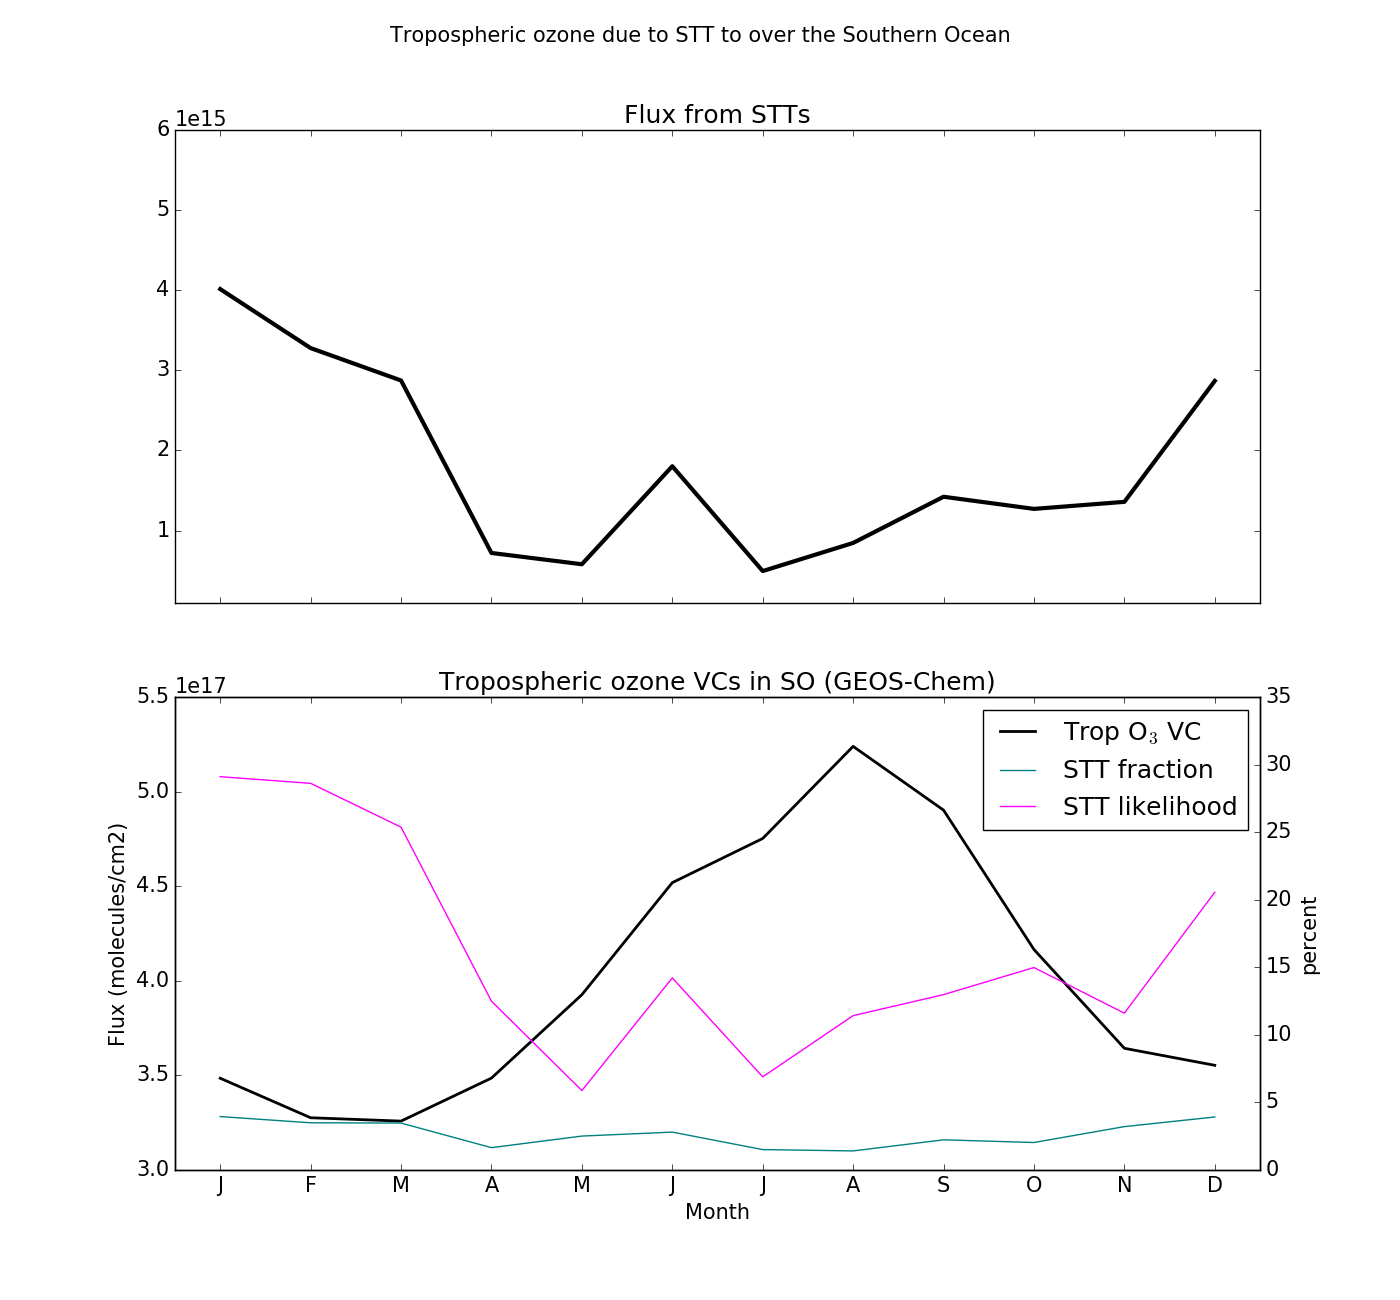
\includegraphics[width=\textwidth]{Figures/Ozone/SO_extrapolation.png}
      \caption{Top panel shows the estimated STT contribution to tropospheric ozone VC. Bottom panel shows the three factors multiplied together in order to produce the estimation. Units for l and f are on the right, while units for ozone VC amounts are on the left.}
      \label{ch_o3:fig:SOExtrapolation}
    \end{figure}
    
     % STT Ozone
% CHAPTER 3 (probably)
% Isoprene Emissions

\chapter{Isoprene Emissions in Australia} % Main chapter title
\label{ch_isop}

\section{GEOS-Chem isoprene mechanisms}
\label{ch_isop:sec:GEOSChemMechanisms}
  \subsection{Outline}
    The isoprene reactions simulated by GEOS-Chem were originally based on \cite{Horowitz1998}.
    This involved simulating NO$_X$, O$_3$, and NMHC chemistry in the troposphere at continental scale in three dimensions, with detailed NMHC chemistry with isoprene reactions and products.
    The mechanism was subsequently updated by \citet{Mao2013}, who change the isoprene nitrates yields and add products based on current understanding as laid out in \citet{Paulot2009a,Paulot2009b}.
    Further mechanistic properties, like isomerisation rates, are based citet{Crounse2011,Crounse2012,Peeters2010,Peeters2011}.
    (TODO: check abstracts of these papers)
    \cite{Crounse2011} examines the isomerisations associated with the oxidation of isoprene to six different isomers (ISO$_2$) formed in the presence of oxygen: isoprene $ + OH \rightarrow^{O_2} $ ISO$_2$.
    They determine rates and uncertainties involved in these reactions.
    \cite{Crounse2012} examine the fate of methacrolein (MACR), one of the products of isoprene oxidation. 
    Prior to this work MACR oxidation chamber studies were performed in high NO or HO$_2$ concentrations, giving peroxy lifetimes of less than 0.1~s.
    In most environments this is not the case, and MACR products over various NO concentrations and peroxy radical lifetimes are determined in their work.
    
    Formation of isoprene nitrates have an effect on ozone levels through NO$_X$ sequestration, and the yields and destinies of these nitrates is analysed in \citet{Paulot2009a}. 
    They use anion chemical ionization mass spectrometry (CIMS) to determine products of isoprene photooxidation.
    In a chamber with clean air and high NO concentrations, isoprene photooxidation is initially driven by OH addition, followed by NO$_X$ chemistry (150~min - 600~min), and finally HO$_X$ dominated chemistry.
    The yields of various positional isomers of isoprene nitrates is estimated, and pathways of their oxidation products is shown and used in the GEOS-Chem isoprene mechanism \citep{Paulot2009a,Mao2013}. 
    
    In low NO$_X$ conditions, isoprene oxidises to yield 70\% hydroxyhydroperoxides (ISOPOOH), which then oxidises to create dihydroxyperoxides (IEPOX) with OH recycling maintaining the OH levels in the atmosphere \citep{Paulot2009b}.
    In older models isoprene produced ISOPOOH which then titrated OH, however, the loss of OH has not been seen in measurements \citep{Paulot2009b,Mao2013}.
    The isoprene mechanism in GEOS-Chem has been updated to include OH regeneration from oxidation of epoxydiols and slow isomerisation of ISOPO$_2$ \citep{Mao2013}.
    
    Under high NO$_X$ conditions, isoprene undergoes OH addition at the 1 and 4 positions, becoming $\beta$ (71\%) or $\delta$ (29\%) hydroxyl peroxy radicals (ISOPO$_2$). 
    The $\beta$-hydroxyl reacts with NO$_X$ and produces HCHO (66\%), methylvinylketone (40\%) (MVK), methacrolein (26\%), and $\beta$-hydroxyl nitrates (6.7\%) (ISOPNB).
    The $\delta$-hydroxyl reacts with NO to form $\delta$-hydroxyl nitrates (24\%) (ISOPND), and ISOPNB (6.7\%).
    ISOPNB and ISOPND yield first generation isoprene at 4.7\% and 7\% respectively.
    
    Under low NO$_X$ conditions, ISOPO$_2$ may react with HO$_2$ to form ISOPOOH.
    In this case there is also production of HCHO (4.7\%), MVK(7.3\%), and MACR (12\%).
    As stated in earlier; most ISOPOOH will form IEPOX (epoxydiols) after reacting with OH and lead to OH regeneration.
    The other mechanism in low NO$_X$ environments is unimolecular isomerisation of ISOPO$_2$.
    This leads to production of hydroperoxyaldehydes (HPALDS), which generally photolyse and have an OH yield of 100\%.
    \citet{Mao2013} show that a lower (factor of 50) rate constant for ISOPO$_2$ isomerisation leads to better organic nitrate aggreements with ICARTT. 
    
    This update leads to more accurate modelling of OH concentrations, especially in low NO$_X$ conditions common in remote forests.
    Prior to \citet{Mao2012}, measurements of OH in high VOC regions may have been up to double the real atmospheric OH levels, due to formation of OH inside the instrument.
    \citet{Mao2012} examine an upgraded method of measurement, and compare these against a regional atmospheric chemistry model (RACM2), with the OH recycling updates from \citet{Paulot2009b} as discussed in prior paragraphs.
    
    The updates to isoprene chemistry by \citet{Mao2013}, and those shown in \cite{Crounse2011,Crounse2012} are the last before version 11, which was not used in this work.

    The full current mechanism is described online at \url{http://wiki.seas.harvard.edu/geos-chem/index.php/New_isoprene_scheme}.
    
  \subsection{Emissions from MEGAN}
    MEGAN simulates biogenic emissions of various gases including isoprene, based on various meteorological, land cover, and plant type parameterisations.
    
    One of the important parameters in Australia is the soil moisture activity factor($\gamma_{SM}$), which can have large regional affects on the isoprene emissions \citep{Sindelarova2014,Bauwens2016}.
    Generally if soil moisture is too low, isoprene emissions stop \citep{Pegoraro2004,Niinemets2010}, however in many Australian regions the plants may be more adapted to lower moisture levels. (TODO: Find cites for this - talk from K Emerson at Stanley indicated this)
    GEOS-Chem runs MEGANv2.1, which has three possible states for isoprene emissions based on the soil moisture ($\theta$):
    \begin{align*}
      \gamma_\mathrm{SM} & = 1 && \theta > \theta_1 \\
      \gamma_\mathrm{SM} & = (\theta-\theta_w)/\Delta\theta_1  && \theta_w < \theta < \theta_1 \\
      \gamma_\mathrm{SM} & = 0 && \theta < \theta_w \\
    \end{align*}
    where $\theta_w$ is the wilting point, and $\theta_1$ determines when plants are near the wilting point.
    The wilting point is set by a land based database from \citet{Chen2001}, while $\theta_1$ is set globally based on \citet{Pegoraro2004}. (TODO: Check Chen2001 from Guenther2006)
    
    In GEOS-Chem the emissionscan be globally multiplied by a constant factor, which was performed to determine the smearing and sensitivity.
    By running the model two extra times, with the biogenic emissions set to zero and one half, while other parameters remain unchanged, the general affects of isoprene emissions which the model undergoes can be determined.
    
%----------------------------------------------------------------------------------------
%	SECTION
%----------------------------------------------------------------------------------------
\section{Isoprene emissions estimation}
\label{ch_isop:sec:IsopreneEmissions}

  \subsection{Outline}
   With the vertical columns of biogenic HCHO we can infer the local (grid space) isoprene emissions using effective molar formaldehyde yield (In other continents around 2-3, or 1 in low NO$_X$ conditions) \citep{Palmer2003,Marais2012,Bauwens2016}.
    If we assume there is fast HCHO yield, so that the effect of chemical transport is minimal, and that HCHO and isoprene are at steady states, then we can calculate local yield from our CTM.
    %This yield is derived from both HCHO and isoprene, such as was used by \citet{Millet2006} who produced a molar HCHO yield of 2.3 in north eastern USA.
   Yield is calculated from the modelled slope between isoprene emissions and HCHO total column within each gridbox over Australia, as performed in \cite{Palmer2003}, using modelled values between 1300-1400 LT which is around the overpass time of the OMI.
   This modelled yield is then used in conjunction with the recalculated OMI measurements in order to estimate isoprene emissions.
    
    The calculations used to determine isoprene emissions over Australia are fully described in \ref{ch_isop:sec:EmissionCalculation} and follow the method of \citet{Palmer2003}.
    To calculate emissions we use a reduced major axis (RMA) regression between modelled average (from 1300-1400 LT) values of the loss rates and total columns, an example is shown in figure TODO: figure with RMA of these over whatever time and space I end up using.
    
    The measured background HCHO is the average concentration measured in the remote pacific at the same time.
    The modelled background is determined from a run with isoprene emissions turned off, which allows us to see exactly how much the modelled isoprene emissions alter each vertical column of HCHO.
    
    Isoprene quickly forms HCHO in the atmosphere when in the presence of high levels of NO$_X$.
    However, over Australia NO$_X$ levels are generally not high enough and we must take extra care that we can account for the transport or 'smearing' caused by slower HCHO formation.
    Smearing sensitive grid boxes within the model can be detected by running the model with two uniformly differing isoprene emission levels, then finding the grid boxes where the changed HCHO column is greater than can be attributed to local emission difference.
    Using equation \ref{ch_isop:eqn:isop_yield} with two different isoprene emission levels:
    \begin{equation*}
      \hat{S} = \frac{\Delta~\Omega_{HCHO}}{\Delta~E_{ISOP}}
    \end{equation*}
    Consider halving the isoprene emitted globally and rerunning the model, if the local grid HCHO is reduced by much more than half (factoring yield) then you can infer sensitivity to non-local isoprene emissions.
    This can be dependent on local or regional weather patterns, as greater wind speeds will reduce the time any emitted compound stays within the local grid box.
    As such smearing sensitivity is both spatially and temporally diverse, shown in figure TODO: is a picture of the smearing sensitivity over Australia.
   
    Once the smearing sensitive grid squares are filtered out, application of equation \ref{ch_isop:eqn:isop_yield} gives us an estimate of isoprene emissions across the nation.
    
    Most recently a \citet{Bauwens2016} undertook a similar process to what I am doing, although with slightly different focus, using the IMAGESv2 global CTM instead of GEOS-Chem.
    They calculate emissions which create the closest match between model and satellite vertical columns, and compare these postiori data with the apriori (satellite data) and independent data sets.
    (TODO: simple outline of what they did and how my focus is different, this paper will also need to be summarised in the LitReview)

  \subsection{HCHO Products and yield}
    Australian forests are strong emitters of both isoprene and monoterpenes, which go on to form various products including but not limited to secondary organic aerosols, oxygenated VOCs (OVOCs), ozone, OH, and HO$_2$.
    This production occurs over several steps, yields are often classed into at least two categories.
    First generation yield refers to the amount of HCHO produced per unit isoprene consumed by initial oxidation, total yield (sometimes molar yield) refers to time dependent yield of HCHO over multiple oxidation stages \citep{Wolfe2016}.
    \citet{Wolfe2016} define prompt yield as the change in formaldehyde measurement per unit change in initial isoprene emissions.
    Some argue that isoprene emissions are overestimated, due to the fact that they are based on relatively few measurements of isoprene emission factors \citep{Winters2009, FortemsCheiney2012} TODO: read and cite paper mentioned in Fortems.
    
    Isoprene production of HCHO depends on several factors, importantly NO$_X$ levels have a direct effect on the fate of VOCs in the atmosphere.
    At higher NO mixing ratios (at least a few hundred pptv), organic peroxy radicals (RO$_2$) react mostly with NO. 
    At low NO (less than 10's of pptv), reaction with HO$_2$, other RO$_2$, and isomerization dominate the fate of RO$_2$.
    In low NO$_X$ environments, reported HCHO yields from isoprene are from XtoY\%, while in high NO$_X$ environments this value is XtoY\% TODO: these values from table.
    For monoterpenes the yields are around X, Y\% for low, high NO$_X$ respectively.
    Emissions and yields for various species including some terpenes can be seen in table \ref{ch_isop:tab:VOCAusYields}.
    \citet{Wolfe2016} determine that going from NO$_X = 0.1$ to $2.0$ ppbv triples the prompt yield of HCHO, from 0.3 to 0.9 ppbv ppbv$^{-1}$ due to isoprene, while the background HCHO doubles.
    They determine prompt yield as the change in HCHO per change in ISOP$_0$, using $[ISOP]_0=[ISOP]\exp(k_1[\mathrm{OH}]t)$; where $k_1$ is first order loss rate.
    This effectively relates HCHO abundance with isoprene emission strength.
    (TODO:and finish Wolfe2016 discussion paper for yields)
    TODO:go through atkinsonarey2003
    
    Many of the HCHO yields from terpenoids are estimated through chamber studies which examine the products molecular mass and charge after mixing the compound of choice into a known volume of air.
    These conditions generally don't match those of the real world, where ambient air will have a cocktail of these compounds as well as various reactants.
    
    A proton transfer reaction mass spectrometer (PTR-MS) can be used to determine gas phase evolution of terpene oxidation products.
    This is done through analysis of mass to charge ratios ($m/z$) which can be used identify chemical compounds.
    Looking at Australian emissions from running GEOS-Chem and using yields provided by XYZ (TODO other table), we see that Australia may be more or less likely to do something TODO: this comparison sentence would be good to tie up tables and be copied to conclusions.
    
    Conversions between HCHO per unit C yield and molar \% yield from species X given by the equation $ Y_{molar \%} = 100 \times C_X \times Y_{HCHO per unit C} $, where $C_X$ is how many Carbon are within species X (5 for isoprene, 10 for monoterpenes, etc...).
    For instance a 200\% molar yield of HCHO from isoprene implies 1 Mole of C$_5$H$_8$ becomes 2 Mole HCHO which is a 0.4 HCHO per unit C yield.
    
    TODO: Fill out this table
    \begin{table} \begin{threeparttable}
      \caption{HCHO yields from various species averaged over Australia during Summer.}
      \begin{tabular}{ | c  c  c  c  c | }
        \toprule
	  \textbf{Species}   & \textbf{Emissions$^a$}& \textbf{Lifetime$^b$}& \textbf{HCHO Yield$^c$} & \textbf{HCHO production$^d$\%}
	  \\                 & (Tg C per month)      &                      & (per C reacted)         &         \\
	\midrule
	  Isoprene           & Y                     & n minutes            & 0.x                     & 10       \\
	  $\alpha$-Pinene    & Y                     & n minutes            & 0.x                     & 10       \\
	  $\beta$-Pinene     & Y                     & n minutes            & 0.x                     & 10       \\
	  HCHO               & Y                     & n minutes            & 1.0                     & 10       \\
	\bottomrule
      \end{tabular}
      \begin{tablenotes} 
	  \item a: Calculated using GEOS-Chem emissions over Australia in January 2005.
	  \item b:  
	  \item c: 
	  \item d: Production determined by dividing emission*yield by the sum of all VOC emissions*yields. 
      \end{tablenotes}
      \label{ch_isop:tab:VOCAusYields}
    \end{threeparttable} \end{table}
    
    % yields from Atkinsen2003
    %isoprene
    %0.63 0.10 Tuazon and Atkinson (1990a)
    %0.57 0.06 Miyoshi et al. (1994)
    % a-pinene
    %0.23 0.09 Noziere et al. (1999a)
    %0.19 0.05 Orlando et al. (2000)
    % b-pinene
    %0.54 0.05 Hatakeyama et al. (1991)
    %0.45 0.08 Orlando et al. (2000)
    
    Yields table looking at literature provided yields of HCHO.
    % molar HCHO yield per unit carbon equal to HCHO molar percent yield(per carbon)? or some conversion?
    % TODO: ask steve about ppbv ppbv^-1 ??
    
    \begin{table} \begin{threeparttable}
      \caption{ HCHO yields from various species, and lifetime against oxidation by OH. }
      \begin{tabular}{  l  l  l  l  l  }
      	\toprule
      	Species    & HCHO Yield      & Life vs OH & NO$_X$ background & Source	\\
                      & (molar \% )        &               &                          &          \\
      	\midrule 
      	Isoprene	& 315$\pm$50      &              & High           & a        \\ 
      			& 285$\pm$30      &        & High               & a        \\ 
      			& 225             & 35 min & High               & b        \\ % Done
      			& 150             &            & Low                & b        \\ % Done
      			& 150             &            & Low                & d        \\
      			& 450             &            & High               & d        \\
			& 235             &            & 1~ppbv              & e        \\
			& 150             &            & 0.1~ppbv              & e        \\
	$\alpha$-Pinene & 28$\pm$3        &        & Low                & c        \\ 
			& X$\pm$3         &        & X                  & d        \\ 
      			& 230$\pm$90      &        & High        & a        \\ 
      			& 190$\pm$50      &        & High        & a        \\ 
      			& 19                & 1 hour &              & b        \\ % Done
                      & 210               &          & 1~ppbv              & e        \\
                      & 70                &          & 0.1~ppbv              & e        \\
	$\beta$-Pinene    & 65$\pm$6        &        & Low                & c      \\ 
      			          & X$\pm$3         &        & X                  & d      \\ 
      			          & 540$\pm$50      &        & High               & a     \\ 
      			          & 450$\pm$80      &        & High               & a      \\ 
      			          & 45              & 40 min &              & b      \\ % Done
	Methane 	      & 100             & 1 year  &             & b     \\ 
	Ethane            & 180             & 10 days &             & b     \\ 
	Propane           & 60              & 2 days  &             & b     \\ 
	Methylbutanol    & .13(per C)    & 1 hour  &             & b     \\ 
	HCHO             & 100             & 2 hour  &             & b     \\ 
	Acetone           & .67(per C)      & 10 days &             & b     \\ 
	Methanol          & 100             & 2 days  &             & b     \\ %Done
    	\bottomrule
    \end{tabular}
    \begin{tablenotes} % \item makes new lines
      \item a \citet{AtkinsonArey2003}: Table 2, Yield from Isoprene reaction with OH, two values are from two referenced papers therein.
      \item b \citet{Palmer2003}: lifetimes assume [OH] is 1e15 mol cm$^{-3}$.
      \item c \citep{Lee2006}: Calculated through change in concentration of parent and product linear least squares regression.
        Estimates assume 20$^\circ$~C conditions.
  	  \item d \citet{Wolfe2016}: ``prompt yield'': change in HCHO per change in ISOP$_0$.
  	    $[ISOP]_0=[ISOP]\exp(k_1[\mathrm{OH}]t)$; where $k_1$ is first order loss rate.
  	    Effectively relates HCHO abundance with isoprene emission strength
      \item e \citet{Dufour2009}: One-day yields from oxidation modelled by CHIMERE, using MCM reference scheme.
      \item f Calculated using PTR-MS and iWAS on SENEX campaign data.
    \end{tablenotes}
    \label{ch_isop:tab:VOCLiteratureYields}
  \end{threeparttable} \end{table}
    
  \subsection{CAABA/MECCA yield}
  \label{Ch_isop:sec:CAABAMECCA}
    CAABA/MECCA is described in \ref{ch_LitRev:sec:CAABAMECCAIntro}.
    
    Using CAABA/MECCA to examine isoprene to HCHO yield in specific scenarios allows us to determine what environment may be driving the yield calculated by GEOS-Chem.
    This software runs gas and aqueous phase, and heterogeneous chemistry, including basic HO$_X$, NO$_X$, and NMHC chemistry, with emission, deposition, and initial concentrations all set.
    By running the same simulation twice, and injecting a small amount of extra isoprene into one of the simulations, extra HCHO produced can be used to determine the yield from isoprene to HCHO.
    Isoprene life time can also be calculated using this process, as the time it takes for the extra isoprene to reach $1/e$ of it's initial value.
    
    Initially we have three scenarios, grassland, desert, and forest Australia - with each scenario having initial conditions, emission and deposition set as in table \ref{ch_isop:tab:CaabaMeccaScenarioYields}.
    Running each scenario with and without a small isoprene injection gives isoprene lifetimes and isoprene to HCHO yield for those scenarios, shown in table \ref{ch_isop:tab:CaabaMeccaScenarioYields}.
    Calculation of the yield follows a calculation of the theoretical maximum carbon production by the amount of injected isoprene:
    \begin{equation}
      Y_{100} =10^9 \times \frac{C_{PM} E_{inj} D_{inj}}{(N_A H_{PBL})}
    \end{equation}
    Where Y$_{100}$ is the maximum possible carbon yield of isoprene (ppb), $C_{PM}$ is Carbon per molecule (isoprene=5), $E_{inj}$ is the emission rate of injected isoprene (molec cm$^{-2}$ s$^{-1}$), $D_{inj}$ is the duration of injection (s), H$_{PBL}$ is the boundary layer height (cm), and $N_A$ is the Air number density (molec cm$^{-3} \approx 2.5e19$).
    Finding the accumulated increase in HCHO (ppb) from the difference between the perturbed and non perturbed model runs allows calculation of the accumulated extra HCHO (Example: Figure TODO:), which divided by the $Y_{100}$ gives us the isoprene to HCHO atom C yield:
    \begin{equation}
      Y_{HCHO}= \frac{\Delta HCHO_{\text{Accumulated}}}{Y_{100}}
    \end{equation}
    with $HCHO_{\text{Accumulated}}$ being the accumulated enhanced ppb mixing ratio of HCHO.
    
    TODO: Fill in table
    \begin{table}
    	\caption{Scenario isoprene yields of HCHO}
    	\begin{tabular}{ p{6cm} l  l  l  l }
    		\hline
    		\textbf{Scenario} & \textbf{Emission} & \textbf{NO$_X$} & \textbf{HO} & Yield \\
				    		  & (molecules units) & (units)         & (units)     & units \\ \hline
    		Forest 	& xx 	& xx 	& xx 	& xx  	\\ 
    		Urban 	& xx 	& xx 	& xx 	& xx 	\\
    		Shrub 	& xx 	& xx 	& xx 	& xx 	\\ \hline
    	\end{tabular}
    	\label{ch_isop:tab:CaabaMeccaScenarioYields}
    \end{table}
    
    Figure TODO: shows the accumulated yield for all three scenarios, which each increase towards a limiting value.
    
  \subsection{Calculation of Emissions}
    \label{ch_isop:sec:EmissionCalculation}
    As is done in \citet{Palmer2003, Millet2006, Bauwens2016}, we assume that HCHO, and Isoprene columns are in a steady state, with no horizontal transport.
    In these circumstances the emissions of precursors are easy to calculate as long as we know the molar HCHO yields (Y$_i$) and effective chemical loss rates (k$_i$):
    \begin{equation}
      \Omega_{HCHO} = \frac{1}{k_{HCHO}}\Sigma_i k_i Y_i \Omega_i = \frac{1}{k_{HCHO}}\Sigma_i Y_i E_i
    \end{equation}
    
    We can infer the local (grid space) isoprene emissions (E$_{isop}$) using effective formaldehyde yield from isoprene ($Y_{isop}$).
    \begin{equation} \label{ch_isop:eqn:isop_yield}
      \Omega_{HCHO} = S \times E_{isop} + B
    \end{equation}
    Where \textit{B} is the background HCHO, and $S = Y_{isop}/k_{HCHO}$ is determined monthly as the regression between $k_{HCHO}*\Omega_{HCHO}$, and $k_{isop}*\Omega_{isop}$.
    The other equivalent method determines S from the RMA regression between $\Omega_{HCHO}$ and E$_{isop}$.
    For an initial estimate of the effective yield from simulated data: we use $k_{HCHO}$, $k_{i}$, $\Omega_{HCHO}$, and $\Omega_i$ outputs from a standard run of GEOS-Chem - which provides one data point per day.
    This gives us a value for $Y_i$ resolved to our 2$^{\circ}$ by 2.5$^{\circ}$ horizontal resolution, which is entirely based on the model, and can be compared against the yield calculated using OMI derived $\Omega_{HCHO}$.
    Using our measurements of the biogenic HCHO column ($\Omega_{OMIHCHO}$) recalculated from the OMI satellite product, we derive yield using the same method and determine our new top-down emissions estimates.
    Figure ()TODO: figure with RMA of these over whatever time and space I end up using.) shows the modelled isoprene emissions and column concentrations along with the RMA regression line - which leads to an estimated yield of TODO
    
    This works if there is fast HCHO yield, so that the effect of chemical transport is minimal.
    The background HCHO is calculated using measurements in the remote pacific at the same time and latitude.
    Table \ref{ch_isop:tab:VOCAusYields} shows the average yield calculated for Australia. (TODO: this table and some notes)
    
  \subsection{Calculation of smearing effect}
    TODO: Smearing scale length, $\hat{S}$ formula, and results of calculations in here.
    As shown in \cite{Palmer2003}, smearing sensitivity can be calculated through multiple runs of the same model with the only difference being the isoprene emissions.
    I have run GEOS-Chem with and without E$_{ISOP}$ multiplied uniformly by 0.5, and the grid boxes with the most affected $\Omega_{HCHO}$ are those affected most by smearing.
    The smearing parameter  ($\hat{S}$) is defined as follows:
    \begin{equation}
      \hat{S} = \frac{\Delta \Omega_{HCHO}}{\Delta E_{ISOP}}
    \end{equation}
    TODO: Plot shows smearing parameter over Australia.
  
  \subsection{Calculations of uncertainty}
    There are several factors which need to be considered when looking at the uncertainty in emissions estimates.
    Things with their own inherent uncertainty include the modelled apriori, modelled relationship between HCHO and isoprene, and satellite measurements. 
    Important factors which need to be analysed for confidence in results include the steady state assumptions, filtering techniques for fire and human influences, and the regression model for determining the isoprene to HCHO yield.

    Uncertainty in satellite measurements is generally provided along with the data, although uncertainty introduced through AMF calculation needs to be determined to give a representation of the confidence in vertical column amounts.
    The measurement uncertainty is shown in section \ref{ch_HCHO:sec:OMI_uncertainty_calculation}, and amounts to $\sim X%$. (TODO this number when calculated)
    
    Model uncertainty is difficult to accurately assertain, generally an analysis of the model compared to in-situ measurements is performed, however there are few of these measurements over Australia.
    TODO: find out how this is estimated in other papers, or else point to HCHO uncertainty and used some function of that.
    
    The uncertainty for HCHO to isoprene mechanisms TODO: how to do this?
  
  \subsection{Extrapolating the circadian cycle}
    Isoprene emissions occur with regular daily cycles caused by things like local temperature, sunlight, drought, and other environmental factors (TODO: find/cite eucalypt isoprene paper, daily cycle plot if can find).
    
    (TODO: following stuff, add some basic plots and error analysis eventually also)
    Using a model of the daily isoprene emissions fit to the offset determined by satellite HCHO based estimates, we produce a high temporal resolution isoprene emissions inventory.
    During days with more than one HCHO column measurement we can more confidently fit the cycle. 
    For example EOS AURA's OMI measurements from 2004 can be combined with MetOp-A's GOME2 after October 2006, with daily overpasses by OMI and GOME2 at 1345 and 0930 respectively.
    This allows a better retrieval of the daily amplitude of isoprene emissions.
    
  \subsection{Comparison with MEGAN}
    TODO: Direct comparison here, maps of differences for some metrics(monthly average,?). comparison of model run results using different inventory shown in section (reference here)

\section{New estimates affects on the Australian atmosphere}

 % Isoprene
%\input{Chapters/Chapter4} % Model Resolution
%\input{Chapters/Chapter5} % DUST?!

%----------------------------------------------------------------------------------------
%	THESIS CONTENT - APPENDICES
%----------------------------------------------------------------------------------------

\appendix % Cue to tell LaTeX that the following "chapters" are Appendices

% Include the appendices of the thesis as separate files from the Appendices folder
% Uncomment the lines as you write the Appendices

%% Appendix A

\chapter{Appendix A} % Main appendix title
\label{app_a}

% figures.tex created in python in appendices folder
%\section{Melbourne}
  \includegraphics[width=\textwidth]{../OzoneWork/Images/AIRS/Melbourne/2007-01-12.png}
  \includegraphics[width=\textwidth]{../OzoneWork/Images/AIRS/Melbourne/2011-08-24.png}
  \includegraphics[width=\textwidth]{../OzoneWork/Images/AIRS/Melbourne/2012-10-30.png}
  \includegraphics[width=\textwidth]{../OzoneWork/Images/AIRS/Melbourne/2011-03-09.png}
  \includegraphics[width=\textwidth]{../OzoneWork/Images/AIRS/Melbourne/2013-01-16.png}
  \includegraphics[width=\textwidth]{../OzoneWork/Images/AIRS/Melbourne/2007-04-20.png}
  \includegraphics[width=\textwidth]{../OzoneWork/Images/AIRS/Melbourne/2005-11-08.png}
  \includegraphics[width=\textwidth]{../OzoneWork/Images/AIRS/Melbourne/2011-05-11.png}
  \includegraphics[width=\textwidth]{../OzoneWork/Images/AIRS/Melbourne/2006-02-03.png}
  \includegraphics[width=\textwidth]{../OzoneWork/Images/AIRS/Melbourne/2008-02-21.png}
  \includegraphics[width=\textwidth]{../OzoneWork/Images/AIRS/Melbourne/2009-01-07.png}
  \includegraphics[width=\textwidth]{../OzoneWork/Images/AIRS/Melbourne/2012-02-23.png}
  \includegraphics[width=\textwidth]{../OzoneWork/Images/AIRS/Melbourne/2011-02-23.png}
  \includegraphics[width=\textwidth]{../OzoneWork/Images/AIRS/Melbourne/2013-01-04.png}
  \includegraphics[width=\textwidth]{../OzoneWork/Images/AIRS/Melbourne/2007-10-17.png}
  \includegraphics[width=\textwidth]{../OzoneWork/Images/AIRS/Melbourne/2013-01-11.png}
  \includegraphics[width=\textwidth]{../OzoneWork/Images/AIRS/Melbourne/2011-03-16.png}
  \includegraphics[width=\textwidth]{../OzoneWork/Images/AIRS/Melbourne/2006-10-16.png}
  \includegraphics[width=\textwidth]{../OzoneWork/Images/AIRS/Melbourne/2009-01-13.png}
  \includegraphics[width=\textwidth]{../OzoneWork/Images/AIRS/Melbourne/2008-11-26.png}
  \includegraphics[width=\textwidth]{../OzoneWork/Images/AIRS/Melbourne/2013-03-20.png}
  \includegraphics[width=\textwidth]{../OzoneWork/Images/AIRS/Melbourne/2007-04-13.png}
  \includegraphics[width=\textwidth]{../OzoneWork/Images/AIRS/Melbourne/2011-07-13.png}
  \includegraphics[width=\textwidth]{../OzoneWork/Images/AIRS/Melbourne/2008-12-03.png}
  \includegraphics[width=\textwidth]{../OzoneWork/Images/AIRS/Melbourne/2009-09-23.png}
  \includegraphics[width=\textwidth]{../OzoneWork/Images/AIRS/Melbourne/2010-10-27.png}
  \includegraphics[width=\textwidth]{../OzoneWork/Images/AIRS/Melbourne/2011-02-17.png}
  \includegraphics[width=\textwidth]{../OzoneWork/Images/AIRS/Melbourne/2009-09-16.png}
  \includegraphics[width=\textwidth]{../OzoneWork/Images/AIRS/Melbourne/2010-09-02.png}
  \includegraphics[width=\textwidth]{../OzoneWork/Images/AIRS/Melbourne/2012-03-14.png}
  \includegraphics[width=\textwidth]{../OzoneWork/Images/AIRS/Melbourne/2013-05-01.png}
  \includegraphics[width=\textwidth]{../OzoneWork/Images/AIRS/Melbourne/2007-01-04.png}
  \includegraphics[width=\textwidth]{../OzoneWork/Images/AIRS/Melbourne/2010-07-07.png}
  \includegraphics[width=\textwidth]{../OzoneWork/Images/AIRS/Melbourne/2006-02-17.png}
  \includegraphics[width=\textwidth]{../OzoneWork/Images/AIRS/Melbourne/2012-10-03.png}
  \includegraphics[width=\textwidth]{../OzoneWork/Images/AIRS/Melbourne/2005-01-13.png}
  \includegraphics[width=\textwidth]{../OzoneWork/Images/AIRS/Melbourne/2011-12-07.png}
  \includegraphics[width=\textwidth]{../OzoneWork/Images/AIRS/Melbourne/2008-07-09.png}
  \includegraphics[width=\textwidth]{../OzoneWork/Images/AIRS/Melbourne/2004-10-07.png}
  \includegraphics[width=\textwidth]{../OzoneWork/Images/AIRS/Melbourne/2010-03-10.png}
  \includegraphics[width=\textwidth]{../OzoneWork/Images/AIRS/Melbourne/2010-06-02.png}
  \includegraphics[width=\textwidth]{../OzoneWork/Images/AIRS/Melbourne/2006-08-09.png}
  \includegraphics[width=\textwidth]{../OzoneWork/Images/AIRS/Melbourne/2011-02-15.png}
  \includegraphics[width=\textwidth]{../OzoneWork/Images/AIRS/Melbourne/2011-10-25.png}
  \includegraphics[width=\textwidth]{../OzoneWork/Images/AIRS/Melbourne/2008-12-12.png}
  \includegraphics[width=\textwidth]{../OzoneWork/Images/AIRS/Melbourne/2010-01-28.png}
  \includegraphics[width=\textwidth]{../OzoneWork/Images/AIRS/Melbourne/2011-04-20.png}
  \includegraphics[width=\textwidth]{../OzoneWork/Images/AIRS/Melbourne/2005-10-26.png}
  \includegraphics[width=\textwidth]{../OzoneWork/Images/AIRS/Melbourne/2008-01-18.png}
  \includegraphics[width=\textwidth]{../OzoneWork/Images/AIRS/Melbourne/2009-01-30.png}
  \includegraphics[width=\textwidth]{../OzoneWork/Images/AIRS/Melbourne/2009-12-23.png}
  \includegraphics[width=\textwidth]{../OzoneWork/Images/AIRS/Melbourne/2013-02-01.png}
  \includegraphics[width=\textwidth]{../OzoneWork/Images/AIRS/Melbourne/2006-03-02.png}
  \includegraphics[width=\textwidth]{../OzoneWork/Images/AIRS/Melbourne/2010-01-13.png}
  \includegraphics[width=\textwidth]{../OzoneWork/Images/AIRS/Melbourne/2006-07-20.png}
  \includegraphics[width=\textwidth]{../OzoneWork/Images/AIRS/Melbourne/2004-01-08.png}
  \includegraphics[width=\textwidth]{../OzoneWork/Images/AIRS/Melbourne/2005-04-14.png}
  \includegraphics[width=\textwidth]{../OzoneWork/Images/AIRS/Melbourne/2005-11-03.png}
  \includegraphics[width=\textwidth]{../OzoneWork/Images/AIRS/Melbourne/2010-02-03.png}
  \includegraphics[width=\textwidth]{../OzoneWork/Images/AIRS/Melbourne/2007-03-15.png}
  \includegraphics[width=\textwidth]{../OzoneWork/Images/AIRS/Melbourne/2011-02-09.png}
  \includegraphics[width=\textwidth]{../OzoneWork/Images/AIRS/Melbourne/2009-07-21.png}
  \includegraphics[width=\textwidth]{../OzoneWork/Images/AIRS/Melbourne/2010-11-03.png}
  \includegraphics[width=\textwidth]{../OzoneWork/Images/AIRS/Melbourne/2009-09-02.png}
  \includegraphics[width=\textwidth]{../OzoneWork/Images/AIRS/Melbourne/2010-04-07.png}
  \includegraphics[width=\textwidth]{../OzoneWork/Images/AIRS/Melbourne/2005-11-17.png}
  \includegraphics[width=\textwidth]{../OzoneWork/Images/AIRS/Melbourne/2010-03-04.png}
  \includegraphics[width=\textwidth]{../OzoneWork/Images/AIRS/Melbourne/2012-12-21.png}
  \includegraphics[width=\textwidth]{../OzoneWork/Images/AIRS/Melbourne/2004-02-02.png}
  \includegraphics[width=\textwidth]{../OzoneWork/Images/AIRS/Melbourne/2007-03-28.png}
  \includegraphics[width=\textwidth]{../OzoneWork/Images/AIRS/Melbourne/2013-10-04.png}
  \includegraphics[width=\textwidth]{../OzoneWork/Images/AIRS/Melbourne/2007-10-31.png}
  \includegraphics[width=\textwidth]{../OzoneWork/Images/AIRS/Melbourne/2007-03-21.png}
\section{Macquarie}
  \includegraphics[width=\textwidth]{../OzoneWork/Images/AIRS/Macquarie/2009-02-18.png}
  \includegraphics[width=\textwidth]{../OzoneWork/Images/AIRS/Macquarie/2004-02-04.png}
  \includegraphics[width=\textwidth]{../OzoneWork/Images/AIRS/Macquarie/2011-05-11.png}
  \includegraphics[width=\textwidth]{../OzoneWork/Images/AIRS/Macquarie/2004-05-19.png}
  \includegraphics[width=\textwidth]{../OzoneWork/Images/AIRS/Macquarie/2005-08-25.png}
  \includegraphics[width=\textwidth]{../OzoneWork/Images/AIRS/Macquarie/2010-02-10.png}
  \includegraphics[width=\textwidth]{../OzoneWork/Images/AIRS/Macquarie/2009-01-21.png}
  \includegraphics[width=\textwidth]{../OzoneWork/Images/AIRS/Macquarie/2005-01-12.png}
  \includegraphics[width=\textwidth]{../OzoneWork/Images/AIRS/Macquarie/2009-01-07.png}
  \includegraphics[width=\textwidth]{../OzoneWork/Images/AIRS/Macquarie/2010-02-24.png}
  \includegraphics[width=\textwidth]{../OzoneWork/Images/AIRS/Macquarie/2010-01-27.png}
  \includegraphics[width=\textwidth]{../OzoneWork/Images/AIRS/Macquarie/2008-03-21.png}
  \includegraphics[width=\textwidth]{../OzoneWork/Images/AIRS/Macquarie/2005-01-19.png}
  \includegraphics[width=\textwidth]{../OzoneWork/Images/AIRS/Macquarie/2006-10-12.png}
  \includegraphics[width=\textwidth]{../OzoneWork/Images/AIRS/Macquarie/2012-12-19.png}
  \includegraphics[width=\textwidth]{../OzoneWork/Images/AIRS/Macquarie/2007-01-17.png}
  \includegraphics[width=\textwidth]{../OzoneWork/Images/AIRS/Macquarie/2004-03-10.png}
  \includegraphics[width=\textwidth]{../OzoneWork/Images/AIRS/Macquarie/2008-06-04.png}
  \includegraphics[width=\textwidth]{../OzoneWork/Images/AIRS/Macquarie/2004-06-09.png}
  \includegraphics[width=\textwidth]{../OzoneWork/Images/AIRS/Macquarie/2010-03-31.png}
  \includegraphics[width=\textwidth]{../OzoneWork/Images/AIRS/Macquarie/2009-01-14.png}
  \includegraphics[width=\textwidth]{../OzoneWork/Images/AIRS/Macquarie/2008-10-22.png}
  \includegraphics[width=\textwidth]{../OzoneWork/Images/AIRS/Macquarie/2004-03-05.png}
  \includegraphics[width=\textwidth]{../OzoneWork/Images/AIRS/Macquarie/2009-12-09.png}
  \includegraphics[width=\textwidth]{../OzoneWork/Images/AIRS/Macquarie/2005-12-21.png}
  \includegraphics[width=\textwidth]{../OzoneWork/Images/AIRS/Macquarie/2011-04-06.png}
  \includegraphics[width=\textwidth]{../OzoneWork/Images/AIRS/Macquarie/2009-09-09.png}
  \includegraphics[width=\textwidth]{../OzoneWork/Images/AIRS/Macquarie/2004-10-20.png}
  \includegraphics[width=\textwidth]{../OzoneWork/Images/AIRS/Macquarie/2011-12-07.png}
  \includegraphics[width=\textwidth]{../OzoneWork/Images/AIRS/Macquarie/2009-08-26.png}
  \includegraphics[width=\textwidth]{../OzoneWork/Images/AIRS/Macquarie/2011-02-16.png}
  \includegraphics[width=\textwidth]{../OzoneWork/Images/AIRS/Macquarie/2010-03-10.png}
  \includegraphics[width=\textwidth]{../OzoneWork/Images/AIRS/Macquarie/2011-01-19.png}
  \includegraphics[width=\textwidth]{../OzoneWork/Images/AIRS/Macquarie/2011-09-21.png}
  \includegraphics[width=\textwidth]{../OzoneWork/Images/AIRS/Macquarie/2009-06-24.png}
  \includegraphics[width=\textwidth]{../OzoneWork/Images/AIRS/Macquarie/2005-03-28.png}
  \includegraphics[width=\textwidth]{../OzoneWork/Images/AIRS/Macquarie/2009-12-23.png}
  \includegraphics[width=\textwidth]{../OzoneWork/Images/AIRS/Macquarie/2012-03-29.png}
  \includegraphics[width=\textwidth]{../OzoneWork/Images/AIRS/Macquarie/2005-10-19.png}
  \includegraphics[width=\textwidth]{../OzoneWork/Images/AIRS/Macquarie/2008-02-13.png}
  \includegraphics[width=\textwidth]{../OzoneWork/Images/AIRS/Macquarie/2006-02-01.png}
  \includegraphics[width=\textwidth]{../OzoneWork/Images/AIRS/Macquarie/2009-03-18.png}
  \includegraphics[width=\textwidth]{../OzoneWork/Images/AIRS/Macquarie/2012-08-09.png}
  \includegraphics[width=\textwidth]{../OzoneWork/Images/AIRS/Macquarie/2011-02-03.png}
  \includegraphics[width=\textwidth]{../OzoneWork/Images/AIRS/Macquarie/2004-02-25.png}
  \includegraphics[width=\textwidth]{../OzoneWork/Images/AIRS/Macquarie/2012-09-26.png}
  \includegraphics[width=\textwidth]{../OzoneWork/Images/AIRS/Macquarie/2006-11-08.png}
  \includegraphics[width=\textwidth]{../OzoneWork/Images/AIRS/Macquarie/2012-08-16.png}
  \includegraphics[width=\textwidth]{../OzoneWork/Images/AIRS/Macquarie/2007-03-14.png}
  \includegraphics[width=\textwidth]{../OzoneWork/Images/AIRS/Macquarie/2007-03-08.png}
\section{Davis}
  \includegraphics[width=\textwidth]{../OzoneWork/Images/AIRS/Davis/2012-11-24.png}
  \includegraphics[width=\textwidth]{../OzoneWork/Images/AIRS/Davis/2011-03-09.png}
  \includegraphics[width=\textwidth]{../OzoneWork/Images/AIRS/Davis/2011-12-14.png}
  \includegraphics[width=\textwidth]{../OzoneWork/Images/AIRS/Davis/2011-01-12.png}
  \includegraphics[width=\textwidth]{../OzoneWork/Images/AIRS/Davis/2011-04-13.png}
  \includegraphics[width=\textwidth]{../OzoneWork/Images/AIRS/Davis/2012-12-03.png}
  \includegraphics[width=\textwidth]{../OzoneWork/Images/AIRS/Davis/2011-06-29.png}
  \includegraphics[width=\textwidth]{../OzoneWork/Images/AIRS/Davis/2007-01-15.png}
  \includegraphics[width=\textwidth]{../OzoneWork/Images/AIRS/Davis/2012-03-21.png}
  \includegraphics[width=\textwidth]{../OzoneWork/Images/AIRS/Davis/2008-06-04.png}
  \includegraphics[width=\textwidth]{../OzoneWork/Images/AIRS/Davis/2012-10-13.png}
  \includegraphics[width=\textwidth]{../OzoneWork/Images/AIRS/Davis/2008-06-11.png}
  \includegraphics[width=\textwidth]{../OzoneWork/Images/AIRS/Davis/2008-10-22.png}
  \includegraphics[width=\textwidth]{../OzoneWork/Images/AIRS/Davis/2009-09-23.png}
  \includegraphics[width=\textwidth]{../OzoneWork/Images/AIRS/Davis/2010-09-23.png}
  \includegraphics[width=\textwidth]{../OzoneWork/Images/AIRS/Davis/2009-07-01.png}
  \includegraphics[width=\textwidth]{../OzoneWork/Images/AIRS/Davis/2012-07-19.png}
  \includegraphics[width=\textwidth]{../OzoneWork/Images/AIRS/Davis/2006-09-30.png}
  \includegraphics[width=\textwidth]{../OzoneWork/Images/AIRS/Davis/2010-12-10.png}
  \includegraphics[width=\textwidth]{../OzoneWork/Images/AIRS/Davis/2011-03-04.png}
  \includegraphics[width=\textwidth]{../OzoneWork/Images/AIRS/Davis/2006-09-22.png}
  \includegraphics[width=\textwidth]{../OzoneWork/Images/AIRS/Davis/2012-02-15.png}
  \includegraphics[width=\textwidth]{../OzoneWork/Images/AIRS/Davis/2013-10-23.png}
  \includegraphics[width=\textwidth]{../OzoneWork/Images/AIRS/Davis/2012-04-12.png}
  \includegraphics[width=\textwidth]{../OzoneWork/Images/AIRS/Davis/2009-06-24.png}
  \includegraphics[width=\textwidth]{../OzoneWork/Images/AIRS/Davis/2007-08-11.png}
  \includegraphics[width=\textwidth]{../OzoneWork/Images/AIRS/Davis/2007-12-11.png}
  \includegraphics[width=\textwidth]{../OzoneWork/Images/AIRS/Davis/2009-11-21.png}
  \includegraphics[width=\textwidth]{../OzoneWork/Images/AIRS/Davis/2007-04-17.png}
  \includegraphics[width=\textwidth]{../OzoneWork/Images/AIRS/Davis/2008-03-14.png}
  \includegraphics[width=\textwidth]{../OzoneWork/Images/AIRS/Davis/2006-06-06.png}
  \includegraphics[width=\textwidth]{../OzoneWork/Images/AIRS/Davis/2011-07-20.png}
  \includegraphics[width=\textwidth]{../OzoneWork/Images/AIRS/Davis/2009-10-07.png}
  \includegraphics[width=\textwidth]{../OzoneWork/Images/AIRS/Davis/2012-01-25.png}
  \includegraphics[width=\textwidth]{../OzoneWork/Images/AIRS/Davis/2007-02-16.png}
  \includegraphics[width=\textwidth]{../OzoneWork/Images/AIRS/Davis/2013-08-21.png}

  
\section{Grid Resolution}
% grid created using ctm_grid output -> text created by levels_table.py in extras
\begin{table}
  \begin{tabular}{|l|c|c|}
    \hline
    Level & z(km) & eta 
    \\ \hline
    1 & 0.058483 & 0.99250000 
    \\ \hline
    2 & 0.188515 & 0.97745600 
    \\ \hline
    3 & 0.320427 & 0.96237000 
    \\ \hline
    4 & 0.453892 & 0.94728500 
    \\ \hline
    5 & 0.588963 & 0.93220000 
    \\ \hline
    6 & 0.725697 & 0.91711600 
    \\ \hline
    7 & 0.864132 & 0.90203100 
    \\ \hline
    8 & 1.004320 & 0.88694800 
    \\ \hline
    9 & 1.146330 & 0.87186400 
    \\ \hline
    10 & 1.290220 & 0.85678100 
    \\ \hline
    11 & 1.436040 & 0.84169800 
    \\ \hline
    12 & 1.583870 & 0.82661600 
    \\ \hline
    13 & 1.758950 & 0.80902100 
    \\ \hline
    14 & 1.988400 & 0.78640000 
    \\ \hline
    15 & 2.249380 & 0.76126500 
    \\ \hline
    16 & 2.517070 & 0.73613400 
    \\ \hline
    17 & 2.791920 & 0.71100600 
    \\ \hline
    18 & 3.074460 & 0.68587800 
    \\ \hline
    19 & 3.439220 & 0.65447100 
    \\ \hline
    20 & 3.895550 & 0.61679000 
    \\ \hline
    21 & 4.374520 & 0.57911500 
    \\ \hline
    22 & 4.879030 & 0.54144900 
    \\ \hline
    23 & 5.412570 & 0.50379500 
    \\ \hline
    24 & 5.979530 & 0.46615300 
    \\ \hline
    25 & 6.585330 & 0.42852800 
    \\ \hline
    26 & 7.236820 & 0.39092700 
    \\ \hline
    27 & 7.943070 & 0.35334900 
    \\ \hline
    28 & 8.845840 & 0.30985400 
    \\ \hline
    29 & 9.936460 & 0.26358700 
    \\ \hline
    30 & 11.020800 & 0.22377200 
    \\ \hline
    31 & 12.085500 & 0.19006100 
    \\ \hline
    32 & 13.133500 & 0.16151300 
    \\ \hline
    33 & 14.169600 & 0.13728700 
    \\ \hline
    34 & 15.198200 & 0.11669500 
    \\ \hline
    35 & 16.221700 & 0.09919110 
    \\ \hline
    36 & 17.242600 & 0.08431270 
    \\ \hline
    37 & 18.727200 & 0.06655890 
    \\ \hline
    38 & 20.835700 & 0.04764090 
    \\ \hline
    39 & 23.020500 & 0.03381390 
    \\ \hline
    40 & 25.306800 & 0.02375520 
    \\ \hline
    41 & 28.654300 & 0.01434240 
    \\ \hline
    42 & 34.024400 & 0.00658754 
    \\ \hline
    43 & 40.166100 & 0.00281639 
    \\ \hline
    44 & 47.135400 & 0.00110910 
    \\ \hline
    45 & 54.833600 & 0.00039878 
    \\ \hline
    46 & 63.052800 & 0.00012699 
    \\ \hline
    47 & 72.180100 & 0.00002763 
    \\ \hline
  \end{tabular}
  \caption{The 47 level vertical grid used by GEOS-Chem}
  \label{app_a:tab:gc_47_vgrid}
\end{table} % this one has all the AIRS images (3/page)



%\input{Appendices/AppendixC}

%----------------------------------------------------------------------------------------
%	BIBLIOGRAPHY
%----------------------------------------------------------------------------------------

\printbibliography[heading=bibintoc]

%----------------------------------------------------------------------------------------

\end{document}  
